\documentclass[10pt]{book}
\usepackage[text=17cm,left=2.5cm,right=2.5cm, headsep=20pt, top=2.5cm, bottom = 2cm,letterpaper,showframe = false]{geometry} %configuración página
\usepackage{latexsym,amsmath,amssymb,amsfonts} %(símbolos de la AMS).7
\parindent = 0cm  %sangria
\usepackage[T1]{fontenc} %acentos en español
\usepackage[spanish]{babel} %español capitulos y secciones
\usepackage{graphicx} %gráficos y figuras.

%---------------FORMATO de letra--------------------%

\usepackage{lmodern} % tipos de letras
\usepackage{titlesec} %formato de títulos
\usepackage[backref=page]{hyperref} %hipervinculos
\usepackage{multicol} %columnas
\usepackage{tcolorbox, empheq} %cajas
\usepackage{enumerate} %indice enumerado
\usepackage{marginnote}%notas en el margen
\tcbuselibrary{skins,breakable,listings,theorems}
\usepackage[Bjornstrup]{fncychap}%diseño de portada de capitulos
\usepackage[all]{xy}%flechas
\counterwithout{footnote}{chapter}
\usepackage{xcolor}
\usepackage[htt]{hyphenat}
%--------------------GRÀFICOS--------------------------

\usepackage{tkz-fct}

%---------------------------------

\titleformat*{\section}{\bfseries\rmfamily}
\titleformat*{\subsection}{\bfseries\rmfamily}
\titleformat*{\subsubsection}{\bfseries\rmfamily}
\titleformat*{\paragraph}{\bfseries\rmfamily}
\titleformat*{\subparagraph}{\bfseries\rmfamily}

%------------------------------------------

\renewcommand{\labelenumi}{\Roman{enumi}.}%primer piso II) enumerate
\renewcommand{\labelenumii}{\arabic{enumii}$)$}%segundo piso 2)
\renewcommand{\labelenumiii}{\alph{enumiii}$)$}%tercer piso a)
\renewcommand{\labelenumiv}{$\bullet$}%cuarto piso (punto)

%----------Formato título de capítulos-------------

\usepackage{titlesec}
\renewcommand{\thechapter}{\arabic{chapter}}
\titleformat{\chapter}[display]
{\titlerule[2pt]
\vspace{4ex}\bfseries\sffamily\huge}
{\filleft\Huge\thechapter}
{2ex}
{\filleft}

\begin{document}

\normalfont
\input xy
\xyoption{all}
\author{\Large Apuntes por FODE}
\title{\small Daniel M. Hausman \\ \vspace{1cm} \large La filosofía de la economía: Una ontología}
\date{}
\pagestyle{empty}
\maketitle
\thispagestyle{empty}
\let\cleardoublepage\clearpage
\tableofcontents								%indice





\begin{document}

    
    %----------caratula
    %\begin{titlingpage}

\newcommand\nbvspace[1][3]{\vspace*{\stretch{#1}}}
% allow some slack to avoid under/overfull boxes
\newcommand\nbstretchyspace{\spaceskip0.5em plus 0.25em minus 0.25em}
% To improve spacing on titlepages
\newcommand{\nbtitlestretch}{\spaceskip0.6em}
\pagestyle{empty}

\begin{center}
\bfseries
\nbvspace[1]

\Large Steven Brakman, Harry Garretsen, y Charles van Marrewijk\\
\Huge
{\nbtitlestretch\Huge LA NUEVA INTRODUCCIÓN A LA ECONOMÍA GEOGRÁFICA.}\\
\vspace{.5cm}
\large
\nbvspace[1]

APUNTES\\

\nbvspace[1]
\small POR\\
\Large FODE\\[0.5em]
\footnotesize CHRISTIAN LIMBERT PAREDES AGUILERA\\

\nbvspace[2]

\begin{center}
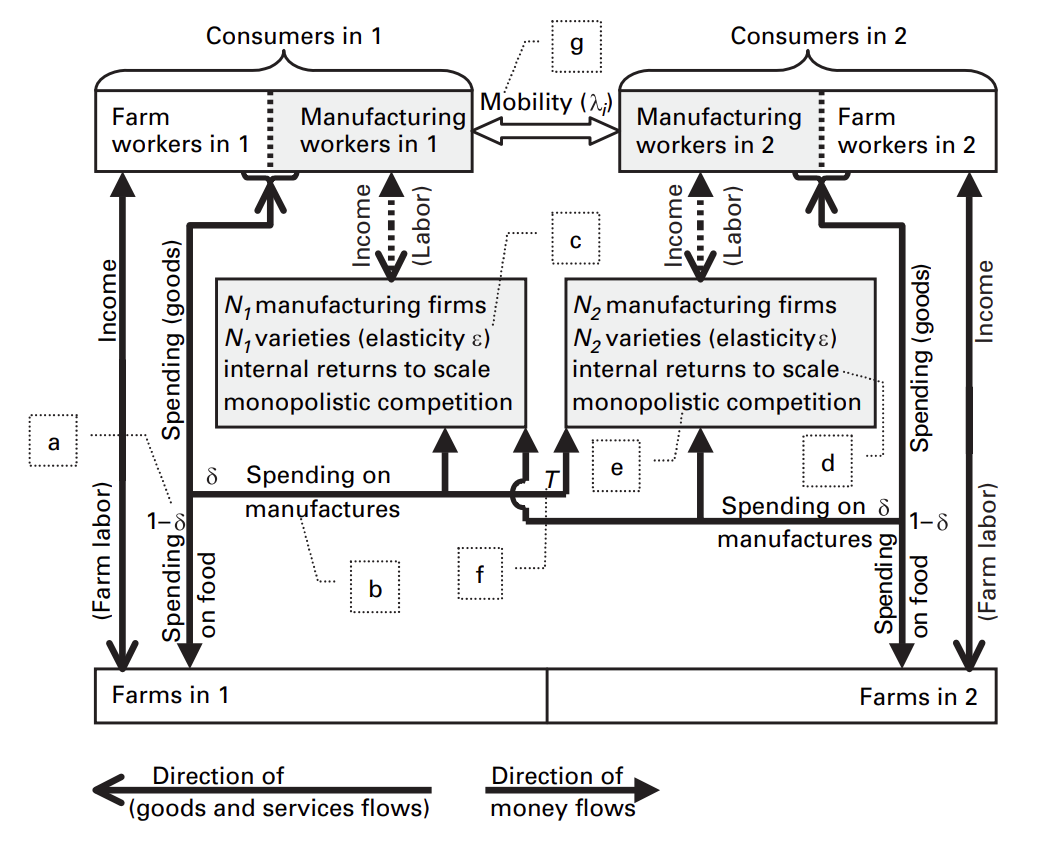
\includegraphics[scale=.3]{./imagen/diag.png}
\end{center}

\nbvspace[3]
\normalsize

LIBRO EN SU SEGUNDA EDICIÓN (Ingles)\\
\large
\nbvspace[1]

\end{center}

\break
\bfseries 

\nbvspace[1]
Título de la obra original:\\
THE NEW INTRODUCTION TO GEOGRAPHICAL ECONOMICS\\
Published in the United States of America by Cambridge University Press, New York\\

\nbvspace[1]

\begin{center}
Sin ninguna revisión de esta obra.\\


\nbvspace[1]
    Propiedad de esta obra:\\ 

    CHRISTIAN LIMBERT PAREDES AGUILERA\\	

    E-mail: soyfode@gmail.com
\end{center}

\nbvspace[1]

Reservados todos los derechos. La reproducción total o parcial de esta obra, por cualquier medio o procedimiento, comprendidos la reprografía y el tratamiento informático, y la distribución de ejemplares de ella mediante alquiler o préstamo públicos, queda rigurosamente prohibida sin la autorización escrita de los titulares del copyright, bajo las sanciones establecidas por las leyes.\\

\center 2022 

\end{titlingpage}


\pagenumbering{roman}

\tableofcontents								%indice

\pagestyle{fancy}
\fancyhead[LE,RO]{\nouppercase{\truncate{0.5\headwidth}{\rightmark}}}
\fancyhead[LO,RE]{\nouppercase{\truncate{0.5\headwidth}{\leftmark}}}



    %-------------------- Pensamiento economico -------------------
	%---------tareas
	    %\textbf{Christian Limbert Paredes Aguilera}\\
\textbf{Pensamiento Económico}\\\\
\begin{center}
\textbf{\Large Crecimiento y libertad económica: Un análisis cuantitativo}\\
\end{center}
\vspace{1cm}

    \section*{Introducción}
    Este trabajo tiene el propósito de analizar cuantitativamente la relación que existe entre el crecimiento económico y la libertad económica, por lo que recogeremos y organizaremos datos del instituto Fraser, del Penn World Table, de programad de desarrollo de las naciones unidas, de la universidad de Yale y del Banco Mundial. Dicho análisis se realizará para 112 países con el método de regresión de convergencia mediante  el entorno y lenguaje de programación R.\\
    El objetivo principal del modelo es, por un lado, ver si se cumple la convergencia del modelo de Solow donde los países que partían de un menor PIB pc tenían un crecimiento más rápido que los que partían de un PIB pc mayor y, por otro lado, analizar las variables de las que se componen la libertad económica y ver como se correlacionan con el crecimiento económico.

    \section*{Análisis descriptivo del índice de libertad económica y sus componentes}

    Libertad económica significa el grado en que existe una economía de mercado, donde los componentes centrales son el intercambio voluntario, la libre competencia y la protección de las personas y la propiedad (Gwartney y Lawson 2002, 5). El objetivo es caracterizar la estructura institucional y las partes centrales de la política económica. La libertad económica puede constituir un factor explicativo del crecimiento y de la distribución del ingreso. En el análisis econométrico, la libertad económica es, por tanto, una variable independiente. Sin embargo, la libertad económica también puede verse afectada por otras variables y, por lo tanto, constituir una variable dependiente, posiblemente influenciada por factores como la libertad política, la riqueza o la democracia.\\

    El intento más ambicioso de cuantificar la libertad económica es el Índice de Libertad Económica (EFI) que se informa anualmente en Economic Freedom of the World (Gwartney y Lawson 2002). Desde 1996, se han publicado datos actualizados anualmente, y los datos ahora cubren los años 1970, 1975, 1980, 1985, 1990, 1995 y 2000. Estos datos han comenzado a usarse en investigaciones académicas, que ha contribuido a aumentar nuestro conocimiento sobre la importancia de la libertad económica.\\
    Otro índice de este tipo es publicado por la Heritage Foundation en cooperación con el Wall Street Journal (O'Driscoll, Holmes y O'Grady 2002).3 Este índice y el EFI son similares en sus implicaciones generales, pero debido a que se ha utilizado el EFI más extensamente en contextos académicos.

    \subsection*{El concepto de libertad económica}
    La libertad económica es un compuesto que intenta caracterizar el grado en que una economía es una economía de mercado, es decir, el grado en el que implica la posibilidad de celebrar contratos voluntarios dentro del marco de un estado de derecho estable y predecible que respeta los contratos. Y protege la propiedad privada, con un grado limitado de intervencionismo en forma de propiedad del gobierno, regulaciones e impuestos. 
    El EFI es un medio de medir el grado de libertad económica al incluir treinta y siete componentes divididos en cinco grupos en un índice para los años, 1990 (113 países), 1995 (123 países) y 2000 (123 países). Los cinco grupos son: 

    \begin{enumerate}

	\item[Área 1.] \textbf{Tamaño del gobierno}.- A medida que aumentan el gasto público, los impuestos y el tamaño de las empresas controladas por el gobierno, la toma de decisiones del gobierno sustituye a la elección individual y se reduce la libertad económica.

	\item[Área 2.] \textbf{Sistema legal y derechos de propiedad}.- La protección de las personas y su propiedad legítimamente adquirida es un elemento central tanto de la libertad económica como de la sociedad civil. De hecho, es la función más importante del gobierno.

	\item[Área 3.] \textbf{La inflación monetaria sólida}.- erosiona el valor de los salarios y ahorros ganados legítimamente. Por lo tanto, el dinero sólido es esencial para proteger los derechos de propiedad. Cuando la inflación no solo es alta sino también volátil, se vuelve difícil para las personas planificar el futuro y, por lo tanto, utilizar la libertad económica de manera eficaz.

	\item[Área 4.] \textbf{Libertad para comerciar internacionalmente}.- La libertad para intercambiar —en su sentido más amplio, comprar, vender, hacer contratos, etc., es esencial para la libertad económica, que se reduce cuando la libertad de intercambiar no incluye empresas e individuos de otras naciones.

	\item[Área 5.] \textbf{Regulación}.- Los gobiernos no solo usan una serie de herramientas para limitar el derecho a intercambiar internacionalmente, sino que también pueden imponer regulaciones onerosas que limitan el derecho a intercambiar, obtener crédito, contratar o trabajar para quien usted desee u operar libremente su negocio.

    \end{enumerate}

    Cada componente se mide de 0 (sin libertad económica) a 10 o 100 (plena libertad económica). El índice se calcula utilizando promedios aritméticos.\\

    \begin{center}
	Tabla 1: Libertad económica\\(2017)\\
	\begin{tabular}{r|c}
	    \hline
	    \textbf{País} & \textbf{Indice} \\
	    \hline
	    Hong Kong & 89.8 \\
	    Estonia & 79.1 \\
	    Israeil & 69.7 \\
	    Burkina Faso & 59.6 \\
	    Mozambique & 49.9 \\
	    Venezuela & 27.0 \\
	    \hline
	\end{tabular}\\
	\small{Fuente: propia}
    \end{center}
    \vspace{.5cm}

    La Tabla de arriba presenta los valores de EFI en 2017 para varios países, en sus distintas categorías. En números absolutos, un pequeño país asiático junto con Estonia ocupan los puestos de arria. Al fondo, se encuentra Venezuela; varias naciones africanas también ocupan puestos bajos, tal es caso de Burkina Faso o Mozambique.\\


    \begin{center}
	Tabla 2: Libertad económica para EEUU.\\
	(1970-2000)\\
	\begin{tabular}{cccccccc}
	    \hline
	    Año&Rank&EFI&Gobierno&Legal&Moneda&Comercio&Regulación\\
	    \hline
	    1970&11&7.0&4.0&8.3&9.6&7.0&5.9\\
	    1975&3&7.3&4.8&7.9&9.2&7.7&6.7\\
	    1980&4&7.5&5.2&8.3&9.2&8.0&6.8\\
	    1985&5&7.7&6.0&8.3&9.3&7.8&6.8\\
	    1990&3&7.9&6.8&8.3&9.6&7.8&6.8\\
	    1995&4&8.3&6.9&8.6&9.7&7.9&8.3\\
	    2000&3&8.5&7.6&9.2&9.7&8.0&8.2\\
	    \hline
	\end{tabular}\\
	\small{Fuente: Gwartney and Lawson 2002, 165}
    \end{center}

    En la tabla 2 se presentan datos más detallados para los Estados Unidos. Los puntajes de los Estados Unidos son altos en todos los ámbitos. Se han realizado mejoras en todas las áreas durante el período estudiado, especialmente con respecto al tamaño del gobierno. El índice permite a los investigadores realizar análisis estadísticos de la importancia de la libertad económica. Al examinar la construcción del índice, se encuentra que se basa en gran parte en datos publicados en fuentes secundarias, que por lo tanto pueden verificarse fácilmente. Además, es fácil asignar nuevos pesos a los componentes del índice si así se desea.\\

    \subsection*{La importancia de la libertad económica}
    En la medida en que las instituciones estimulen acciones que contribuyan a la producción de productos más valiosos, contribuirán al crecimiento económico. Las instituciones que garantizan la libertad económica plausiblemente tienen la capacidad de proporcionar el tipo de incentivos que mejoran el crecimiento, por varias razones: promueven un alto rendimiento de los esfuerzos productivos a través de impuestos bajos, un sistema legal independiente y la protección de la propiedad privada; permiten que el talento se asigne donde genera el valor más alto (como se argumenta en Murphy, Schleifer y Vishny 1991); fomentan una economía dinámica, organizada experimentalmente, en la que puede tener lugar una gran cantidad de ensayo y error comercial (Johansson 2001, cap. 2) y en la que se produce competencia entre diferentes actores porque las regulaciones y las empresas gubernamentales son pocas; facilitan la toma de decisiones predecibles y racionales a través de una tasa de inflación baja y estable; y promueven el flujo de comercio e inversión de capital hacia donde la satisfacción de preferencias y los rendimientos son más altos.\\

    No es difícil afirmar que es probable que la libertad económica tenga un efecto favorable en la prosperidad económica, por la sencilla razón de que los últimos cincuenta años de experiencia internacional confirman más o menos el hecho de que dondequiera que los gobiernos usaron más los mercados y adoptaron políticas más abiertas en el comercio exterior y la inversión, de hecho en más libertad económica de diferentes tipos, sus países han tendido a prosperar. Por el contrario, aquellos países que se volvieron hacia adentro y tenían regulaciones extensas de todo tipo sobre la toma de decisiones económicas internas en producción, inversión e innovación, son los países que realmente no lo han hecho demasiado bien.\\

    \begin{center}
	Figura 1: Libertad económica y crecimiento del PIB per cápita.\\
	1990-2000\\
	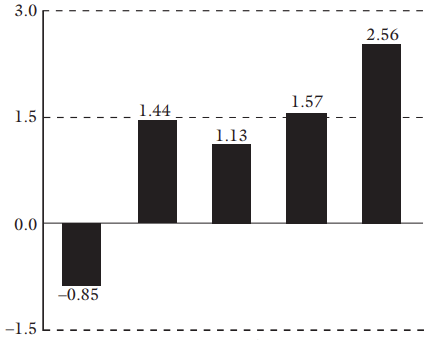
\includegraphics[scale=.5]{codigoFuente/tareas/pensamiento/img/1pensamiento.png}\\
	Quantiles EFI\\
	\small{Fuente: Gwartney and Lawson 2002,20}
    \end{center}

    Como muestra la figura, la quinta parte de los países que han tenido la libertad económica más alta han crecido considerablemente más rápido que otros países, mientras que la quinta parte de los países con la libertad económica más baja han tenido, de hecho, un crecimiento negativo. \\
    Gwartney, Lawson y Holcombe (1999), encuentran que el nivel de libertad económica al comienzo del período de crecimiento estudiado no contribuye significativamente explicar el crecimiento, pero que los cambios positivos en la libertad económica sí lo hacen. Por otro lado se encontró que el nivel inicial de libertad económica está positivamente relacionado con el crecimiento (Ali 1997; Easton y Walker 1997; Goldsmith 1997; Dawson 1998; Wu y Davis 1999; Hanson 2000; Heckelman y Stroup 2000;10Ali y Crain 2001 , 2002; Carlsson y Lundström 2002; Pitlik 2002; Scully 2002; Weede y Kämpf 2002). En varios de estos casos el efecto de nivel parece estadísticamente significativo solo si el cambio en la libertad económica también se incluye como variable.\\

    Algunas partes del EFI pueden promover el crecimiento más que otras. Carlsson y Lundström (2002) establecen que de los siete grupos EFI (en la versión publicada en 2000), cuatro se relacionan positiva y estadísticamente significativamente con el crecimiento (estructura económica y uso de mercados, libertad de uso de monedas alternativas, estructura legal y seguridad de propiedad y la libertad de intercambio en los mercados de capital), dos están negativamente y estadísticamente significativamente relacionados con el crecimiento (el tamaño del gobierno y el intercambio internacional/libertad para comerciar con extranjeros), y uno no está estadísticamente relacionado con el crecimiento (política monetaria y precios. Estabilidad). Lo más sorprendente de estos resultados, tanto desde una perspectiva teórica como en comparación con otros resultados empíricos, son las dos relaciones negativas detectadas. Implican que cuanto menor sea el tamaño del gobierno y mayor la libertad para comerciar con extranjeros, más lenta será la tasa de crecimiento. Una dificultad con las mediciones agregadas de este tipo es que ciertas empresas públicas pueden tener efectos de crecimiento positivos, mientras que otras tienen efectos negativos. 
    Otros estudios analizan el crecimiento o producto interno bruto (PIB) per cápita en función de la libertad económica o sus componentes. En general, los resultados son compatibles con los mencionados anteriormente, y aquí se presenta una selección de estos estudios.\\

    Los resultados más importantes se resumen en el cuadro 3. No se han informado resultados que muestren que la libertad económica obstaculiza el crecimiento o que está asociada con un PIB per cápita más bajo. Por el contrario, los resultados en general muestran que un aumento de la libertad económica ejerce una influencia positiva en el desarrollo de la riqueza económica.\\

    \begin{center}
	Tabla 3: El efecto de la libertad económica en el crecimiento y el PIB per capita
	\begin{tabular}{lccc}
	    \hline
	    Estudios & Variable dependiente & Variable independiente & Efecto \\
	    \hline
	    Dawson 1998, forthcoming,&&&\\
		     Gwartney, Lawson, y&Crecimiento&Cambio en la EFI&Significativa\\
					Holcombe 1999, de Hann&&&positivo\\
					y Sturn 2000,2001;&&&\\
					Adkins, Moomaw, y&&&\\
					Savvides 2002; Pitlik 2002;&&&\\
								   Weede y Kampf 2002&&&\\
												  \hline
										     Gwartney, Lawson y &Crecimiento&Nivel de la EFI&No\\
										     Holcombe 1999; de Hann y&&&significativo\\
										     Sturm 2000, 2001;&&&\\
										     Heckelman y Stroup 2000;&&&\\
										     Adkins, Moomaw, y&&&\\
										     Savvides 2002&&&\\
												  \hline
												  Ali 1997; Easton y Walker&Crecimiento&Nivel de la EFI&Significativo, \\
												  1997; Goldsmith 1997;&&&positivo\\
												  Dawson 1998, forthcoming;&&&\\
												  Wu y Davis 1999; Hanson&&&\\
												  2000; Ali y Crain 2001;&&&\\
												  2000; Carlsson and Lundstrom&&&\\
												  2002; Pitlik 2002; Scully&&&\\
												  2002; Weede y Kampf 2002&&&\\
												  \hline
							    Hanke y Walters 1997;&PIB&Nivel de la EFI&Significativo,\\
							    Leschke 2000&per capita&&positivo\\
							    \hline
							    Heckelman y Stroup 2000&Crecimiento&Nivel de una versión de la&Significativo,\\
							    &&EFI con diferentes valores&positivo\\
							    \hline
							    DE Vannsay y Spindler&Crecimiento&Nivel de indice de libertad&Significativo,\\
							    &&económica Scully-Slottje&positivo\\
							    \hline
							    De Haan y Siermann 1996,&Crecimiento&Nivel de indice de libertad&Resultado\\
							    1998&&económica Scully-Slottje&mezclado\\
							    \hline
	\end{tabular}\\
    \end{center}

    \subsection*{Igualdad de ingresos}
    Por un lado, la libertad económica está negativamente relacionada con la igualdad de ingresos, en un sentido estático (es decir, si uno observa el efecto parcial e inmediato de un cambio de política) y si la medida del ingreso son los ingresos disponibles (porque los impuestos y se puede esperar que los gastos de asistencia social generalmente asociados con una mayor libertad económica reduzcan la posición relativa de los asalariados de bajos ingresos). Por otro lado, los aumentos en la libertad económica afectan positivamente el crecimiento de los ingresos brutos, y si los grupos de bajos ingresos tienen una tasa de crecimiento más alta que otros como resultado de una mayor libertad económica, la distribución del ingreso puede ser más equitativa.\\
    Un mapeo simple de Gwartney y Lawson (2002) muestra que no parece existir una relación clara entre la libertad económica y la situación relativa de los más pobres, como se desprende del gráfico 2.\\

    \begin{center}
	Figura 2: La libertad económica y la participación \\ en el ingreso del 10 por ciento más pobre.\\
	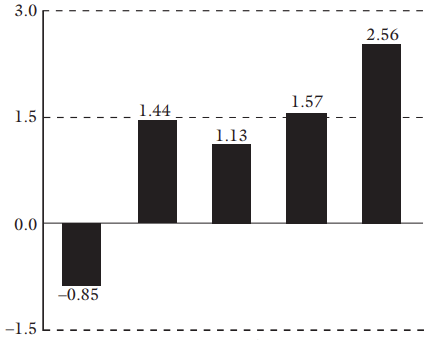
\includegraphics[scale=.5]{codigoFuente/tareas/pensamiento/img/1pensamiento.png}\\
	Quantiles EFI\\
	\small{Fuente: Gwartney y Lawson 2002,20}
    \end{center}

    Berggren (1999) encuentra que cuanto más aumentaba la libertad económica en un país entre 1975 y 1985, mayor era el grado de igualdad de ingresos de ese país alrededor de 1985. En particular, este resultado es válido para los países en desarrollo y para el momento en que se produjeron los cambios de política. liberalizó el comercio y desreguló el sistema financiero. La igualdad se mide como coeficientes de Gini y como comparaciones entre la participación en el ingreso o el consumo de personas con ingresos bajos y altos. Al mismo tiempo, el nivel de libertad económica en 1985 parece tener una relación negativa con la igualdad de ingresos, lo que probablemente sea un efecto de la redistribución reducida. Grubel (1998) da la vuelta al problema y estudia cómo la igualdad de ingresos afecta el PIB per cápita, el crecimiento económico y la libertad económica en diecisiete países con un PIB per cápita superior a 17.000 dólares. Los resultados sugieren que una mayor igualdad de ingresos está relacionada con un menor PIB per cápita, menor crecimiento y menor libertad económica. Scully (2002) estima un modelo estructural y modelos de forma reducida y muestra que la libertad económica es beneficiosa tanto para el crecimiento económico como para la igualdad porque tiene un efecto negativo significativo en los coeficientes de Gini. Además, una mayor igualdad reduce el crecimiento, pero solo en una pequeña cantidad.

    \section*{La libertad económica en contexto}
    Analizaremos la relación entre la libertad económica y otras variables tales como el PIB per cápita, el capital humano, el índice de desarrollo humano, el índice de desempeño ambiental, indice de Gini y el desempleo total.\\
    Para ello elaboramos y mostramos un gráfico multiple extraída de las distintas fuentes de datos para el año 2017 el cual se detalla a continuación. 


    \begin{center}
	Figura 3: Libertad económica en contexto.\\
	2017\\
	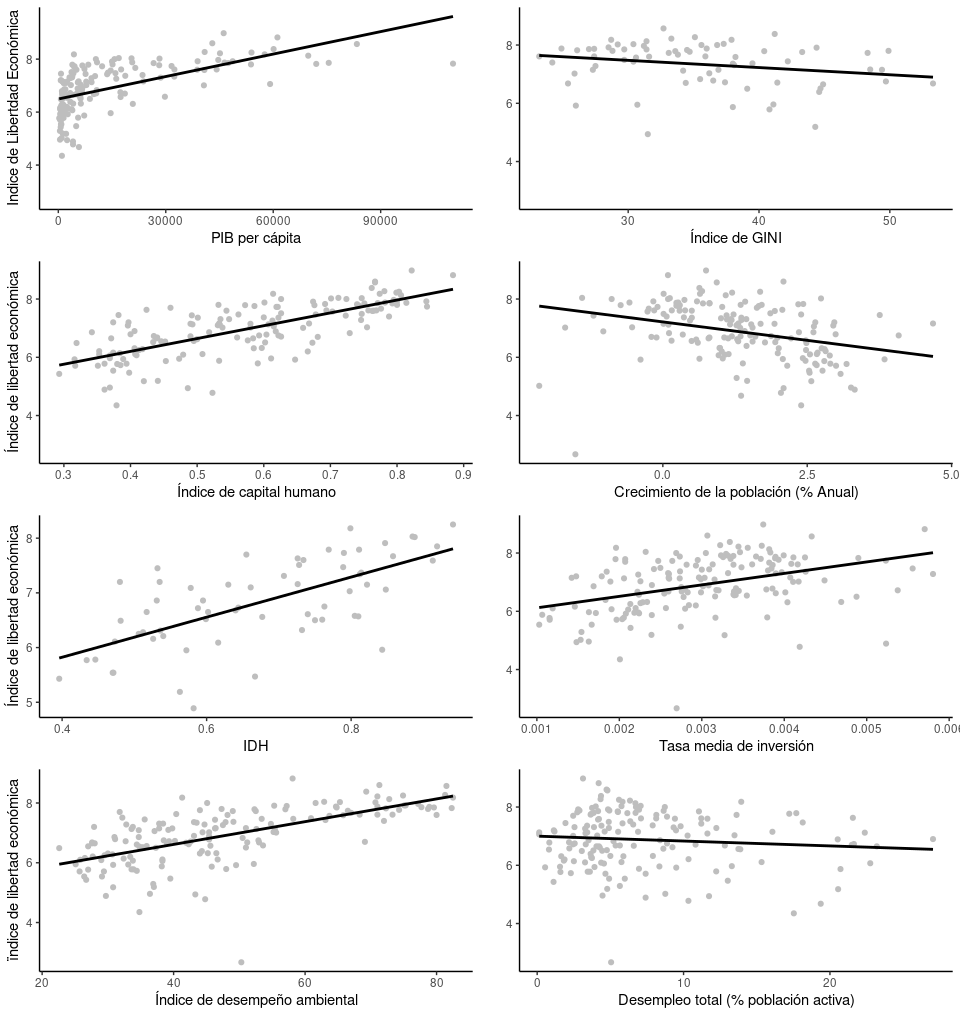
\includegraphics[scale=.65]{codigoFuente/tareas/pensamiento/img/multiplot.png}

	\small{Fuente: Banco Mundial y Universidad de Yale.}
    \end{center}

	\textbf{Relación con el PIB per cápita.}
	Como vimos en el anterior apartado la relación que existe entre la libertad económica y el PIB per cápita esta directamente o positivamente relacionado. Esto lo confirma la primera relación de la izquierda del gráfico 3. Donde a mayor puntuación en el índice se tendrá un PIB per cápita superior, es otras palabras a mayor PIB per cápita cualquier país recibirá una mejor puntación en el ranking. Esto se ve más clara si trazamos una linea de tendencia.\\\\

	\textbf{Relación con el capital humano.}
	Lo propio pasa cuando relacionamos la libertad económica y el capital humano. Como bien sabemos el capital humano es la parte más importante de cualquier organización el cual hace referencia a la productividad de los trabajadores que depende de su experiencia laboral y de su formación. Dicho un país goza de mayor libertad económica si la productividad de los trabajadores es mayor y mejor.\\\\

	\textbf{Relación con el índice de desarrollo humano.}
	A diferencia del capital humano en si, el índice de desarrollo humano se enfoca en tratar de promocionar el desarrollo potencial de las personas, el aumento de sus posibilidades, y el disfrute de la libertad para vivir la vida que valoran. Sabiendo este último y mostrado claramente en la parte inferior izquierda de la figura 3, vemos claramente una pendiente cerca de 1, el cual nos confirma que la libertad económica está positivamente correlacionada con la libertad para vivir, es decir, mayor IDH sugiere mayor libertad económica. \\\\


	\textbf{Relación con el índice de desempeño ambiental.}
	El Índice de Desempeño Ambiental (EPI por sus siglas en inglés: Environmental Performance Index), clasifica los países a partir de su desempeño en el logro de dos objetivos ambientales prioritarios: la salud ambiental que mide la protección de la salud humana ante el impacto de los daños ambientales; y la vitalidad de los ecosistemas que mide la protección a los ecosistemas y la administración de recursos. Este método para cuantificar y clasificar numéricamente el desempeño ambiental de las políticas de un país, esta claramente relaciono con la libertad económica, así se ve en el gráfico 3 en la parte superior derecha. A mejor puntación en el desempeño ambiental de un país, más libertad económica del mismo. A primera vista podría parecer ilógico esta afirmación pero la explicación partiría por el hecho de que a mayor libertad económica mayor políticas ambientales en un país.\\\\
	    
	\textbf{Relación con la Desigualdad y la distribución de la riqueza.}
	Para medir la desigualdad entre los habitantes de una población hacemos uso de la herramienta denominada indice de Gini. Este representa la desigualdad máxima que la cuantificamos con el número 1 o el 100, en cuyo caso uno solo de los habitantes recibiría el total de los ingresos por salarios. Por otro lado el 0, significa la igualdad total de los ingresos salariales de todos los habitantes. En este caso y según la gráfica 3 vemos que el índice de Gini esta negativamente relacionada con la libertad económica, en otras palabras podemos decir que mientras más desigualdad se tiene en un país más libertad económica existe.\\\\

	\textbf{Relación con el crecimiento de la población.}
	El crecimiento de una población se refiere, simplemente, al aumento, disminución o estabilidad en el número de sus integrantes en cada país, que ocurre en un período de tiempo determinado. Por lo que  vemos que a medida que el porcentaje de población anual aumenta entonces disminuye la libertad económica, por lo que nos muestra una pendiente ligeramente negativa.\\\\
    

	\textbf{Relación con la tasa media de inversión.}
	La tasa media de inversión prácticamente mide en cuanto ha crecido una inversión en un período determinado de tiempo. En este caso para el periodo de 2017 tenemos una relación positiva con respecto a la libertad económica, por lo que a medida que crece la tasa media de inversión también crecerá la libertad económica.\\\\

	\textbf{Relación con el desempleo.}
	El desempleo total de la población activa juega un rol interesante a la hora de relacionarse con la libertad económica de un país.\\
	Revisando la gráfica 3 en la parte inferior derecha, vemos que se tiene una ligera inclinación negativa entre el desempleo de un país y la libertad económica. Nos menciona que a mayor desempleo menor libertad económica y lo contrario a menor desempleo mayor libertad económica.  


\section*{La libertad económica y el crecimiento económico}
Una primera hipótesis propuesta por historiadores económicos como Aleksander Gerschenkron (1952) y MOses Abramovitz (1986) fue, que al menos en ciertas circunstancias, los países atrasados tenderían a crecer con más rapidez que los países ricos, este fenómeno se conoce como convergencia. A esto y con alguna investigación empírica llegamos a la conclusión de que algunos grupos de países si cumplen con la hipótesis dada y no así todo el conjunto de países del mundo. La pregunta es ¿Por qué? Para ello nos basamos en el modelo negoclásico.\\
Observemos la ecuación diferencial clave del modelo de crecimiento neoclásico,
$$\tilde{k}=s_K \tilde{y}-(n+g+d)\tilde{k}$$
Esta ecuación se puede escribir de nuevo como,
$$\dfrac{\tilde{k}}{\tilde{k}}=s_K \dfrac{\tilde{y}}{\tilde{k}}-(n+g+d)$$
Dónde podemos deducir que el producto promedio del capital disminuye según aumenta k debido a la acumulación de los rendimientos decrecientes de capital en el modelo neoclásico. Luego sabemos que la tasa de crecimiento de la tecnología es constante por lo que cualquier cambio de las tasas de crecimiento de $k$ e $y$ se debe atribuir a cambios en las tasas de crecimiento del capital por trabajador y de la producción por trabajador. Asi sacamos dos supuestos:
\begin{enumerate}
    \item Entre países que tienen el mismo estado estacionario, debe cumplirse la hipótesis de la convergencia: los países pobres deben crecer con mayor rapidez, en promedio, que los ricos.
    \item Principio de la dinámica de transición. Cuanto más se encuentre una economía por debajo de su estado estacionario con mayor rapidez deberá crecer y cuanto más por encima esté con mayor lentitud deberá crecer.
\end{enumerate}
Finalmente, la teoría de convergencia condicional se puede contrastar regresando la tasa de crecimiento del PIB pc, contra el logaritmo del PIB inicial y condicionando la regresión por las variables determinantes del estado estacionario,

$$\dfrac{1}{T}\ln\dfrac{Y_t}{Y_0}=B_0+B_1\ln Y_0 + B_2 X_2 + B_3 X_3 + \ldots + B_i X_i$$

Ya representados la tasa de crecimiento y el logaritmo de PIB per cápita inicial condicionado por las diferentes variables que determinan el PIB per cápita en el estado estacionario destacando que dentro de estas variables se encuentra la libertad económica y las diferentes variables explicativas del Instituto Fraser, además de otras variables que determinan el desempeño económico de un país a largo plazo, podremos realizar las distintas regresiones de convergencia.\\\\
Para tal efecto tendremos en cuenta la muestra de 112 países y algunos periodos de tiempo como los periodos de 1990-2017, 1990-2000, 2001-2007, 1990-2007 y 2008-2017. \\\\
La variable dependiente estará dada por:

\begin{center}
$PIBpc = \dfrac{1}{T}\ln\dfrac{Y_t}{Y_0}=y$ = tasa de crecimiento del PIB per cápita.

\end{center}

Las variables explicativas estarán dadas por: 

\begin{center}
\begin{tabular}{rcl}
    $lny_0$&=&Logaritmo del PIB per cápita inicial\\
    $ile_i$&=&Indice de libertad económica para el año final.\\
    $ile_0$&=&Índice de libertad económica inicial.\\
    $ tc_i$&=&Tasa de cambio del índice de libertad económica en el año final.\\
    $ich_i$&=&Índice de capital humano por trabajador en el año final.\\
    $tmi$&=&Tasa media de inversión de cada país durante el periodo de análisis.\\
    $n=tpob$&=&Tasa anual media de crecimiento de la población durante el periodo de análisis.\\
    $a1$&=&Área 1. Tamaño de gobierno.\\
    $a2$&=&Área 2. Sistema legal y derechos de propiedad.\\
    $a3$&=&Área 3. Moneada sólida.\\
    $a4$&=&Área 4. Libertad para comerciar internacionalmente.\\
    $a5$&=&Área 5. Regulación.\\
    $va$&=&Índice de calidad de gobernanza voice and Accountability.\\
    $PS=sav$&=&Índice de calidad de gobernanza Political Stability and Absence of Violence.\\\\
\end{tabular}
\end{center}

\subsection*{Regresiones de convergencia}
Para estas regresiones de convergencia analizaremos varios modelos con distintas variables explicativas.\\
\begin{enumerate}[\bfseries 1.]
   \item Primeramente utilizaremos las variables: valor del índice de libertad económica en el año inicial y el año final, donde introduciremos y sacaremos ambos de la regresión para ver cual es el que ayuda a explicar la tasa de crecimiento.
	$$\begin{array}{rcl}
	    y&=&\beta_0 + \beta_1\cdot lny_0 + \beta_2\cdot ile_i + \beta_3\cdot ile_0 + \beta_4\cdot tc_i + \beta_5\cdot ich_i + \beta_6\cdot tmi + \beta_7\cdot tpob + \epsilon\\\\
	    y&=&\beta_0 + \beta_1\cdot lny_0 + \beta_4\cdot tc_i + \beta_5\cdot ich_i + \beta_6\cdot tmi + \beta_7\cdot tpob + \epsilon\\\\
	\end{array}$$

    \item Probar introduciendo y sacando la tasa de cambio de índice de libertad económica para el año final con el objetivo de ver su poder explicativo.

	$$\begin{array}{rcl}
	    y&=&\beta_0 + \beta_1\cdot lny_0 + \beta_2\cdot ile_i + \beta_3\cdot ile_0 + \beta_4\cdot tc_i +\beta_5\cdot ich_i + \beta_6\cdot tmi + \beta_7\cdot tpob + \epsilon$$\\\\
	    y&=&\beta_0 + \beta_1\cdot lny_0 + \beta_2\cdot ile_i + \beta_3\cdot ile_0 + \beta_5\cdot ich_i + \beta_6\cdot tmi + \beta_7\cdot tpob + \epsilon$$\\\\
	\end{array}$$

    \item Probaremos  introduciendo diferentes componentes del índice de libertad económica para ver su capacidad explicativa de igual modo que hemos hecho con el índice agregado.

	$$\begin{array}{rcl}
	    y&=&\beta_0 + \beta_1\cdot lny_0 + \beta_5\cdot ich_i + \beta_6\cdot tmi + \beta_7\cdot tpob + \beta_{a1}\cdot a1 + \beta_{a2}\cdot a2  + \beta_{a3}\cdot a3 + \beta_{a4}\cdot a4 + \beta_{a5}\cdot a5 + \epsilon\\\\
	    y&=&\beta_0 + \beta_1\cdot lny_0 + \beta_5\cdot ich_i + \beta_6\cdot tmi + \beta_7\cdot tpob + \beta_{a1}\cdot a1 + \epsilon\\\\
	    y&=&\beta_0 + \beta_1\cdot lny_0 + \beta_5\cdot ich_i + \beta_6\cdot tmi + \beta_7\cdot tpob + \beta_{a2}\cdot a2 + \epsilon\\\\
	    y&=&\beta_0 + \beta_1\cdot lny_0 + \beta_5\cdot ich_i + \beta_6\cdot tmi + \beta_7\cdot tpob  + \beta_{a3}\cdot a3 + \epsilon\\\\
	    y&=&\beta_0 + \beta_1\cdot lny_0 + \beta_5\cdot ich_i + \beta_6\cdot tmi + \beta_7\cdot tpob + \beta_{a4}\cdot a4 + \epsilon\\\\
	    y&=&\beta_0 + \beta_1\cdot lny_0 + \beta_5\cdot ich_i + \beta_6\cdot tmi + \beta_7\cdot tpob + \beta_{a5}\cdot a5 + \epsilon\\\\
	\end{array}$$

    \item Por último Introduciremos como variables explicativas los índices de calidad de gobernanza Voice and Accountability y Political Stability and Absence of Violence elaborados por el Banco Mundial. Tomaremos el valor del último año del periodo de análisis.
	$$\begin{array}{rcl}
	    y&=&\beta_0 + \beta_1\cdot lny_0 + \beta_2\cdot ile_i + \beta_3\cdot ile_0 + \beta_4\cdot tc_i + \beta_5\cdot ich_i + \beta_6\cdot tmi + \beta_7\cdot tpob + \beta_{g1}\cdot va + \beta_{g2}\cdot sav + \epsilon\\\\
	    y&=&\beta_0 + \beta_1\cdot lny_0 + \beta_2\cdot ile_i + \beta_3\cdot ile_0 + \beta_4\cdot tc_i + \beta_5\cdot ich_i + \beta_6\cdot tmi + \beta_7\cdot tpob + \beta_{g1}\cdot va + \epsilon\\\\
	    y&=&\beta_0 + \beta_1\cdot lny_0 + \beta_2\cdot ile_i + \beta_3\cdot ile_0 + \beta_4\cdot tc_i + \beta_5\cdot ich_i + \beta_6\cdot tmi + \beta_7\cdot tpob + \beta_{g2}\cdot sav + \epsilon\\\\
	\end{array}$$

\end{enumerate}

	    \subsubsection*{Periodo 1990-2017}

		Según el cuadro 1 (Apéndice), vemos que los índices de libertad económica para el año inicial y final, explican a la tasa de crecimiento del PIB per cápita, esto, porque estás son significativas al $1\%$. Por el contrario y curiosamente, cuando obviamos las mismas, observamos que las demás variables como ser la tasa de cambio del índice económico y tasa media de inversión tasa anual media de crecimiento de la población se vuelven significativas.\\
		Según el cuadro 2, el poder explicativo de la tasa de cambio del índice de libertad económica es indistinta. Es decir, sea o no se incluya esta variable el $R^2$ no variara, pero si lo hara el estadístico F, con un aumento si esta variable no se toma en cuenta.\\  
		Con respecto a los diferentes componentes del índice de libertad económica los que más podrían explicar a la tasa de crecimiento del Pib pc son el sistema legal y derecho de propiedad y libertad para comercializar internacionalmente, eso si con un $R^2$ muy bajo en todos los casos pero un estadístico F algo.\\
		Por último cuando introducimos los índices de calidad de gobernanza vemos que el que mejor explica es Estabilidad Política y Ausencia de Violencia. 

	    \subsubsection*{Periodo 1990-2000}

		Contrario al periodo 1990-2017 vemos que la única variable significativa para poder explicar la tasa de crecimiento del PIB pc es el índice de libertad económica para el año final (2000), pero con buenos resultados para las demás variables explicativas como ser el índice de capital humano, tasa media de inversión y la tasa anual media de crecimiento de la población.\\
		Un buen modelo para este periodo podría ser obviando la tasa de cambio del índice de libertad económica, pero inversamente proporcional para casi toda las variables explicativas.\\
		Con respecto a las diferentes componentes del índice de libertad económica vemos que ninguna de estas es significativa, pero cada modelo explica levemente mejor que las del periodo 1990-2017.\\
		De igual forma al anterior periodo, al introducir los índices de calidad de gobernanza la que mejor variable que explica a la tasa de crecimiento del PIB pc es la estabilidad política y ausencia de violencia en un país, pero con casi todas variables negativas.\\

	    \subsubsection*{Periodo 2001-2007}
		
		Para este periodo observamos que las variables de índice de libertad económica para el año inicial y final no son significativas por lo tanto no explican de buena manera a la tasa de crecimiento del PIB pc.(Cuadro 9)\\
		Con respecto a introducir la tasa de cambio del índice de libertad económica, podría tener un poder explicativo pero muy leve.\\
		Por otro lado cuando incluimos los diferentes componentes del índice de libertad económica vemos que el que mejor podría explicar a la variable independiente es el sistema legal y derecho de propiedad pero con un poder explicativo muy bajo.\\
		Luego, contrario a los periodos 1990-2017 y 1990-2000 la variable que mejor aporta a explicar al PIB al incluir los índices de calidad de gobernanza es Voice and Accountability, pero de manera negativa, y un $R^2$ bajo (cuadro 12).\\

	    \subsubsection*{Periodo 1990-2007}
	    
		Como en el periodo 1990-2017 vemos que al introducir las respectivas variables del índice de libertad económica para el año inicial y final podría ayudar a explicar a la tasa de crecimiento pero con una significancia del $10\%$ y un $R^2$ del 0.2 (cuadro 13). Cabe mencionar que la tasa de cambio del índice de libertad económica para este periodo no tiene alguna relevancia.\\
		Con respecto a los componentes del índice de libertad, como vimos a un principio, las variables que explican y son significativas son el sistema legal y la libertad para comercializar. No pasa lo mismo con los índices de calidad de gobernanza donde ninguna es apropiada para explicar a la tasa de crecimiento.


	    \subsubsection*{Periodo 2008-2017}

		Al agregar los índices de libertad económica observamos que no son significativas para el modelo, pero si lo es la tasa de cambio. Contrario a esto, cuando excluimos la tasa de cambio los índices de libertad económica se vuelve significativas al $1\%$ con un $R^2$ de $0.34$.\\
		Cuando probamos incluir las componentes del índice de libertad la única que parece significativa es la de libertad comercial pero con un bajo poder explicativo.\\
		Por último y con un grado muy aceptable de poder explicativo a los índices de calidad de gobernanza.



    \section*{Conclusiones}

    Al poder realizar las distintas regresiones de covergencia, podemos notar que a través del tiempo las distintas variables que explican ala tasa de crecimiento, entre las cuales se encuentra el índice de libertad económica, toman mas protagonismo, esto podría deberse a la mejora continua al adquirir los distintos datos.\\
    
    Luego, podemos concluir que las variables que hacen referencia al índice de libertad económica no son del todo significativas si usamos paralelamente en el modelo esto por motivos de significancia y correlación. Por lo que para obtener un modelo donde estas variables sean significativas, y estén correlacionadas tendremos que escoger un modelo el cual suprimiera una de estas dos mantuviera la tasa de cambio del índice.\\

    Por otro lado concluimos  que los componentes del índice de libertad económica no trabajan bien en si incluimos sólo un componente, ya que algunos no son significativos. Mientras que si serán significativos si las estudiamos en conjunto.\\

/bin/bash: :wq: orden no encontrada

\clearpage

    \section*{Apéndice}

%-------------------------------------------------------------------
%-----------------------------1-------------------------------------
\begin{table}[!htbp] \centering 
    \tiny
  \caption{} 
  \label{} 
\begin{tabular}{@{\extracolsep{5pt}}lcc} 
\\[-1.8ex]\hline 
\hline \\[-1.8ex] 
 & \multicolumn{2}{c}{\textit{Dependent variable:}} \\ 
\cline{2-3} 
\\[-1.8ex] & \multicolumn{2}{c}{y} \\ 
\\[-1.8ex] & (1) &(2)\\ 
\hline \\[-1.8ex] 
 lny\_0 & 0.001 & $-$0.0003 \\ 
  & p = 0.543 & p = 0.811 \\ 
  & & \\ 
 ile\_i & 0.018$^{***}$ &  \\ 
  & p = 0.001 &  \\ 
  & & \\ 
 ile\_0 & $-$0.012$^{**}$ &  \\ 
  & p = 0.037 &  \\ 
  & & \\ 
 tc\_i & $-$0.017 & 0.028$^{***}$ \\ 
  & p = 0.398 & p = 0.00003 \\ 
  & & \\ 
 ich\_i & $-$0.007 & $-$0.003 \\ 
  & p = 0.142 & p = 0.533 \\ 
  & & \\ 
 tmi & 0.050 & 0.083$^{**}$ \\ 
  & p = 0.147 & p = 0.021 \\ 
  & & \\ 
 tpob & $-$0.240 & $-$0.399$^{*}$ \\ 
  & p = 0.249 & p = 0.066 \\ 
  & & \\ 
 Constant & $-$0.007 & $-$0.014 \\ 
  & p = 0.809 & p = 0.468 \\ 
  & & \\ 
\hline \\[-1.8ex] 
Observations & 112 & 112 \\ 
R$^{2}$ & 0.324 & 0.219 \\ 
Adjusted R$^{2}$ & 0.278 & 0.182 \\ 
Residual Std. Error & 0.019 (df = 104) & 0.020 (df = 106) \\ 
F Statistic & 7.119$^{***}$ (df = 7; 104) & 5.952$^{***}$ (df = 5; 106) \\ 
\hline 
\hline \\[-1.8ex] 
\textit{Note:}  & \multicolumn{2}{r}{$^{*}$p$<$0.1; $^{**}$p$<$0.05; $^{***}$p$<$0.01} \\ 
\end{tabular} 
\end{table} 


\begin{table}[!htbp] \centering 
    \tiny
  \caption{} 
  \label{} 
\begin{tabular}{@{\extracolsep{5pt}}lcc} 
\\[-1.8ex]\hline 
\hline \\[-1.8ex] 
 & \multicolumn{2}{c}{\textit{Dependent variable:}} \\ 
\cline{2-3} 
\\[-1.8ex] & \multicolumn{2}{c}{y} \\ 
\\[-1.8ex] & (1) & (2)\\ 
\hline \\[-1.8ex] 
 lny\_0 & 0.001 & 0.0005 \\ 
  & p = 0.543 & p = 0.663 \\ 
  & & \\ 
 ile\_i & 0.018$^{***}$ & 0.014$^{***}$ \\ 
  & p = 0.001 & p = 0.00000 \\ 
  & & \\ 
 ile\_0 & $-$0.012$^{**}$ & $-$0.008$^{***}$ \\ 
  & p = 0.037 & p = 0.00003 \\ 
  & & \\ 
 tc\_i & $-$0.017 &  \\ 
  & p = 0.398 &  \\ 
  & & \\ 
 ich\_i & $-$0.007 & $-$0.008 \\ 
  & p = 0.142 & p = 0.103 \\ 
  & & \\ 
 tmi & 0.050 & 0.051 \\ 
  & p = 0.147 & p = 0.140 \\ 
  & & \\ 
 tpob & $-$0.240 & $-$0.269 \\ 
  & p = 0.249 & p = 0.192 \\ 
  & & \\ 
 Constant & $-$0.007 & $-$0.025 \\ 
  & p = 0.809 & p = 0.187 \\ 
  & & \\ 
\hline \\[-1.8ex] 
Observations & 112 & 112 \\ 
R$^{2}$ & 0.324 & 0.319 \\ 
Adjusted R$^{2}$ & 0.278 & 0.280 \\ 
Residual Std. Error & 0.019 (df = 104) & 0.019 (df = 105) \\ 
F Statistic & 7.119$^{***}$ (df = 7; 104) & 8.207$^{***}$ (df = 6; 105) \\ 
\hline 
\hline \\[-1.8ex] 
\textit{Note:}  & \multicolumn{2}{r}{$^{*}$p$<$0.1; $^{**}$p$<$0.05; $^{***}$p$<$0.01} \\ 
\end{tabular} 
\end{table} 


\begin{table}[!htbp] \centering 
    \tiny
  \caption{} 
  \label{} 
\begin{tabular}{@{\extracolsep{5pt}}lcccccc} 
\\[-1.8ex]\hline 
\hline \\[-1.8ex] 
 & \multicolumn{6}{c}{\textit{Dependent variable:}} \\ 
\cline{2-7} 
\\[-1.8ex] & \multicolumn{6}{c}{y} \\ 
\\[-1.8ex] & (1) & (2) &  (3) & (4) & (5) & (6)\\ 
\hline \\[-1.8ex] 
 lny\_0 & 0.0005 & $-$0.001 & $-$0.001 & $-$0.001 & 0.0003 & $-$0.001 \\ 
  & p = 0.738 & p = 0.640 & p = 0.595 & p = 0.690 & p = 0.834 & p = 0.557 \\ 
  & & & & & & \\ 
 ich\_i & 0.006 & $-$0.005 & 0.003 & $-$0.006 & 0.001 & $-$0.004 \\ 
  & p = 0.335 & p = 0.317 & p = 0.579 & p = 0.234 & p = 0.837 & p = 0.395 \\ 
  & & & & & & \\ 
 tmi & 0.095$^{**}$ & 0.072$^{*}$ & 0.099$^{**}$ & 0.078$^{**}$ & 0.090$^{**}$ & 0.077$^{**}$ \\ 
  & p = 0.019 & p = 0.060 & p = 0.011 & p = 0.046 & p = 0.023 & p = 0.048 \\ 
  & & & & & & \\ 
 tpob & $-$0.624$^{**}$ & $-$0.505$^{**}$ & $-$0.740$^{***}$ & $-$0.570$^{**}$ & $-$0.367 & $-$0.513$^{**}$ \\ 
  & p = 0.034 & p = 0.029 & p = 0.002 & p = 0.015 & p = 0.136 & p = 0.035 \\ 
  & & & & & & \\ 
 a1 & $-$0.002 & $-$0.001 &  &  &  &  \\ 
  & p = 0.310 & p = 0.409 &  &  &  &  \\ 
  & & & & & & \\ 
 a2 & $-$0.005$^{*}$ &  & $-$0.005$^{***}$ &  &  &  \\ 
  & p = 0.052 &  & p = 0.008 &  &  &  \\ 
  & & & & & & \\ 
 a3 & 0.0004 &  &  & $-$0.001 &  &  \\ 
  & p = 0.720 &  &  & p = 0.478 &  &  \\ 
  & & & & & & \\ 
 a4 & $-$0.002 &  &  &  & $-$0.003$^{***}$ &  \\ 
  & p = 0.117 &  &  &  & p = 0.005 &  \\ 
  & & & & & & \\ 
 a5 & 0.003 &  &  &  &  & $-$0.001 \\ 
  & p = 0.273 &  &  &  &  & p = 0.370 \\ 
  & & & & & & \\ 
 Constant & 0.024 & 0.042$^{**}$ & 0.038$^{**}$ & 0.040$^{**}$ & 0.021 & 0.042$^{**}$ \\ 
  & p = 0.264 & p = 0.025 & p = 0.019 & p = 0.017 & p = 0.233 & p = 0.013 \\ 
  & & & & & & \\ 
\hline \\[-1.8ex] 
Observations & 106 & 111 & 112 & 112 & 107 & 112 \\ 
R$^{2}$ & 0.170 & 0.082 & 0.138 & 0.083 & 0.142 & 0.086 \\ 
Adjusted R$^{2}$ & 0.092 & 0.039 & 0.098 & 0.040 & 0.100 & 0.043 \\ 
Residual Std. Error & 0.021 (df = 96) & 0.022 (df = 105) & 0.021 (df = 106) & 0.022 (df = 106) & 0.021 (df = 101) & 0.022 (df = 106) \\ 
F Statistic & 2.187$^{**}$ (df = 9; 96) & 1.881 (df = 5; 105) & 3.408$^{***}$ (df = 5; 106) & 1.924$^{*}$ (df = 5; 106) & 3.353$^{***}$ (df = 5; 101) & 1.990$^{*}$ (df = 5; 106) \\ 
\hline 
\hline \\[-1.8ex] 
\textit{Note:}  & \multicolumn{6}{r}{$^{*}$p$<$0.1; $^{**}$p$<$0.05; $^{***}$p$<$0.01} \\ 
\end{tabular} 
\end{table}




\begin{table}[!htbp] \centering 
    \tiny
  \caption{} 
  \label{} 
\begin{tabular}{@{\extracolsep{5pt}}lccc} 
\\[-1.8ex]\hline 
\hline \\[-1.8ex] 
 & \multicolumn{3}{c}{\textit{Dependent variable:}} \\ 
\cline{2-4} 
\\[-1.8ex] & \multicolumn{3}{c}{y} \\ 
\\[-1.8ex] & (1)  & (2) & (3)\\ 
\hline \\[-1.8ex] 
 lny\_0 & $-$0.001 & 0.0005 & $-$0.001 \\ 
  & p = 0.524 & p = 0.683 & p = 0.505 \\ 
  & & & \\ 
 ile\_i & 0.021$^{***}$ & 0.021$^{***}$ & 0.020$^{***}$ \\ 
  & p = 0.0003 & p = 0.0003 & p = 0.0002 \\ 
  & & & \\ 
 ile\_0 & $-$0.010$^{*}$ & $-$0.012$^{**}$ & $-$0.010$^{*}$ \\ 
  & p = 0.093 & p = 0.040 & p = 0.095 \\ 
  & & & \\ 
 tc\_i & $-$0.014 & $-$0.020 & $-$0.012 \\ 
  & p = 0.504 & p = 0.326 & p = 0.534 \\ 
  & & & \\ 
 ich\_i & $-$0.003 & $-$0.006 & $-$0.003 \\ 
  & p = 0.493 & p = 0.222 & p = 0.477 \\ 
  & & & \\ 
 tmi & 0.070$^{*}$ & 0.044 & 0.073$^{**}$ \\ 
  & p = 0.053 & p = 0.202 & p = 0.037 \\ 
  & & & \\ 
 tpob & $-$0.417$^{*}$ & $-$0.351 & $-$0.395$^{*}$ \\ 
  & p = 0.060 & p = 0.116 & p = 0.063 \\ 
  & & & \\ 
 va & $-$0.001 & $-$0.005 &  \\ 
  & p = 0.706 & p = 0.167 &  \\ 
  & & & \\ 
 sav & $-$0.009$^{**}$ &  & $-$0.009$^{***}$ \\ 
  & p = 0.026 &  & p = 0.010 \\ 
  & & & \\ 
 Constant & $-$0.039 & $-$0.018 & $-$0.037 \\ 
  & p = 0.203 & p = 0.542 & p = 0.213 \\ 
  & & & \\ 
\hline \\[-1.8ex] 
Observations & 112 & 112 & 112 \\ 
R$^{2}$ & 0.368 & 0.336 & 0.367 \\ 
Adjusted R$^{2}$ & 0.313 & 0.285 & 0.318 \\ 
Residual Std. Error & 0.019 (df = 102) & 0.019 (df = 103) & 0.018 (df = 103) \\ 
F Statistic & 6.608$^{***}$ (df = 9; 102) & 6.529$^{***}$ (df = 8; 103) & 7.478$^{***}$ (df = 8; 103) \\ 
\hline 
\hline \\[-1.8ex] 
\textit{Note:}  & \multicolumn{3}{r}{$^{*}$p$<$0.1; $^{**}$p$<$0.05; $^{***}$p$<$0.01} \\ 
\end{tabular} 
\end{table}


%----------------------------------------------------------------------------------
%----------------------------------- 2 --------------------------------------------

\begin{table}[!htbp] \centering 
    \tiny
  \caption{} 
  \label{} 
\begin{tabular}{@{\extracolsep{5pt}}lcc} 
\\[-1.8ex]\hline 
\hline \\[-1.8ex] 
 & \multicolumn{2}{c}{\textit{Dependent variable:}} \\ 
\cline{2-3} 
\\[-1.8ex] & \multicolumn{2}{c}{y} \\ 
\\[-1.8ex] & (1) & (2)\\ 
\hline \\[-1.8ex] 
 lny\_0 & 0.0004 & $-$0.001 \\ 
  & p = 0.789 & p = 0.587 \\ 
  & & \\ 
 ile\_i & 0.027$^{***}$ &  \\ 
  & p = 0.008 &  \\ 
  & & \\ 
 ile\_0 & $-$0.016 &  \\ 
  & p = 0.135 &  \\ 
  & & \\ 
 tc\_i & $-$0.041 & 0.018 \\ 
  & p = 0.285 & p = 0.107 \\ 
  & & \\ 
 ich\_i & $-$0.013$^{**}$ & $-$0.001 \\ 
  & p = 0.047 & p = 0.919 \\ 
  & & \\ 
 tmi & 0.091$^{***}$ & 0.126$^{***}$ \\ 
  & p = 0.007 & p = 0.0003 \\ 
  & & \\ 
 tpob & $-$0.481$^{*}$ & $-$0.554$^{*}$ \\ 
  & p = 0.081 & p = 0.055 \\ 
  & & \\ 
 Constant & $-$0.006 & $-$0.010 \\ 
  & p = 0.901 & p = 0.703 \\ 
  & & \\ 
\hline \\[-1.8ex] 
Observations & 112 & 112 \\ 
R$^{2}$ & 0.328 & 0.202 \\ 
Adjusted R$^{2}$ & 0.282 & 0.164 \\ 
Residual Std. Error & 0.025 (df = 104) & 0.027 (df = 106) \\ 
F Statistic & 7.239$^{***}$ (df = 7; 104) & 5.358$^{***}$ (df = 5; 106) \\ 
\hline 
\hline \\[-1.8ex] 
\textit{Note:}  & \multicolumn{2}{r}{$^{*}$p$<$0.1; $^{**}$p$<$0.05; $^{***}$p$<$0.01} \\ 
\end{tabular} 
\end{table}


\begin{table}[!htbp] \centering 
    \tiny
  \caption{} 
  \label{} 
\begin{tabular}{@{\extracolsep{5pt}}lcc} 
\\[-1.8ex]\hline 
\hline \\[-1.8ex] 
 & \multicolumn{2}{c}{\textit{Dependent variable:}} \\ 
\cline{2-3} 
\\[-1.8ex] & \multicolumn{2}{c}{y} \\ 
\\[-1.8ex] & (1) & (2)\\ 
\hline \\[-1.8ex] 
 lny\_0 & 0.0004 & 0.0001 \\ 
  & p = 0.789 & p = 0.931 \\ 
  & & \\ 
 ile\_i & 0.027$^{***}$ & 0.017$^{***}$ \\ 
  & p = 0.008 & p = 0.00002 \\ 
  & & \\ 
 ile\_0 & $-$0.016 & $-$0.005$^{*}$ \\ 
  & p = 0.135 & p = 0.080 \\ 
  & & \\ 
 tc\_i & $-$0.041 &  \\ 
  & p = 0.285 &  \\ 
  & & \\ 
 ich\_i & $-$0.013$^{**}$ & $-$0.014$^{**}$ \\ 
  & p = 0.047 & p = 0.034 \\ 
  & & \\ 
 tmi & 0.091$^{***}$ & 0.089$^{***}$ \\ 
  & p = 0.007 & p = 0.008 \\ 
  & & \\ 
 tpob & $-$0.481$^{*}$ & $-$0.542$^{**}$ \\ 
  & p = 0.081 & p = 0.045 \\ 
  & & \\ 
 Constant & $-$0.006 & $-$0.047$^{**}$ \\ 
  & p = 0.901 & p = 0.046 \\ 
  & & \\ 
\hline \\[-1.8ex] 
Observations & 112 & 112 \\ 
R$^{2}$ & 0.328 & 0.320 \\ 
Adjusted R$^{2}$ & 0.282 & 0.281 \\ 
Residual Std. Error & 0.025 (df = 104) & 0.025 (df = 105) \\ 
F Statistic & 7.239$^{***}$ (df = 7; 104) & 8.241$^{***}$ (df = 6; 105) \\ 
\hline 
\hline \\[-1.8ex] 
\textit{Note:}  & \multicolumn{2}{r}{$^{*}$p$<$0.1; $^{**}$p$<$0.05; $^{***}$p$<$0.01} \\ 
\end{tabular} 
\end{table} 


\begin{table}[!htbp] \centering 
    \tiny
  \caption{} 
  \label{} 
\begin{tabular}{@{\extracolsep{5pt}}lcccccc} 
\\[-1.8ex]\hline 
\hline \\[-1.8ex] 
 & \multicolumn{6}{c}{\textit{Dependent variable:}} \\ 
\cline{2-7} 
\\[-1.8ex] & \multicolumn{6}{c}{y} \\ 
\\[-1.8ex] & (1) & (2) & (3) & (4) & (5) & (6)\\ 
\hline \\[-1.8ex] 
 lny\_0 & $-$0.0004 & $-$0.001 & $-$0.001 & $-$0.001 & $-$0.0002 & $-$0.001 \\ 
  & p = 0.832 & p = 0.458 & p = 0.523 & p = 0.456 & p = 0.912 & p = 0.615 \\ 
  & & & & & & \\ 
 ich\_i & 0.002 & $-$0.001 & $-$0.004 & $-$0.003 & 0.001 & $-$0.004 \\ 
  & p = 0.791 & p = 0.895 & p = 0.571 & p = 0.634 & p = 0.847 & p = 0.524 \\ 
  & & & & & & \\ 
 tmi & 0.117$^{***}$ & 0.122$^{***}$ & 0.114$^{***}$ & 0.114$^{***}$ & 0.120$^{***}$ & 0.114$^{***}$ \\ 
  & p = 0.002 & p = 0.0005 & p = 0.002 & p = 0.002 & p = 0.001 & p = 0.002 \\ 
  & & & & & & \\ 
 tpob & $-$0.650$^{*}$ & $-$0.608$^{**}$ & $-$0.561$^{*}$ & $-$0.628$^{**}$ & $-$0.679$^{**}$ & $-$0.693$^{**}$ \\ 
  & p = 0.059 & p = 0.038 & p = 0.063 & p = 0.031 & p = 0.022 & p = 0.023 \\ 
  & & & & & & \\ 
 a1 & 0.00001 & 0.002 &  &  &  &  \\ 
  & p = 0.997 & p = 0.334 &  &  &  &  \\ 
  & & & & & & \\ 
 a2 & $-$0.0002 &  & 0.001 &  &  &  \\ 
  & p = 0.943 &  & p = 0.583 &  &  &  \\ 
  & & & & & & \\ 
 a3 & 0.002 &  &  & 0.001 &  &  \\ 
  & p = 0.251 &  &  & p = 0.308 &  &  \\ 
  & & & & & & \\ 
 a4 & $-$0.002 &  &  &  & $-$0.001 &  \\ 
  & p = 0.398 &  &  &  & p = 0.464 &  \\ 
  & & & & & & \\ 
 a5 & $-$0.0003 &  &  &  &  & 0.002 \\ 
  & p = 0.933 &  &  &  &  & p = 0.316 \\ 
  & & & & & & \\ 
 Constant & 0.004 & 0.006 & 0.017 & 0.017 & 0.009 & 0.013 \\ 
  & p = 0.864 & p = 0.809 & p = 0.394 & p = 0.411 & p = 0.651 & p = 0.550 \\ 
  & & & & & & \\ 
\hline \\[-1.8ex] 
Observations & 106 & 111 & 112 & 112 & 107 & 112 \\ 
R$^{2}$ & 0.243 & 0.197 & 0.184 & 0.190 & 0.225 & 0.190 \\ 
Adjusted R$^{2}$ & 0.172 & 0.158 & 0.146 & 0.152 & 0.187 & 0.151 \\ 
Residual Std. Error & 0.027 (df = 96) & 0.027 (df = 105) & 0.027 (df = 106) & 0.027 (df = 106) & 0.026 (df = 101) & 0.027 (df = 106) \\ 
F Statistic & 3.425$^{***}$ (df = 9; 96) & 5.139$^{***}$ (df = 5; 105) & 4.783$^{***}$ (df = 5; 106) & 4.965$^{***}$ (df = 5; 106) & 5.866$^{***}$ (df = 5; 101) & 4.957$^{***}$ (df = 5; 106) \\ 
\hline 
\hline \\[-1.8ex] 
\textit{Note:}  & \multicolumn{6}{r}{$^{*}$p$<$0.1; $^{**}$p$<$0.05; $^{***}$p$<$0.01} \\ 
\end{tabular} 
\end{table}



\begin{table}[!htbp] \centering 
    \tiny
  \caption{} 
  \label{} 
\begin{tabular}{@{\extracolsep{5pt}}lccc} 
\\[-1.8ex]\hline 
\hline \\[-1.8ex] 
 & \multicolumn{3}{c}{\textit{Dependent variable:}} \\ 
\cline{2-4} 
\\[-1.8ex] & \multicolumn{3}{c}{y} \\ 
\\[-1.8ex] & (1) & (2) & (3)\\ 
\hline \\[-1.8ex] 
 lny\_0 & 0.001 & 0.0004 & 0.001 \\ 
  & p = 0.378 & p = 0.777 & p = 0.399 \\ 
  & & & \\ 
 ile\_i & 0.027$^{***}$ & 0.026$^{**}$ & 0.024$^{**}$ \\ 
  & p = 0.010 & p = 0.015 & p = 0.015 \\ 
  & & & \\ 
 ile\_0 & $-$0.020$^{*}$ & $-$0.016 & $-$0.018$^{*}$ \\ 
  & p = 0.064 & p = 0.155 & p = 0.089 \\ 
  & & & \\ 
 tc\_i & $-$0.050 & $-$0.039 & $-$0.041 \\ 
  & p = 0.200 & p = 0.330 & p = 0.276 \\ 
  & & & \\ 
 ich\_i & $-$0.014$^{**}$ & $-$0.014$^{*}$ & $-$0.016$^{**}$ \\ 
  & p = 0.040 & p = 0.052 & p = 0.016 \\ 
  & & & \\ 
 tmi & 0.082$^{**}$ & 0.091$^{***}$ & 0.084$^{***}$ \\ 
  & p = 0.012 & p = 0.007 & p = 0.010 \\ 
  & & & \\ 
 tpob & $-$0.434 & $-$0.466$^{*}$ & $-$0.392 \\ 
  & p = 0.117 & p = 0.100 & p = 0.150 \\ 
  & & & \\ 
 va & $-$0.005 & 0.001 &  \\ 
  & p = 0.373 & p = 0.799 &  \\ 
  & & & \\ 
 sav & 0.011$^{**}$ &  & 0.009$^{**}$ \\ 
  & p = 0.014 &  & p = 0.021 \\ 
  & & & \\ 
 Constant & 0.021 & $-$0.005 & 0.020 \\ 
  & p = 0.644 & p = 0.921 & p = 0.654 \\ 
  & & & \\ 
\hline \\[-1.8ex] 
Observations & 112 & 112 & 112 \\ 
R$^{2}$ & 0.367 & 0.328 & 0.362 \\ 
Adjusted R$^{2}$ & 0.311 & 0.276 & 0.312 \\ 
Residual Std. Error & 0.025 (df = 102) & 0.025 (df = 103) & 0.025 (df = 103) \\ 
F Statistic & 6.572$^{***}$ (df = 9; 102) & 6.286$^{***}$ (df = 8; 103) & 7.307$^{***}$ (df = 8; 103) \\ 
\hline 
\hline \\[-1.8ex] 
\textit{Note:}  & \multicolumn{3}{r}{$^{*}$p$<$0.1; $^{**}$p$<$0.05; $^{***}$p$<$0.01} \\ 
\end{tabular} 
\end{table}


%------------------------------------------------------------------------
%------------------------------------3-----------------------------------

\begin{table}[!htbp] \centering 
    \tiny
  \caption{} 
  \label{} 
\begin{tabular}{@{\extracolsep{5pt}}lcc} 
\\[-1.8ex]\hline 
\hline \\[-1.8ex] 
 & \multicolumn{2}{c}{\textit{Dependent variable:}} \\ 
\cline{2-3} 
\\[-1.8ex] & \multicolumn{2}{c}{y} \\ 
\\[-1.8ex] & (1) & (2)\\ 
\hline \\[-1.8ex] 
 lny\_0 & 0.001 & 0.001 \\ 
  & p = 0.830 & p = 0.640 \\ 
  & & \\ 
 ile\_i & $-$0.066 &  \\ 
  & p = 0.149 &  \\ 
  & & \\ 
 ile\_0 & 0.064 &  \\ 
  & p = 0.161 &  \\ 
  & & \\ 
 tc\_i & 0.447$^{*}$ & 0.100$^{**}$ \\ 
  & p = 0.074 & p = 0.034 \\ 
  & & \\ 
 ich\_i & 0.001 & $-$0.001 \\ 
  & p = 0.947 & p = 0.892 \\ 
  & & \\ 
 tmi & 0.038 & 0.013 \\ 
  & p = 0.563 & p = 0.836 \\ 
  & & \\ 
 tpob & $-$0.255 & $-$0.197 \\ 
  & p = 0.440 & p = 0.544 \\ 
  & & \\ 
 Constant & $-$0.409 & $-$0.070 \\ 
  & p = 0.106 & p = 0.239 \\ 
  & & \\ 
\hline \\[-1.8ex] 
Observations & 118 & 118 \\ 
R$^{2}$ & 0.063 & 0.044 \\ 
Adjusted R$^{2}$ & 0.003 & 0.002 \\ 
Residual Std. Error & 0.044 (df = 110) & 0.044 (df = 112) \\ 
F Statistic & 1.054 (df = 7; 110) & 1.038 (df = 5; 112) \\ 
\hline 
\hline \\[-1.8ex] 
\textit{Note:}  & \multicolumn{2}{r}{$^{*}$p$<$0.1; $^{**}$p$<$0.05; $^{***}$p$<$0.01} \\ 
\end{tabular} 
\end{table} 



\begin{table}[!htbp] \centering 
    \tiny
  \caption{} 
  \label{} 
\begin{tabular}{@{\extracolsep{5pt}}lcc} 
\\[-1.8ex]\hline 
\hline \\[-1.8ex] 
 & \multicolumn{2}{c}{\textit{Dependent variable:}} \\ 
\cline{2-3} 
\\[-1.8ex] & \multicolumn{2}{c}{y} \\ 
\\[-1.8ex] & (1) & (2)\\ 
\hline \\[-1.8ex] 
 lny\_0 & 0.001 & 0.001 \\ 
  & p = 0.830 & p = 0.633 \\ 
  & & \\ 
 ile\_i & $-$0.066 & 0.014 \\ 
  & p = 0.149 & p = 0.133 \\ 
  & & \\ 
 ile\_0 & 0.064 & $-$0.017$^{*}$ \\ 
  & p = 0.161 & p = 0.066 \\ 
  & & \\ 
 tc\_i & 0.447$^{*}$ &  \\ 
  & p = 0.074 &  \\ 
  & & \\ 
 ich\_i & 0.001 & 0.001 \\ 
  & p = 0.947 & p = 0.927 \\ 
  & & \\ 
 tmi & 0.038 & 0.012 \\ 
  & p = 0.563 & p = 0.857 \\ 
  & & \\ 
 tpob & $-$0.255 & $-$0.164 \\ 
  & p = 0.440 & p = 0.618 \\ 
  & & \\ 
 Constant & $-$0.409 & 0.040 \\ 
  & p = 0.106 & p = 0.291 \\ 
  & & \\ 
\hline \\[-1.8ex] 
Observations & 118 & 118 \\ 
R$^{2}$ & 0.063 & 0.035 \\ 
Adjusted R$^{2}$ & 0.003 & $-$0.017 \\ 
Residual Std. Error & 0.044 (df = 110) & 0.044 (df = 111) \\ 
F Statistic & 1.054 (df = 7; 110) & 0.670 (df = 6; 111) \\ 
\hline 
\hline \\[-1.8ex] 
\textit{Note:}  & \multicolumn{2}{r}{$^{*}$p$<$0.1; $^{**}$p$<$0.05; $^{***}$p$<$0.01} \\ 
\end{tabular} 
\end{table}


\begin{table}[!htbp] \centering 
    \tiny
  \caption{} 
  \label{} 
\begin{tabular}{@{\extracolsep{5pt}}lcccccc} 
\\[-1.8ex]\hline 
\hline \\[-1.8ex] 
 & \multicolumn{6}{c}{\textit{Dependent variable:}} \\ 
\cline{2-7} 
\\[-1.8ex] & \multicolumn{6}{c}{y} \\ 
\\[-1.8ex] & (1) & (2) & (3) & (4) & (5) & (6)\\ 
\hline \\[-1.8ex] 
 lny\_0 & 0.003 & 0.001 & 0.001 & 0.001 & 0.001 & 0.001 \\ 
  & p = 0.295 & p = 0.711 & p = 0.667 & p = 0.726 & p = 0.745 & p = 0.784 \\ 
  & & & & & & \\ 
 ich\_i & 0.004 & $-$0.003 & 0.012 & 0.001 & $-$0.002 & $-$0.0001 \\ 
  & p = 0.752 & p = 0.761 & p = 0.246 & p = 0.903 & p = 0.835 & p = 0.992 \\ 
  & & & & & & \\ 
 tmi & 0.021 & 0.002 & 0.039 & 0.010 & 0.002 & 0.007 \\ 
  & p = 0.741 & p = 0.978 & p = 0.542 & p = 0.877 & p = 0.972 & p = 0.911 \\ 
  & & & & & & \\ 
 tpob & $-$0.604$^{*}$ & $-$0.207 & $-$0.246 & $-$0.152 & $-$0.192 & $-$0.165 \\ 
  & p = 0.088 & p = 0.531 & p = 0.452 & p = 0.648 & p = 0.571 & p = 0.624 \\ 
  & & & & & & \\ 
 a1 & $-$0.007$^{*}$ & $-$0.004 &  &  &  &  \\ 
  & p = 0.056 & p = 0.336 &  &  &  &  \\ 
  & & & & & & \\ 
 a2 & $-$0.015$^{***}$ &  & $-$0.008$^{**}$ &  &  &  \\ 
  & p = 0.003 &  & p = 0.039 &  &  &  \\ 
  & & & & & & \\ 
 a3 & $-$0.005 &  &  & $-$0.002 &  &  \\ 
  & p = 0.186 &  &  & p = 0.490 &  &  \\ 
  & & & & & & \\ 
 a4 & 0.009$^{*}$ &  &  &  & 0.001 &  \\ 
  & p = 0.086 &  &  &  & p = 0.840 &  \\ 
  & & & & & & \\ 
 a5 & 0.009 &  &  &  &  & $-$0.001 \\ 
  & p = 0.139 &  &  &  &  & p = 0.840 \\ 
  & & & & & & \\ 
 Constant & 0.052 & 0.067 & 0.037 & 0.047 & 0.039 & 0.044 \\ 
  & p = 0.256 & p = 0.108 & p = 0.214 & p = 0.147 & p = 0.218 & p = 0.242 \\ 
  & & & & & & \\ 
\hline \\[-1.8ex] 
Observations & 118 & 118 & 118 & 118 & 118 & 118 \\ 
R$^{2}$ & 0.104 & 0.013 & 0.042 & 0.009 & 0.005 & 0.005 \\ 
Adjusted R$^{2}$ & 0.030 & $-$0.031 & $-$0.001 & $-$0.035 & $-$0.039 & $-$0.039 \\ 
Residual Std. Error & 0.043 (df = 108) & 0.045 (df = 112) & 0.044 (df = 112) & 0.045 (df = 112) & 0.045 (df = 112) & 0.045 (df = 112) \\ 
F Statistic & 1.397 (df = 9; 108) & 0.298 (df = 5; 112) & 0.988 (df = 5; 112) & 0.207 (df = 5; 112) & 0.118 (df = 5; 112) & 0.118 (df = 5; 112) \\ 
\hline 
\hline \\[-1.8ex] 
\textit{Note:}  & \multicolumn{6}{r}{$^{*}$p$<$0.1; $^{**}$p$<$0.05; $^{***}$p$<$0.01} \\ 
\end{tabular} 
\end{table}


\begin{table}[!htbp] \centering 
    \tiny
  \caption{} 
  \label{} 
\begin{tabular}{@{\extracolsep{5pt}}lccc} 
\\[-1.8ex]\hline 
\hline \\[-1.8ex] 
 & \multicolumn{3}{c}{\textit{Dependent variable:}} \\ 
\cline{2-4} 
\\[-1.8ex] & \multicolumn{3}{c}{y} \\ 
\\[-1.8ex] & (1) & (2) & (3)\\ 
\hline \\[-1.8ex] 
 lny\_0 & $-$0.0004 & $-$0.001 & $-$0.0004 \\ 
  & p = 0.870 & p = 0.774 & p = 0.875 \\ 
  & & & \\ 
 ile\_i & $-$0.075$^{*}$ & $-$0.073$^{*}$ & $-$0.059 \\ 
  & p = 0.083 & p = 0.089 & p = 0.195 \\ 
  & & & \\ 
 ile\_0 & 0.090$^{**}$ & 0.088$^{**}$ & 0.061 \\ 
  & p = 0.041 & p = 0.044 & p = 0.186 \\ 
  & & & \\ 
 tc\_i & 0.566$^{**}$ & 0.552$^{**}$ & 0.418$^{*}$ \\ 
  & p = 0.018 & p = 0.020 & p = 0.095 \\ 
  & & & \\ 
 ich\_i & 0.011 & 0.012 & 0.005 \\ 
  & p = 0.282 & p = 0.212 & p = 0.614 \\ 
  & & & \\ 
 tmi & 0.026 & 0.029 & 0.046 \\ 
  & p = 0.672 & p = 0.632 & p = 0.484 \\ 
  & & & \\ 
 tpob & $-$0.635$^{*}$ & $-$0.615$^{*}$ & $-$0.238 \\ 
  & p = 0.053 & p = 0.057 & p = 0.470 \\ 
  & & & \\ 
 va & $-$0.032$^{***}$ & $-$0.030$^{***}$ &  \\ 
  & p = 0.0002 & p = 0.0001 &  \\ 
  & & & \\ 
 sav & 0.003 &  & $-$0.007 \\ 
  & p = 0.699 &  & p = 0.245 \\ 
  & & & \\ 
 Constant & $-$0.640$^{***}$ & $-$0.629$^{**}$ & $-$0.402 \\ 
  & p = 0.010 & p = 0.011 & p = 0.112 \\ 
  & & & \\ 
\hline \\[-1.8ex] 
Observations & 118 & 118 & 118 \\ 
R$^{2}$ & 0.191 & 0.190 & 0.074 \\ 
Adjusted R$^{2}$ & 0.124 & 0.131 & 0.007 \\ 
Residual Std. Error & 0.041 (df = 108) & 0.041 (df = 109) & 0.044 (df = 109) \\ 
F Statistic & 2.836$^{***}$ (df = 9; 108) & 3.196$^{***}$ (df = 8; 109) & 1.097 (df = 8; 109) \\ 
\hline 
\hline \\[-1.8ex] 
\textit{Note:}  & \multicolumn{3}{r}{$^{*}$p$<$0.1; $^{**}$p$<$0.05; $^{***}$p$<$0.01} \\ 
\end{tabular} 
\end{table}


%--------------------------------------------------------------------------
%---------------------------------------4----------------------------------


\begin{table}[!htbp] \centering 
    \tiny
  \caption{} 
  \label{} 
\begin{tabular}{@{\extracolsep{5pt}}lcc} 
\\[-1.8ex]\hline 
\hline \\[-1.8ex] 
 & \multicolumn{2}{c}{\textit{Dependent variable:}} \\ 
\cline{2-3} 
\\[-1.8ex] & \multicolumn{2}{c}{y} \\ 
\\[-1.8ex] & (1) & (2)\\ 
\hline \\[-1.8ex] 
 lny\_0 & 0.0005 & $-$0.0003 \\ 
  & p = 0.741 & p = 0.834 \\ 
  & & \\ 
 ile\_i & 0.015$^{*}$ &  \\ 
  & p = 0.054 &  \\ 
  & & \\ 
 ile\_0 & $-$0.015$^{*}$ &  \\ 
  & p = 0.086 &  \\ 
  & & \\ 
 tc\_i & $-$0.032 & 0.020$^{**}$ \\ 
  & p = 0.297 & p = 0.013 \\ 
  & & \\ 
 ich\_i & $-$0.002 & $-$0.002 \\ 
  & p = 0.744 & p = 0.741 \\ 
  & & \\ 
 tmi & 0.103$^{***}$ & 0.110$^{***}$ \\ 
  & p = 0.006 & p = 0.003 \\ 
  & & \\ 
 tpob & $-$0.331 & $-$0.430$^{*}$ \\ 
  & p = 0.176 & p = 0.073 \\ 
  & & \\ 
 Constant & 0.031 & $-$0.008 \\ 
  & p = 0.412 & p = 0.708 \\ 
  & & \\ 
\hline \\[-1.8ex] 
Observations & 112 & 112 \\ 
R$^{2}$ & 0.203 & 0.173 \\ 
Adjusted R$^{2}$ & 0.149 & 0.134 \\ 
Residual Std. Error & 0.023 (df = 104) & 0.024 (df = 106) \\ 
F Statistic & 3.778$^{***}$ (df = 7; 104) & 4.446$^{***}$ (df = 5; 106) \\ 
\hline 
\hline \\[-1.8ex] 
\textit{Note:}  & \multicolumn{2}{r}{$^{*}$p$<$0.1; $^{**}$p$<$0.05; $^{***}$p$<$0.01} \\ 
\end{tabular} 
\end{table}



\begin{table}[!htbp] \centering 
    \tiny
  \caption{} 
  \label{} 
\begin{tabular}{@{\extracolsep{5pt}}lcc} 
\\[-1.8ex]\hline 
\hline \\[-1.8ex] 
 & \multicolumn{2}{c}{\textit{Dependent variable:}} \\ 
\cline{2-3} 
\\[-1.8ex] & \multicolumn{2}{c}{y} \\ 
\\[-1.8ex] & (1) & (2)\\ 
\hline \\[-1.8ex] 
 lny\_0 & 0.0005 & 0.0001 \\ 
  & p = 0.741 & p = 0.918 \\ 
  & & \\ 
 ile\_i & 0.015$^{*}$ & 0.008$^{**}$ \\ 
  & p = 0.054 & p = 0.022 \\ 
  & & \\ 
 ile\_0 & $-$0.015$^{*}$ & $-$0.006$^{***}$ \\ 
  & p = 0.086 & p = 0.009 \\ 
  & & \\ 
 tc\_i & $-$0.032 &  \\ 
  & p = 0.297 &  \\ 
  & & \\ 
 ich\_i & $-$0.002 & $-$0.003 \\ 
  & p = 0.744 & p = 0.612 \\ 
  & & \\ 
 tmi & 0.103$^{***}$ & 0.103$^{***}$ \\ 
  & p = 0.006 & p = 0.006 \\ 
  & & \\ 
 tpob & $-$0.331 & $-$0.383 \\ 
  & p = 0.176 & p = 0.110 \\ 
  & & \\ 
 Constant & 0.031 & $-$0.001 \\ 
  & p = 0.412 & p = 0.968 \\ 
  & & \\ 
\hline \\[-1.8ex] 
Observations & 112 & 112 \\ 
R$^{2}$ & 0.203 & 0.194 \\ 
Adjusted R$^{2}$ & 0.149 & 0.148 \\ 
Residual Std. Error & 0.023 (df = 104) & 0.023 (df = 105) \\ 
F Statistic & 3.778$^{***}$ (df = 7; 104) & 4.221$^{***}$ (df = 6; 105) \\ 
\hline 
\hline \\[-1.8ex] 
\textit{Note:}  & \multicolumn{2}{r}{$^{*}$p$<$0.1; $^{**}$p$<$0.05; $^{***}$p$<$0.01} \\ 
\end{tabular} 
\end{table}



\begin{table}[!htbp] \centering 
    \tiny
  \caption{} 
  \label{} 
\begin{tabular}{@{\extracolsep{5pt}}lcccccc} 
\\[-1.8ex]\hline 
\hline \\[-1.8ex] 
 & \multicolumn{6}{c}{\textit{Dependent variable:}} \\ 
\cline{2-7} 
\\[-1.8ex] & \multicolumn{6}{c}{y} \\ 
\\[-1.8ex] & (1) & (2) & (3) & (4) & (5) & (6)\\ 
\hline \\[-1.8ex] 
 lny\_0 & 0.0001 & $-$0.001 & $-$0.001 & $-$0.0004 & 0.0003 & $-$0.001 \\ 
  & p = 0.942 & p = 0.709 & p = 0.673 & p = 0.768 & p = 0.819 & p = 0.608 \\ 
  & & & & & & \\ 
 ich\_i & 0.008 & $-$0.002 & 0.004 & $-$0.003 & 0.005 & $-$0.001 \\ 
  & p = 0.230 & p = 0.641 & p = 0.549 & p = 0.577 & p = 0.436 & p = 0.873 \\ 
  & & & & & & \\ 
 tmi & 0.122$^{***}$ & 0.106$^{***}$ & 0.121$^{***}$ & 0.104$^{***}$ & 0.118$^{***}$ & 0.108$^{***}$ \\ 
  & p = 0.003 & p = 0.004 & p = 0.002 & p = 0.006 & p = 0.002 & p = 0.004 \\ 
  & & & & & & \\ 
 tpob & $-$0.391 & $-$0.450$^{*}$ & $-$0.631$^{**}$ & $-$0.499$^{**}$ & $-$0.324 & $-$0.421$^{*}$ \\ 
  & p = 0.200 & p = 0.065 & p = 0.013 & p = 0.043 & p = 0.208 & p = 0.098 \\ 
  & & & & & & \\ 
 a1 & $-$0.001 & $-$0.001 &  &  &  &  \\ 
  & p = 0.776 & p = 0.591 &  &  &  &  \\ 
  & & & & & & \\ 
 a2 & $-$0.002 &  & $-$0.004$^{*}$ &  &  &  \\ 
  & p = 0.398 &  & p = 0.076 &  &  &  \\ 
  & & & & & & \\ 
 a3 & 0.001 &  &  & $-$0.001 &  &  \\ 
  & p = 0.448 &  &  & p = 0.632 &  &  \\ 
  & & & & & & \\ 
 a4 & $-$0.003$^{*}$ &  &  &  & $-$0.004$^{***}$ &  \\ 
  & p = 0.086 &  &  &  & p = 0.009 &  \\ 
  & & & & & & \\ 
 a5 & $-$0.0005 &  &  &  &  & $-$0.002 \\ 
  & p = 0.853 &  &  &  &  & p = 0.237 \\ 
  & & & & & & \\ 
 Constant & 0.013 & 0.028 & 0.028 & 0.028 & 0.011 & 0.033$^{*}$ \\ 
  & p = 0.562 & p = 0.157 & p = 0.108 & p = 0.121 & p = 0.568 & p = 0.075 \\ 
  & & & & & & \\ 
\hline \\[-1.8ex] 
Observations & 106 & 111 & 112 & 112 & 107 & 112 \\ 
R$^{2}$ & 0.195 & 0.136 & 0.149 & 0.125 & 0.180 & 0.135 \\ 
Adjusted R$^{2}$ & 0.119 & 0.095 & 0.109 & 0.084 & 0.139 & 0.094 \\ 
Residual Std. Error & 0.024 (df = 96) & 0.024 (df = 105) & 0.024 (df = 106) & 0.024 (df = 106) & 0.024 (df = 101) & 0.024 (df = 106) \\ 
F Statistic & 2.579$^{**}$ (df = 9; 96) & 3.313$^{***}$ (df = 5; 105) & 3.726$^{***}$ (df = 5; 106) & 3.041$^{**}$ (df = 5; 106) & 4.431$^{***}$ (df = 5; 101) & 3.312$^{***}$ (df = 5; 106) \\ 
\hline 
\hline \\[-1.8ex] 
\textit{Note:}  & \multicolumn{6}{r}{$^{*}$p$<$0.1; $^{**}$p$<$0.05; $^{***}$p$<$0.01} \\ 
\end{tabular} 
\end{table}



\begin{table}[!htbp] \centering 
    \tiny
  \caption{} 
  \label{} 
\begin{tabular}{@{\extracolsep{5pt}}lccc} 
\\[-1.8ex]\hline 
\hline \\[-1.8ex] 
 & \multicolumn{3}{c}{\textit{Dependent variable:}} \\ 
\cline{2-4} 
\\[-1.8ex] & \multicolumn{3}{c}{y} \\ 
\\[-1.8ex] & (1) & (2) & (3)\\ 
\hline \\[-1.8ex] 
 lny\_0 & 0.001 & 0.0002 & 0.001 \\ 
  & p = 0.548 & p = 0.878 & p = 0.620 \\ 
  & & & \\ 
 ile\_i & 0.021$^{***}$ & 0.020$^{**}$ & 0.015$^{*}$ \\ 
  & p = 0.009 & p = 0.014 & p = 0.053 \\ 
  & & & \\ 
 ile\_0 & $-$0.017$^{**}$ & $-$0.015$^{*}$ & $-$0.016$^{*}$ \\ 
  & p = 0.044 & p = 0.076 & p = 0.075 \\ 
  & & & \\ 
 tc\_i & $-$0.045 & $-$0.038 & $-$0.034 \\ 
  & p = 0.142 & p = 0.211 & p = 0.270 \\ 
  & & & \\ 
 ich\_i & $-$0.001 & 0.0004 & $-$0.003 \\ 
  & p = 0.898 & p = 0.948 & p = 0.671 \\ 
  & & & \\ 
 tmi & 0.088$^{**}$ & 0.093$^{**}$ & 0.101$^{***}$ \\ 
  & p = 0.019 & p = 0.012 & p = 0.007 \\ 
  & & & \\ 
 tpob & $-$0.460$^{*}$ & $-$0.485$^{*}$ & $-$0.309 \\ 
  & p = 0.071 & p = 0.057 & p = 0.216 \\ 
  & & & \\ 
 va & $-$0.010$^{**}$ & $-$0.009$^{**}$ &  \\ 
  & p = 0.026 & p = 0.050 &  \\ 
  & & & \\ 
 sav & 0.005 &  & 0.002 \\ 
  & p = 0.228 &  & p = 0.621 \\ 
  & & & \\ 
 Constant & 0.019 & 0.008 & 0.038 \\ 
  & p = 0.635 & p = 0.843 & p = 0.351 \\ 
  & & & \\ 
\hline \\[-1.8ex] 
Observations & 112 & 112 & 112 \\ 
R$^{2}$ & 0.243 & 0.232 & 0.205 \\ 
Adjusted R$^{2}$ & 0.176 & 0.172 & 0.143 \\ 
Residual Std. Error & 0.023 (df = 102) & 0.023 (df = 103) & 0.023 (df = 103) \\ 
F Statistic & 3.639$^{***}$ (df = 9; 102) & 3.892$^{***}$ (df = 8; 103) & 3.313$^{***}$ (df = 8; 103) \\ 
\hline 
\hline \\[-1.8ex] 
\textit{Note:}  & \multicolumn{3}{r}{$^{*}$p$<$0.1; $^{**}$p$<$0.05; $^{***}$p$<$0.01} \\ 
\end{tabular} 
\end{table}

%-----------------------------------------------------------------------
%-------------------------------5---------------------------------------


\begin{table}[!htbp] \centering 
    \tiny
  \caption{} 
  \label{} 
\begin{tabular}{@{\extracolsep{5pt}}lcc} 
\\[-1.8ex]\hline 
\hline \\[-1.8ex] 
 & \multicolumn{2}{c}{\textit{Dependent variable:}} \\ 
\cline{2-3} 
\\[-1.8ex] & \multicolumn{2}{c}{y} \\ 
\\[-1.8ex] & (1) & (2)\\ 
\hline \\[-1.8ex] 
 lny\_0 & $-$0.0005 & $-$0.001 \\ 
  & p = 0.822 & p = 0.562 \\ 
  & & \\ 
 ile\_i & $-$0.019 &  \\ 
  & p = 0.549 &  \\ 
  & & \\ 
 ile\_0 & 0.042 &  \\ 
  & p = 0.198 &  \\ 
  & & \\ 
 tc\_i & 0.438$^{***}$ & 0.300$^{***}$ \\ 
  & p = 0.007 & p = 0.000 \\ 
  & & \\ 
 ich\_i & $-$0.022$^{***}$ & $-$0.002 \\ 
  & p = 0.006 & p = 0.758 \\ 
  & & \\ 
 tmi & $-$0.103$^{**}$ & $-$0.058 \\ 
  & p = 0.042 & p = 0.268 \\ 
  & & \\ 
 tpob & $-$0.192 & $-$0.161 \\ 
  & p = 0.578 & p = 0.665 \\ 
  & & \\ 
 Constant & $-$0.490$^{***}$ & $-$0.252$^{***}$ \\ 
  & p = 0.004 & p = 0.00002 \\ 
  & & \\ 
\hline \\[-1.8ex] 
Observations & 131 & 131 \\ 
R$^{2}$ & 0.381 & 0.274 \\ 
Adjusted R$^{2}$ & 0.345 & 0.245 \\ 
Residual Std. Error & 0.039 (df = 123) & 0.041 (df = 125) \\ 
F Statistic & 10.802$^{***}$ (df = 7; 123) & 9.437$^{***}$ (df = 5; 125) \\ 
\hline 
\hline \\[-1.8ex] 
\textit{Note:}  & \multicolumn{2}{r}{$^{*}$p$<$0.1; $^{**}$p$<$0.05; $^{***}$p$<$0.01} \\ 
\end{tabular} 
\end{table}



\begin{table}[!htbp] \centering 
    \tiny
  \caption{} 
  \label{} 
\begin{tabular}{@{\extracolsep{5pt}}lcc} 
\\[-1.8ex]\hline 
\hline \\[-1.8ex] 
 & \multicolumn{2}{c}{\textit{Dependent variable:}} \\ 
\cline{2-3} 
\\[-1.8ex] & \multicolumn{2}{c}{y} \\ 
\\[-1.8ex] & (1) & (2)\\ 
\hline \\[-1.8ex] 
 lny\_0 & $-$0.0005 & $-$0.0004 \\ 
  & p = 0.822 & p = 0.868 \\ 
  & & \\ 
 ile\_i & $-$0.019 & 0.066$^{***}$ \\ 
  & p = 0.549 & p = 0.000 \\ 
  & & \\ 
 ile\_0 & 0.042 & $-$0.044$^{***}$ \\ 
  & p = 0.198 & p = 0.00001 \\ 
  & & \\ 
 tc\_i & 0.438$^{***}$ &  \\ 
  & p = 0.007 &  \\ 
  & & \\ 
 ich\_i & $-$0.022$^{***}$ & $-$0.024$^{***}$ \\ 
  & p = 0.006 & p = 0.004 \\ 
  & & \\ 
 tmi & $-$0.103$^{**}$ & $-$0.106$^{**}$ \\ 
  & p = 0.042 & p = 0.042 \\ 
  & & \\ 
 tpob & $-$0.192 & $-$0.174 \\ 
  & p = 0.578 & p = 0.625 \\ 
  & & \\ 
 Constant & $-$0.490$^{***}$ & $-$0.040 \\ 
  & p = 0.004 & p = 0.262 \\ 
  & & \\ 
\hline \\[-1.8ex] 
Observations & 131 & 131 \\ 
R$^{2}$ & 0.381 & 0.342 \\ 
Adjusted R$^{2}$ & 0.345 & 0.310 \\ 
Residual Std. Error & 0.039 (df = 123) & 0.040 (df = 124) \\ 
F Statistic & 10.802$^{***}$ (df = 7; 123) & 10.719$^{***}$ (df = 6; 124) \\ 
\hline 
\hline \\[-1.8ex] 
\textit{Note:}  & \multicolumn{2}{r}{$^{*}$p$<$0.1; $^{**}$p$<$0.05; $^{***}$p$<$0.01} \\ 
\end{tabular} 
\end{table}




\begin{table}[!htbp] \centering 
    \tiny
  \caption{} 
  \label{} 
  \begin{turn}{0}
\begin{tabular}{@{\extracolsep{5pt}}lcccccc} 
\\[-1.8ex]\hline 
\hline \\[-1.8ex] 
 & \multicolumn{6}{c}{\textit{Dependent variable:}} \\ 
\cline{2-7} 
\\[-1.8ex] & \multicolumn{6}{c}{y} \\ 
\\[-1.8ex] & (1) & (2) & (3) & (4) & (5) & (6)\\ 
\hline \\[-1.8ex] 
 lny\_0 & $-$0.001 & $-$0.001 & $-$0.002 & $-$0.002 & $-$0.001 & $-$0.002 \\ 
  & p = 0.689 & p = 0.710 & p = 0.444 & p = 0.446 & p = 0.564 & p = 0.537 \\ 
  & & & & & & \\ 
 ich\_i & $-$0.015 & $-$0.009 & $-$0.013 & $-$0.010 & $-$0.019$^{**}$ & $-$0.011 \\ 
  & p = 0.150 & p = 0.257 & p = 0.178 & p = 0.251 & p = 0.038 & p = 0.240 \\ 
  & & & & & & \\ 
 tmi & 0.027 & 0.055 & $-$0.020 & $-$0.006 & $-$0.022 & $-$0.004 \\ 
  & p = 0.679 & p = 0.359 & p = 0.752 & p = 0.922 & p = 0.713 & p = 0.948 \\ 
  & & & & & & \\ 
 tpob & $-$0.268 & $-$0.454 & $-$0.387 & $-$0.431 & $-$0.455 & $-$0.503 \\ 
  & p = 0.549 & p = 0.267 & p = 0.369 & p = 0.314 & p = 0.280 & p = 0.261 \\ 
  & & & & & & \\ 
 a1 & 0.012$^{***}$ & 0.013$^{***}$ &  &  &  &  \\ 
  & p = 0.003 & p = 0.001 &  &  &  &  \\ 
  & & & & & & \\ 
 a2 & 0.005 &  & 0.003 &  &  &  \\ 
  & p = 0.280 &  & p = 0.402 &  &  &  \\ 
  & & & & & & \\ 
 a3 & $-$0.006 &  &  & 0.002 &  &  \\ 
  & p = 0.241 &  &  & p = 0.647 &  &  \\ 
  & & & & & & \\ 
 a4 & 0.009 &  &  &  & 0.009$^{**}$ &  \\ 
  & p = 0.136 &  &  &  & p = 0.029 &  \\ 
  & & & & & & \\ 
 a5 & $-$0.006 &  &  &  &  & 0.003 \\ 
  & p = 0.342 &  &  &  &  & p = 0.596 \\ 
  & & & & & & \\ 
 Constant & $-$0.029 & $-$0.048 & 0.068$^{**}$ & 0.061$^{*}$ & 0.033 & 0.055 \\ 
  & p = 0.564 & p = 0.297 & p = 0.045 & p = 0.090 & p = 0.361 & p = 0.183 \\ 
  & & & & & & \\ 
\hline \\[-1.8ex] 
Observations & 131 & 131 & 131 & 131 & 131 & 131 \\ 
R$^{2}$ & 0.138 & 0.109 & 0.026 & 0.022 & 0.057 & 0.023 \\ 
Adjusted R$^{2}$ & 0.074 & 0.073 & $-$0.013 & $-$0.017 & 0.020 & $-$0.016 \\ 
Residual Std. Error & 0.046 (df = 121) & 0.046 (df = 125) & 0.048 (df = 125) & 0.048 (df = 125) & 0.047 (df = 125) & 0.048 (df = 125) \\ 
F Statistic & 2.153$^{**}$ (df = 9; 121) & 3.058$^{**}$ (df = 5; 125) & 0.669 (df = 5; 125) & 0.568 (df = 5; 125) & 1.524 (df = 5; 125) & 0.583 (df = 5; 125) \\ 
\hline 
\hline \\[-1.8ex] 
\textit{Note:}  & \multicolumn{6}{r}{$^{*}$p$<$0.1; $^{**}$p$<$0.05; $^{***}$p$<$0.01} \\ 
\end{tabular} 
\end{turn}
\end{table}



\begin{table}[!htbp] \centering 
    \tiny
  \caption{} 
  \label{} 
\begin{tabular}{@{\extracolsep{5pt}}lccc} 
\\[-1.8ex]\hline 
\hline \\[-1.8ex] 
 & \multicolumn{3}{c}{\textit{Dependent variable:}} \\ 
\cline{2-4} 
\\[-1.8ex] & \multicolumn{3}{c}{y} \\ 
\\[-1.8ex] & (1) & (2) & (3)\\ 
\hline \\[-1.8ex] 
 lny\_0 & $-$0.003 & $-$0.001 & $-$0.003 \\ 
  & p = 0.251 & p = 0.663 & p = 0.213 \\ 
  & & & \\ 
 ile\_i & $-$0.013 & $-$0.017 & $-$0.014 \\ 
  & p = 0.664 & p = 0.587 & p = 0.663 \\ 
  & & & \\ 
 ile\_0 & 0.045 & 0.046 & 0.043 \\ 
  & p = 0.153 & p = 0.151 & p = 0.172 \\ 
  & & & \\ 
 tc\_i & 0.436$^{***}$ & 0.442$^{***}$ & 0.433$^{***}$ \\ 
  & p = 0.006 & p = 0.006 & p = 0.006 \\ 
  & & & \\ 
 ich\_i & $-$0.014$^{*}$ & $-$0.020$^{**}$ & $-$0.014 \\ 
  & p = 0.098 & p = 0.012 & p = 0.108 \\ 
  & & & \\ 
 tmi & $-$0.048 & $-$0.095$^{*}$ & $-$0.040 \\ 
  & p = 0.384 & p = 0.057 & p = 0.462 \\ 
  & & & \\ 
 tpob & $-$0.306 & $-$0.333 & $-$0.237 \\ 
  & p = 0.377 & p = 0.340 & p = 0.485 \\ 
  & & & \\ 
 va & $-$0.006 & $-$0.012$^{**}$ &  \\ 
  & p = 0.314 & p = 0.047 &  \\ 
  & & & \\ 
 sav & $-$0.014$^{*}$ &  & $-$0.017$^{**}$ \\ 
  & p = 0.065 &  & p = 0.012 \\ 
  & & & \\ 
 Constant & $-$0.561$^{***}$ & $-$0.537$^{***}$ & $-$0.546$^{***}$ \\ 
  & p = 0.001 & p = 0.002 & p = 0.002 \\ 
  & & & \\ 
\hline \\[-1.8ex] 
Observations & 131 & 131 & 131 \\ 
R$^{2}$ & 0.417 & 0.401 & 0.412 \\ 
Adjusted R$^{2}$ & 0.374 & 0.361 & 0.374 \\ 
Residual Std. Error & 0.038 (df = 121) & 0.038 (df = 122) & 0.038 (df = 122) \\ 
F Statistic & 9.631$^{***}$ (df = 9; 121) & 10.195$^{***}$ (df = 8; 122) & 10.705$^{***}$ (df = 8; 122) \\ 
\hline 
\hline \\[-1.8ex] 
\textit{Note:}  & \multicolumn{3}{r}{$^{*}$p$<$0.1; $^{**}$p$<$0.05; $^{***}$p$<$0.01} \\ 
\end{tabular} 
\end{table} 



    
    %--------------------Estadística-------------------
	%----------tareas
	%% Options for packages loaded elsewhere
\PassOptionsToPackage{unicode}{hyperref}
\PassOptionsToPackage{hyphens}{url}
%
\documentclass[
]{article}
\usepackage{amsmath,amssymb}
\usepackage{iftex}
\ifPDFTeX
  \usepackage[T1]{fontenc}
  \usepackage[utf8]{inputenc}
  \usepackage{textcomp} % provide euro and other symbols
\else % if luatex or xetex
  \usepackage{unicode-math} % this also loads fontspec
  \defaultfontfeatures{Scale=MatchLowercase}
  \defaultfontfeatures[\rmfamily]{Ligatures=TeX,Scale=1}
\fi
\usepackage{lmodern}
\ifPDFTeX\else
  % xetex/luatex font selection
\fi
% Use upquote if available, for straight quotes in verbatim environments
\IfFileExists{upquote.sty}{\usepackage{upquote}}{}
\IfFileExists{microtype.sty}{% use microtype if available
  \usepackage[]{microtype}
  \UseMicrotypeSet[protrusion]{basicmath} % disable protrusion for tt fonts
}{}
\makeatletter
\@ifundefined{KOMAClassName}{% if non-KOMA class
  \IfFileExists{parskip.sty}{%
    \usepackage{parskip}
  }{% else
    \setlength{\parindent}{0pt}
    \setlength{\parskip}{6pt plus 2pt minus 1pt}}
}{% if KOMA class
  \KOMAoptions{parskip=half}}
\makeatother
\usepackage{xcolor}
\usepackage[margin=1in]{geometry}
\usepackage{graphicx}
\makeatletter
\def\maxwidth{\ifdim\Gin@nat@width>\linewidth\linewidth\else\Gin@nat@width\fi}
\def\maxheight{\ifdim\Gin@nat@height>\textheight\textheight\else\Gin@nat@height\fi}
\makeatother
% Scale images if necessary, so that they will not overflow the page
% margins by default, and it is still possible to overwrite the defaults
% using explicit options in \includegraphics[width, height, ...]{}
\setkeys{Gin}{width=\maxwidth,height=\maxheight,keepaspectratio}
% Set default figure placement to htbp
\makeatletter
\def\fps@figure{htbp}
\makeatother
\setlength{\emergencystretch}{3em} % prevent overfull lines
\providecommand{\tightlist}{%
  \setlength{\itemsep}{0pt}\setlength{\parskip}{0pt}}
\setcounter{secnumdepth}{-\maxdimen} % remove section numbering
\ifLuaTeX
  \usepackage{selnolig}  % disable illegal ligatures
\fi
\IfFileExists{bookmark.sty}{\usepackage{bookmark}}{\usepackage{hyperref}}
\IfFileExists{xurl.sty}{\usepackage{xurl}}{} % add URL line breaks if available
\urlstyle{same}
\hypersetup{
  pdftitle={Tarea 1},
  pdfauthor={Christian Limbert Paredes Aguilera},
  hidelinks,
  pdfcreator={LaTeX via pandoc}}

\title{Tarea 1}
\author{Christian Limbert Paredes Aguilera}
\date{2023-05-26}

\begin{document}
\maketitle

𝑝𝑝
\[\qquad w_{3t}^* = \dfrac{\mu_{3,t+1/t}/\sigma_{3,t+1/t}^2}{\dfrac{\mu_{1,t+1/t}^2}{\sigma_{1,t+1/t}}+\dfrac{\mu_{2,t+1/t}^2}{\sigma^2_{2,t+1/t}}+\dfrac{\mu_{3,t+1/t}^2}{\sigma^2_{3,t+1/t}}}\overline{\mu}_p,\]

\[\qquad w_{2t}^* = \dfrac{\mu_{2,t+1/t}/\sigma_{2,t+1/t}^2}{\dfrac{\mu_{1,t+1/t}^2}{\sigma_{1,t+1/t}}+\dfrac{\mu_{2,t+1/t}^2}{\sigma^2_{2,t+1/t}}+\dfrac{\mu_{3,t+1/t}^2}{\sigma^2_{3,t+1/t}}}\overline{\mu}_p,\qquad w_{3t}^* = \dfrac{\mu_{3,t+1/t}/\sigma_{3,t+1/t}^2}{\dfrac{\mu_{1,t+1/t}^2}{\sigma_{1,t+1/t}}+\dfrac{\mu_{2,t+1/t}^2}{\sigma^2_{2,t+1/t}}+\dfrac{\mu_{3,t+1/t}^2}{\sigma^2_{3,t+1/t}}}\overline{\mu}_p,\]

Elegimos 3 stock, Apple (AAPL) del sector tecnológico, NLY del sector
financiero(FCX) y Exxon Mobil Corporation XOM del sector del petróleo
para formar una cartera diversificada. La muestra consiste en precios
diarios desde el 2 de enero de 2008 hasta el 31 de mayo de 2013, para un
total de 1363 observaciones. Nos gustaría asignar el capital óptimamente
de tal modo que minimicemos el riesgo y obtengamos un rendimiento diario
medio de \(\overline{\mu}_p=0.15\) por ciento. Asumiendo que los stocks
en la cartera están incorrelacionados (sino a la varianza de la cartera
debería incorporarse los términos de covarianza), obtener las
ponderaciones óptimas siguiendo el problema de optimización planteado
anteriormente.

\begin{enumerate}
\def\labelenumi{\arabic{enumi}.}
\item
  Para ello en primer lugar, encontrar el mejor modelo para las series
  temporales de rendimientos de los 3 stocks tanto para la media
  condicional como para su varianza condicional.
\item
  Basándose en esos modelos obtener la media condicional y la varianza
  condicional y a partir de ellas calcular las ponderaciones óptimas
  variando en el tiempo.
\item
  Hacer gráficos de evolución temporal de esas ponderaciones e
  interpretarlos.
\item
  Realizar una tabla de los estadísticos descriptivos de las
  ponderaciones óptimas y comentarlos.
\end{enumerate}

\end{document}
 



    %--------------------Análisis de decisiones económicas y mercados----------------------
    %\chapter{Análisis de decisiones económicas y mercados}

\begin{multicols}{2}

\begin{itemize}
    \item Para criticar se debe conocer.
\end{itemize}

\section*{¿Qué preguntas puede abordar la teoría económica?.}

\begin{itemize}
    \item A la economía se le exige a más que otras ciencias. 
    \item ¿El objetivo de la ciencia en predecir?.
    \item El propósito de la ciencia es crear conocimiento donde se crea mundos abstractos.
\end{itemize}

    \subsection*{Objetivos de la economía}

    \begin{itemize}
	\item Entender el mundo real y,
	\item crear un lenguaje para poder discutir.
    \end{itemize}

    \subsection*{Métodos de investigación}
    \begin{itemize}
	\item Las ciencias físicas son mas fáciles que las ciencias económicas. Que sería si los electrones podrían pensar.
	\item Utilizamos el método inductivo.
    \end{itemize}

    \subsection*{¿Cual es el punto de partida para crear mundos abstractos?}
    Las llamamos las tres almas de Smith.
    \begin{enumerate}[1.]
	\item Estudiamos el comportamiento individual de los agentes.
	\item Un grupo es más que la suma de los individuos.
	\item Análisis de instituciones.
    \end{enumerate}
    \textbf{Se partirá del análisis individual}

    \subsection*{Los fundamentos de la escuela neoclásica}

    \begin{itemize}
	\item Se estudia ésta escuela porque es la mas exitosa hasta el momento.
	\item Se tiene tres características para poder ser identificado como neoclásico.
	\begin{enumerate}[1.]
	    \item Ser reduccionistas. Empezamos a analizar a los individuos.
	    \item ¿Que les motiva para tomar acciones?, los agentes deben ser racionales. 
	    \item Tener una noción de equilibro.
	\end{enumerate}
	\item No hay nada peor que estar adoctrinados y no saber lo que creemos.
	\item \textbf{Los economistas estudian decisiones, identificando factores que afectan esas decisiones y el resultado de la interacción de decisiones.}
    \end{itemize}




\end{multicols}

	
	%----------tareas

	    %tarea 4
		%\begin{enumerate}[\Large\bfseries 1.]

%--------------------1.--------------------
\item  \textbf{Construcción del agregado a partir de las decisiones individuales, y cálculo del equilibrio de mercado.} Se pide:

    \begin{enumerate}

	%----------1.a.
	\item[\bfseries 1.a]  \textbf{Construcción de la curvas de demanda de mercado.} Considere dos consumidores $i$ y $h$, donde sus respectivas curvas de demanda individuales de una mercancía son:


	donde sus respectivas curvas de demanda individuales de una mercancía son:
	$$q^i = d^i(p) = 21 - p$$ $$q^h = d^h(p) = 12-2p$$ 

	\begin{enumerate}[\bfseries i)]

		%----------i)
		\item Obtenga la \textbf{curva de demanda de mercado de un bien} $Q = D(p)$ como suma horizontal de las demandas individuales $(Q = D(p) \equiv d^i(p) + d^h(p))$\\\\
	    Respuesta.-\; $$Q = D(p) \equiv d^i(p) + d^h(p) = (21 - p) + (12 - 2p) = 33-3p$$\\

		%----------ii)
		\item Dibuje las curvas de demanda individuales, y la curva de demanda de mercado una al lado de la otra horizontalmente. En los tres gráficos indique las cantidades individuales y las de mercado que se consumen a un precio $p = 4$.

	    \end{enumerate}

	    \begin{multicols}{3}
		    \begin{center}
		    \begin{tikzpicture}[scale=.2]
			% abscisa y ordenada
			\tkzInit[xmax= 21,xmin=0,ymax=33,ymin=0]
			\tiny\tkzLabelXY[opacity=0.3,step=2, orig=false]
			% label x, f(x)
			\tkzDrawX[opacity= .6,label=p,right=0]
			\tkzDrawY[opacity= .6,label=$q^i$,below = -0.6]
			%dominio y función
			\draw [green,domain=0:21,thick,scale=1] plot(\x,{21-\x}); 
			\tkzText[red,above,opacity=1](10,32){\tiny $q^i = d^i(p)=21-p$}
			\draw[blue,dashed](4,0)--(4,17)--(0,17);
			\draw[blue](-2,17)node[left]{$q^i = 17$};
			\draw[blue](4,-2)node[below]{$p=4$};
		    \end{tikzpicture}
		    \end{center}

		    \begin{center}
		    \begin{tikzpicture}[scale=.2]
			% abscisa y ordenada
			\tkzInit[xmax=21,xmin=0,ymax=33,ymin=0]
			\tiny\tkzLabelXY[opacity=0.3,step=2, orig=false]
			% label x, f(x)
			\tkzDrawX[opacity= .6,label=p,right=0]
			\tkzDrawY[opacity= .6,label=$q^h$,below = -0.6]
			%dominio y función
			\draw [green,domain=0:6,thick,scale=1] plot(\x,{12-2*\x}); 
			\tkzText[red,above,opacity=1](10,32){\tiny $q^h = d^h(p) = 12-2p$}
			\draw[blue,dashed](4,0)--(4,4)--(0,4);
			\draw[blue](-1.5,4)node[left]{$q^i = 4$};
			\draw[blue](4,-2)node[below]{$p=4$};
		    \end{tikzpicture}
		    \end{center}

		    \begin{center}
		    \begin{tikzpicture}[scale=.2]
			% abscisa y ordenada
			\tkzInit[xmax= 21,xmin=0,ymax=33,ymin=0]
			\tiny\tkzLabelXY[opacity=0.3,step=2, orig=false]
			% label x, f(x)
			\tkzDrawX[opacity= .6,label=p,right=0]
			\tkzDrawY[opacity= .6,label=Q,below = -0.6]
			%dominio y función
			\draw [green,domain=0:11,thick,scale=1] plot(\x,{33-3*\x}); 
			\tkzText[red,above,opacity=1](10,32){\tiny $Q=D(p)=33-3p$}
			\draw[blue,dashed](4,0)--(4,21)--(0,21);
			\draw[blue](-2,21)node[left]{$q^i = 21$};
			\draw[blue](4,-2)node[below]{$p=4$};
		    \end{tikzpicture}
		    \end{center}
	    \end{multicols}
	    \vspace{.1cm}

	%----------1.b.
	\item[\bfseries 1.b.] \textbf{Construcción de la curvas de oferta de mercado.} Considere dos empresa, $j$ y $k$, donde sus respectivas ofertas individuales de una mercancía son:
	    $$q^j = o^j(p) = 5p-1$$ $$q^k = o^k(p) = p-2$$\\

	\begin{enumerate}[\bfseries i)]

		%----------i)
		\item Obtenga la \textbf{curva de oferta de mercado de un bien} $Q = D(p)$ como suma horizontal de las demandas individuales $(Q = O(p) \equiv o^j(p) + o^k(p))$\\\\
	    Respuesta.-\; $$Q = O(p) \equiv o^j(p) + o^k(p) = (5p-1) + (p-2) = 6p-3$$\\

		%----------ii)
		\item Dibuje las curvas de oferta individuales, y la curva de oferta de mercado una al lado de la otra horizontalmente. En los tres gráficos indique las cantidades individuales y las de mercado que se consumen a un precio $p = 4$.

	    \end{enumerate}

	    \begin{multicols}{3}
		    \begin{center}
		    \begin{tikzpicture}[scale=.2]
			% abscisa y ordenada
			\tkzInit[xmax= 19,xmin=0,ymax=33,ymin=0]
			\tiny\tkzLabelXY[opacity=0.3,step=2, orig=false]
			% label x, f(x)
			\tkzDrawX[opacity= .6,label=p,right=0]
			\tkzDrawY[opacity= .6,label=$q^i$,below = -0.6]
			%dominio y función
			\draw [green,domain=1/5:6,thick,scale=1] plot(\x,{5*\x-1}); 
			\tkzText[red,above,opacity=1](10,32){\tiny $q^j = o^j(p) = 5p-1$}
			\draw[blue,dashed](4,0)--(4,19)--(0,19);
			\draw[blue](-2,19)node[left]{$q^i = 19$};
			\draw[blue](4,-2)node[below]{$p=4$};
		    \end{tikzpicture}
		    \end{center}

		    \begin{center}
		    \begin{tikzpicture}[scale=.2]
			% abscisa y ordenada
			\tkzInit[xmax=19,xmin=0,ymax=33,ymin=0]
			\tiny\tkzLabelXY[opacity=0.3,step=2, orig=false]
			% label x, f(x)
			\tkzDrawX[opacity= .6,label=p,right=0]
			\tkzDrawY[opacity= .6,label=$q^h$,below = -0.6]
			%dominio y función
			\draw [green,domain=2:18,thick,scale=1] plot(\x,{\x-2}); 
			\tkzText[red,above,opacity=1](10,32){\tiny $q^k = o^k(p) = p-2$}
			\draw[blue,dashed](4,0)--(4,2)--(0,2);
			\draw[blue](-1.5,2)node[left]{$q^i = 2$};
			\draw[blue](4,-2)node[below]{$p=4$};
		    \end{tikzpicture}
		    \end{center}

		    \begin{center}
		    \begin{tikzpicture}[scale=.2]
			% abscisa y ordenada
			\tkzInit[xmax= 19,xmin=0,ymax=33,ymin=0]
			\tiny\tkzLabelXY[opacity=0.3,step=2, orig=false]
			% label x, f(x)
			\tkzDrawX[opacity= .6,label=p,right=0]
			\tkzDrawY[opacity= .6,label=Q,below = -0.6]
			%dominio y función
			\draw [green,domain=.5:5.5,thick,scale=1] plot(\x,{6*\x-3}); 
			\tkzText[red,above,opacity=1](10,32){\tiny $Q=O(p)=6p-3$}
			\draw[blue,dashed](4,0)--(4,21)--(0,21);
			\draw[blue](-2,21)node[left]{$q^i = 21$};
			\draw[blue](4,-2)node[below]{$p=4$};
		    \end{tikzpicture}
		    \end{center}
	    \end{multicols}
	    \vspace{.5cm}

	%----------1.c.
	\item[\bfseries 1.c.] Obtenga el equilibrio de mercado de la mercancía.\\\\
	    Respuesta.-\; Igualando la curva de oferta y demanda tenemos el precio de equilibrio,  $$33-3p=6p-3 \; \Longrightarrow \; p=4$$
	    luego obtenemos la cantidad de equilibro reemplazando $p$ en cualquiera de las curvas dadas, $$D(p)=33-4\cdot 4 \; \Longrightarrow \; D(p)=21$$\\ 
		    \begin{center}
		    \begin{tikzpicture}[scale=.2]
			% abscisa y ordenada
			\tkzInit[xmax= 19,xmin=0,ymax=33,ymin=0]
			\tiny\tkzLabelXY[opacity=0.3,step=2, orig=false]
			% label x, f(x)
			\tkzDrawX[opacity= .6,label=p,right=0]
			\tkzDrawY[opacity= .6,label=Q,below = -0.6]
			%dominio y función
			\draw [red,domain=.5:6,thick,scale=1] plot(\x,{6*\x-3}); 
			\tkzText[red,above,opacity=1](14,29){\tiny $Q=O(p)=6p-3$}
			\draw [green,domain=0:11,thick,scale=1] plot(\x,{33-3*\x}); 
			\tkzText[green,above,opacity=1](14,32){\tiny $Q=D(p)=33-3p$}
			\draw[blue,dashed](4,0)--(4,21)--(0,21);
			\draw[blue](-2,21)node[left]{$q^i = 21$};
			\draw[blue](4,-2)node[below]{$p=4$};
		    \end{tikzpicture}
		    \end{center}

    \end{enumerate}
\end{enumerate}


	    %tarea 5b
		%\subsection*{\center Ejercicio 5B. Teoría del consumidor}
\vspace{1cm}

\subsubsection*{\center I. Cálculo analítico de la función de demanda cuando la función de utilidad es diferenciable.}
\vspace{.5cm}


\begin{enumerate}[\large\bfseries 1.]

    %--------------------1.
    \item \textbf{¿Cómo calcular analíticamente la cesta óptima y la función de demanda cuando la función de utilidad es diferenciable.}\\\\
	Un consumidor, que posee una renta fija $\overline{M}[p.e., \overline{M} = 12]$, desea comprar dos mercancías que tienen un precio $(\overline{p_1} , \overline{p2})$. $[p.e., \overline{p} = (3, 1)]$. Las preferencias del consumidor sobre ambas mercancías están  representadas por la función de utilidad continua y diferenciable, $u(x1, x2) = x_1^\alpha x_2^\beta $ con $\alpha = \beta = 1$ (preferencias completas y monótonas).\\\\
Se pide:\\\\

    \begin{enumerate}[\bfseries a)]

	%----------a)
	\item \textbf{Función de demanda.} Suponga que el precio de las mercancías es $(p_1, p_2)$ y la renta del consumidor es $M$. Calcule analíticamente las funciones de demanda marshallianas;\\\\
	    Sea 

	%-----------b)
	\item \textbf{Elección óptima.} Calcule la cesta óptima para:\\\\ 

	    \begin{enumerate}[\bfseries b1)]

		%------b1
		\item Precios $\overline{p} = (\overline{p_1} , \overline{p_2} )=(3.00,1.00)$ y renta $\overline{M} =12$\\\\

		%------b2
		\item precios $\overline{p}^{'} = (\overline{p_1}^{'}, p_2 )=(12.00,1.00)$ y renta $\overline{M}=12$\\\

		%------b3
		\item precios $\overline{p}^{''} = (\overline{p_1}^{''} , p_2 )=(6.00,1.00)$ y renta $\overline{M} =12$.\\\\.

	    \end{enumerate}
	
	%----------c)
	\item Curvas de demanda. Represente gr´aficamente las curvas de demanda de los bienes 1 y
2 (respecto de sus precios), y sit´ue en las curvas de demanda las cestas ´optimas obtenidas
en b1)-b2)-b3) (Pista.- Recuerde la definici´on de curva de demanda, y tenga cuidado con los
desplazamientos de las curvas).\\\\
	
	%----------d)
	\item Función indirecta de utilidad. Calcule la función indirecta de utilidad.\\\\

    \end{enumerate}

\end{enumerate}


	    %tarea 5c 
		%\subsection*{\center Ejercicio 5C. Teoría del consumidor}
\vspace{1cm}

\subsubsection*{\center I. Describiendo los gustos individuales.}
\vspace{.5cm}

Invita a unos amigos a ver un partido en casa. Sus amigos quieren patatas fritas y cervezas, por lo que acude al supermercado donde existen dos tipos de mercancías: $‘$bolsas de patatas fritas$’$ (mercancía $1$) y $‘$latas de cerveza sueltas$’$ (mercancía $2$) (es decir, en el eje de abcisas vamos a indicar las patatillas y el de ordenadas las cervezas sueltas). En concreto, los gustos de sus amigos son tomar una bolsa de patatillas fritas por cada dos cervezas.\\\\

\begin{enumerate}[\large \bfseries 1.]

    %----------1.
    \item \textbf{¿Qué relación binaria caracteriza sus gustos con respecto a estas dos mercancías?}\\\\
	\textbf{Respuesta.-}\; En primer lugar el conjunto de consumo viene dado por las patatas fritas y las cervezas, es decir, $$\mathcal{X}^i = \lbrace x \in \mathbb{Z}^2 \; : \; x_l \geq 0 \; \mbox{para} \; l=1,2\rbrace.$$
	En segundo lugar, identificamos las cestas indiferentes. Por ejemplo, la cesta $"$bolsas de patatas fritas$"$ $\left( \mbox{cesta}\; (1,0) \right)$, es indiferente a la cesta $"$latas de cervezas sueltas$"$ $\left(\mbox{cesta}\; (0,2) \right)$, ya que, 
    $$\left.\begin{array}{rcl} (1,0)&\succeq&(0,2) \\ (0,2) & \succeq&(1,0) \end{array}\right\}\Longrightarrow (1,0) \sim (2,0)$$\\
	\begin{center}
	    \begin{tikzpicture}
		% abscisa y ordenada
		\tkzInit[xmax= 5.5,xmin=0,ymax=11,ymin=0,ystep=2]
		\tiny\tkzLabelX[opacity=0.4,step=1, orig=false]
		\tiny\tkzLabelY[opacity=0.4,step=1, orig=false]
		% label x, f(x)
		\tkzDrawX[opacity= 1,label=Patatas fritas , right=.5]
		\tkzDrawY[opacity= 1,label=Latas de cervezas, below = -.5]
		%dominio y función
		\draw[step=1cm,black,very thin,opacity=.1] (0,0) grid (6,6);
		\draw[color=red](1,0)--(0,1);
		\draw[color=red](2,0)--(0,2);
		\draw[color=red](3,0)--(0,3);
		\draw[color=red](4,0)--(0,4);
		\draw[color=red](5,0)--(0,5);

		\filldraw[black] (0,0)node[above right]{$(0,0)$} circle (1.5pt);

		\filldraw[black] (1,0)node[above right]{$(1,0)$} circle (1.5pt);
		\filldraw[black] (0,1)node[above right]{$(0,2)$} circle (1.5pt);

		\filldraw[black] (2,0)node[above right]{$(2,0)$} circle (1.5pt);
		\filldraw[black] (1,1)node[above right]{$(1,2)$} circle (1.5pt);
		\filldraw[black] (0,2)node[above right]{$(0,4)$} circle (1.5pt);

		\filldraw[black] (3,0)node[above right]{$(3,0)$} circle (1.5pt);
		\filldraw[black] (2,1)node[above right]{$(2,2)$} circle (1.5pt);
		\filldraw[black] (1,2)node[above right]{$(1,4)$} circle (1.5pt);
		\filldraw[black] (0,3)node[above right]{$(0,6)$} circle (1.5pt);

		\filldraw[black] (4,0)node[above right]{$(4,0)$} circle (1.5pt);
		\filldraw[black] (3,1)node[above right]{$(3,1)$} circle (1.5pt);
		\filldraw[black] (2,2)node[above right]{$(2,4)$} circle (1.5pt);
		\filldraw[black] (1,3)node[above right]{$(1,6)$} circle (1.5pt);
		\filldraw[black] (0,4)node[above right]{$(0,8)$} circle (1.5pt);

		\filldraw[black] (5,0)node[above right]{$(5,0)$} circle (1.5pt);
		\filldraw[black] (4,1)node[above right]{$(4,2)$} circle (1.5pt);
		\filldraw[black] (3,2)node[above right]{$(3,4)$} circle (1.5pt);
		\filldraw[black] (2,3)node[above right]{$(2,6)$} circle (1.5pt);
		\filldraw[black] (1,4)node[above right]{$(1,8)$} circle (1.5pt);
		\filldraw[black] (0,5)node[above right]{$(0,10)$} circle (1.5pt);
	    \end{tikzpicture}
	\end{center}
	\vspace{.5cm}

	Análogamente la cesta $(2,0)$ es indiferente a las cestas $(0,4)$ y $(1,2)$, como también la cesta $(3,0)$ es indiferente a las cestas $(0,6),\; (1,4)$ y $(2,2)$. Por lo tanto una cesta $x=(x_1,x_2)$ es indiferente a otra $y=(y_1,y_2)$ si, $$2x_1 + x_2 = 2y_1 + y_2.$$
	Por último caracterizamos formalmente los gustos a través de la relación binaria $"$ser como mínimo tan preferido como$"$ como sigue,
	\begin{center}
	    Dado cualquier par de cestas $x,y \in \mathcal{X}^i$ entonces $x \succeq^i y \; \Longleftrightarrow 2x_1 + x_2 \geq 2y_1 + y_2$.
	\end{center}
	\vspace{.5cm}

    %----------2.
    \item \textbf{¿Puede representar sus gustos a través de conjuntos de indiferencia?}\\

	\begin{enumerate}[\bfseries (2.1)]

	    %----------(2.1)
	    \item Siendo que cumplen los axiomas de completitud y transitividad, tenemos que,
		$$x,y\in \mathcal{X}^i \; \mbox{entonces} \; x\succeq^i y \; \Longleftrightarrow \; 2x_1+x_2 \geq 2y_1+y_2.$$
		Luego y sabiendo que las ordenaciones serán consistente, es decir, que podemos identificar conjuntos de cestas indiferentes, podemos definirlas como, 
		$$\mathcal{I}^i(x) = \lbrace y\in \mathcal{X}^i\; : \;  2x_1 + x_2 = 2y_1 + y_2\rbrace.$$
		Y por lo tanto, los gustos están representados por $\left(\mathcal{X}^i,\lbrace \mathcal{I}^i(x)\rbrace_{x\in \mathcal{X}^i}\right)$. Por ejemplo, ya que $2\cdot 1 + 0 = 2\cdot 0 + 2$ entonces,
		$$\mathcal{I}^i (1,0) = \lbrace (0,2) \rbrace$$
		
		\begin{center}
		    \begin{tikzpicture}
			% abscisa y ordenada
			\tkzInit[xmax= 5,xmin=0,ymax=10,ymin=0,ystep=2]
			\tiny\tkzLabelX[opacity=0.4,step=1, orig=false]
			\tiny\tkzLabelY[opacity=0.4,step=1, orig=false]
			% label x, f(x)
			\tkzDrawX[opacity= 1,label=Patatas fritas , right=.5]
			\tkzDrawY[opacity= 1,label=Latas de cervezas, below = -.5]
			%dominio y función
			\draw[step=1cm,black,very thin,opacity=.1] (0,0) grid (5,5);
			\draw[color=red](1,0)--(0,1);
			\draw[color=red](2,0)--(0,2);
			\draw[color=red](3,0)--(0,3);
			\draw[color=red](4,0)--(0,4);
			\draw[color=red](5,0)--(0,5);
			\draw[opacity=.7](-.1,0)node[above right]{$\mathcal{I}_a$};
			\draw[opacity=.7](.4,.5)node[above right]{$\mathcal{I}_b$};
			\draw[opacity=.7](.9,1)node[above right]{$\mathcal{I}_c$};
			\draw[opacity=.7](1.4,1.5)node[above right]{$\mathcal{I}_d$};
			\draw[opacity=.7](1.9,2)node[above right]{$\mathcal{I}_e$};
			\draw[opacity=.7](2.4,2.5)node[above right]{$\mathcal{I}_f$};
		    \end{tikzpicture}
		\end{center}
		\vspace{.5cm}

		De manera similar $$\mathcal{I}^i(2,0) = \lbrace (1,2),(0,4) \rbrace \quad;\quad \mathcal{I}^i(3,0) = \lbrace (2,2),(1,4),(0,6) \rbrace \quad ...$$\\

	    %----------(2.2)
	    \item El gráfico de conjuntos indiferentes para $(1,2)$, $(2,4)$ y $(3,6)$ esta dado por

		\begin{center}

		    \begin{tikzpicture}
			% abscisa y ordenada
			\tkzInit[xmax= 6,xmin=0,ymax=12,ymin=0,ystep=2]
			\tiny\tkzLabelX[opacity=0.4,step=1, orig=false]
			\tiny\tkzLabelY[opacity=0.4,step=1, orig=false]
			% label x, f(x)
			\tkzDrawX[opacity= 1,label=Patatas fritas , right=.5]
			\tkzDrawY[opacity= 1,label=Latas de cervezas, below = -.5]
			%dominio y función
			\draw[step=1cm,black,very thin,opacity=.1] (0,0) grid (6,6);
			\draw[color=red](2,0)--(0,2);
			\draw[color=red](4,0)--(0,4);
			\draw[color=red](6,0)--(0,6);

			\filldraw[black] (2,0)node[above right]{$(2,0)$} circle (1.5pt);
			\filldraw[red] (1,1)node[above right]{$\mathcal{I}^i(1,2)$} circle (1.5pt);
			\filldraw[black] (0,2)node[above right]{$(0,4)$} circle (1.5pt);

			\filldraw[black] (4,0)node[above right]{$(4,0)$} circle (1.5pt);
			\filldraw[black] (3,1)node[above right]{$(3,1)$} circle (1.5pt);
			\filldraw[red] (2,2)node[above right]{$\mathcal{I}^i(2,4)$} circle (1.5pt);
			\filldraw[black] (1,3)node[above right]{$(1,6)$} circle (1.5pt);
			\filldraw[black] (0,4)node[above right]{$(0,8)$} circle (1.5pt);

			\filldraw[black] (6,0)node[above right]{$(6,0)$} circle (1.5pt);
			\filldraw[black] (5,1)node[above right]{$(5,1)$} circle (1.5pt);
			\filldraw[black] (4,2)node[above right]{$(4,4)$} circle (1.5pt);
			\filldraw[red] (3,3)node[above right]{$\mathcal{I}^i(3,6)$} circle (1.5pt);
			\filldraw[black] (2,4)node[above right]{$(2,8)$} circle (1.5pt);
			\filldraw[black] (1,5)node[above right]{$(1,10)$} circle (1.5pt);
			\filldraw[black] (0,6)node[above right]{$(0,12)$} circle (1.5pt);
		    \end{tikzpicture}

		    $\begin{tabular}{rcl}
			$\mathcal{I}^i(1,2)$&$=$&$\lbrace (0,4),(2,0) \rbrace$\\\\
			$\mathcal{I}^i(2,4)$&$=$&$\lbrace (0,8),(1,6),(3,1),(4,0)\rbrace$\\\\
			$\mathcal{I}^i(3,6)$&$=$&$\lbrace (0,12),(1,10),(2,8),(4,4),(5,1),(6,0) \rbrace$\\
		    \end{tabular}$\\
    
		\end{center}
		\vspace{.5cm}

	    %----------(2.3)
	    \item Sabiendo que la relación marginal de sustitución es lo máximo que estaría dispuesto a renunciar para consumir otra mercancía (pendiente de la curva de indiferencia), entonces la $RMS$ de consumir una $"$bolsa patatas fritas$"$ estaría dado por $2$ $"$latas de cervezas$"$, es decir, 
		$$MRS(patatas) = 2.$$
		En su defecto podríamos decidir consumir una $"$lata de cerveza$"$ más, entonces la $RMS$ estará dado por  media bolsa de $"$patatas fritas$"$, es decir,
		$$MRS(cerveza) = \dfrac{1}{2}.$$
		Con el único inconveniente que no podemos que no podemos eligir media bolsa de patatas fritas.\\\\

	\end{enumerate}

    %--------------------3.
    \item \textbf{¿Puede representar sus gustos a través de una función de utilidad?}\\

	\begin{enumerate}[\bfseries (3.1)]
	    %----------(3.1)
	    \item Para tal efecto necesitamos que a cada cesta se le asigne un número real de tal forma que se cumple el criterio de que si una cesta es indiferente a una segunda entonces le daremos el mismo valor numérico y si una cesta es estrictamente mas preferida que una tercera entonces se dará valores distintos. Se representa de la siguiente manera:     
		\begin{center}
		    \begin{tabular}{rccc|ccc}
			$u:$&$\mathcal{X}$ & $\longmapsto$ & $\mathbb{R}$ & $x \sim y$ & $\Rightarrow$ & $u(x)=u(y)$\\
			    & $x$ & $\longmapsto$ & $u(x_1,x_2)$ & $x\succ z$&$\Rightarrow$&$u(x)>u(z)$\\
		    \end{tabular}
		\end{center}
		\vspace{.3cm}
		Luego podríamos asignar dicha función de utilidad en función a la cantidad total de cervezas. 
		$$u(x_1,x_2)=2x_1+x_2$$
		Por ejemplo

		\begin{center}
		    \begin{tabular}{cccccc}
			$u:$&$\mathcal{X}$&$\longmapsto$&$\mathbb{R}$&&\\
			 & $(x_1,x_2)$ & $\longmapsto$&$u(x_1,x_2)$&$=$&$2x_1+x_2$\\
			    & $(0,0)$ & $\longmapsto$ & $u(0,0)$ & $=$ & $0$\\
			    & $(1,0)$ & $\longmapsto$ & $u(1,0)$ & $=$ & $2$\\
			    & $(0,2)$ & $\longmapsto$ & $u(0,2)$ & $=$ & $2$\\
			    & $(2,0)$ & $\longmapsto$ & $u(2,0)$ & $=$ & $4$\\
			    & $(1,2)$ & $\longmapsto$ & $u(1,2)$ & $=$ & $4$\\
			    & $(0,4)$ & $\longmapsto$ & $u(0,4)$ & $=$ & $4$\\
			    & $(3,0)$ & $\longmapsto$ & $u(3,0)$ & $=$ & $6$\\
			    & $(2,2)$ & $\longmapsto$ & $u(2,2)$ & $=$ & $6$\\
			    & $(1,4)$ & $\longmapsto$ & $u(1,4)$ & $=$ & $6$\\
			    & $(0,6)$ & $\longmapsto$ & $u(0,6)$ & $=$ & $6$\\
		    \end{tabular}
		\end{center} 
		\vspace{.6cm}

		%----------(3.2)
		\item Anteriormente para los cardinalistas, la función de utilidad que representaba las preferencias de un consumidor era única y  la representación de los gustos individuales de un consumidor en la teoría económica moderna es ordinalista es decir, se representan a través de una representación binaria que ordena cestas . Acá la cuestión es si existe una relación entre la herramienta de los cardinalistas (la función de utilidad) y la herramienta de los ordinalistas (relación de preferencias). \\
Dicho esto nos preguntamos que si para una representación de gustos a través de una relación de preferencias, existe una única función de utilidad o pueden existir más de una?. \\ 
A pesar del hecho que para los cardinalistas la función de preferencias de un consumidor era única, esta desapareció, por lo tanto la respuesta a esta cuestión es que no existe una única función de utilidad, es más existen infinitas funciones de utilidad, esto ya que al asignar números reales a cada preferencia, solo las asignamos por un propósito de ordenación que solo representan los gustos. \\\\

	    \end{enumerate}


\subsubsection*{\center II. Elección óptima.}
\vspace{.5cm}

    %-------------------4.
    \item \textbf{¿Cuál es la decisión óptima?.}\\\\
	Sus amigos han reunido $\overline{M} =12 \EUR$ (la renta). El precio de las patatillas fritas son $p_1 =1 \EUR$ y el de las cervezas sueltas es $p_2 =1 \EUR$; es decir, 
	$p = (p_1 , p_2 ) =$ $(1.00 \EUR$,  $1.00 \EUR $).\\

	\begin{enumerate}[\bfseries (4.1)]

	    %----------(4.1)
	    \item Sabiendo que los gustos de mis amigos son tomar una bolsa de patatas fritas por cada dos cervezas, entonces la cesta que elegiría sería la $(4,8)$, ya que querrán comer lo máximo en patatas como también cerveza en función a las preferencias mencionadas.\\\\ 

	    %----------(4.2)
	    \item El conjunto de consumo como sabemos esta dado por,
		$$\mathcal{X} = \lbrace (p,c) \; /\; p,c > 0\rbrace,$$
		luego la renta y los precios están  dados por,
		\begin{center} $\overline{M} = 12 \EUR$ , $\qquad (\overline{p_1},\overline{p_2}) = (1,1)$, \end{center}
		por último el conjunto presupuestario será,
		$$\beta(\overline{p_1},\overline{p_2},\overline{M}) = \lbrace (p,c) \in \mathcal{X} \; /\; \overline{p_1}\cdot p + \overline{p_2}\cdot c \leq \overline{M}\rbrace.$$
		\vspace{.1 cm}

		\begin{center}
		    \begin{tikzpicture}[scale=.9]
			% abscisa y ordenada
			\tkzInit[xmax= 12.5,xmin=0,ymax=25,ymin=0,ystep=2]
			\tiny\tkzLabelX[opacity=0.4,step=1, orig=false]
			\tiny\tkzLabelY[opacity=0.4,step=1, orig=false]
			% label x, f(x)
			\tkzDrawX[opacity= 1,label=Patatas fritas (p), right=.1]
			\tkzDrawY[opacity= 1,label=Latas de cervezas (c), below = -.5]
			%dominio y función
			\draw[step=1cm,black,very thin,opacity=.03] (0,0) grid (12,12);
			\draw[opacity = 0.1,color=red](1,0)--(0,1);
			\draw[opacity = 0.1,color=red](2,0)--(0,2);
			\draw[opacity = 0.1,color=red](3,0)--(0,3);
			\draw[opacity = 0.1,color=red](4,0)--(0,4);
			\draw[opacity = 0.1,color=red](5,0)--(0,5);
			\draw[opacity = 0.1,color=red](6,0)--(0,6);
			\draw[opacity = 0.1,color=red](7,0)--(0,7);
			\draw[opacity = 0.1,color=red](8,0)--(0,8);
			\draw[opacity = 0.1,color=red](9,0)--(0,9);
			\draw[opacity = 0.1,color=red](10,0)--(0,10);
			\draw[opacity = 0.1,color=red](11,0)--(0,11);
			\draw[opacity = 0.1,color=red](12,0)--(0,12);
			\draw[opacity = 1,color=blue](12,0)--(0,6);

			\draw[blue](12,-1)node[]{$\left(\frac{\overline{M}}{\overline{p_1}},0\right)\equiv (12,0)$};
			\draw[blue](-1.8,6)node[]{$\left(0,\frac{\overline{M}}{\overline{p_2}}\right)\equiv (0,12)$};

			\filldraw[black] (1,6)node[above]{$(1,12)$} circle (1.5pt);
			\filldraw[green] (1,5)node[below]{$(1,10)$} circle (1.5pt);
			\filldraw[red] (1,5.5)node[above right]{$(1,11)$} circle (1.5pt);

			\draw[green,dashed](1,6)--(1,5);
			\draw[green, dashed](0,6)--(1,6);
			\draw[green, dashed](0,5)--(1,5);
			\draw[green, <->, dashed](-0.6,5)--(-0.6,6);
			\draw[green](-1,5.5)node[]{$RMS$};

			\draw[red,dashed](1,6)--(2.5,6)--(2.5,5.5)--(1,5.5);
			\draw[red, <->, dashed](2.8,5.5)--(2.8,6);
			\draw[red](3.3,5.75)node[]{$RMI$};

			\draw[green,dashed](1,5.5)--(2,5.5);
			\filldraw(2,5.5)node[below right]{$(2,11)$} circle (1.5pt);

		    \end{tikzpicture}
		\end{center}
		\vspace{.5cm}

		    Suponiendo que primero nos encontramos con el anaquel de las latas sueltas entonces nos preguntaremos..\\

		\begin{enumerate}[1.-]

		    \item (0,12) ¿Debo meter una bolsa de patatas fritas en el carro?\\\\
			Para ello aplicamos la regla de decisión racional como también la relación marginal de sustitución $(RMS)$ y la relación marginal de intercambio $RMI = \dfrac{\overline{p_1}}{\overline{p_2}}$\\
			\begin{center}
			    \begin{tabular}{rcccccl}
				&&$B(p)$&$>$&$C(p)$&&\\\\
				\hline\\
				$RMS$ & $=$ & $2$ & $>$ & $1$ & $=$ & $RMI$\\\\
			    \end{tabular}
		    \end{center}

		    \item (1,11)

		\end{enumerate}

	\end{enumerate}

\subsubsection*{\center III. Curva de demanda.}
\vspace{.5cm}

    %--------------------5.
    \item ¿Cómo vería la decisión óptima cuando se modifica el conjunto presupuestario (cambios en precios o renta)?


\subsubsection*{\center IV. Cálculo analítico de la función de demanda.}
\vspace{.5cm}

    %--------------------6.
    \item ¿Cómo calcular analíticamente la cesta óptima y la función de demanda?\\\\
	Suponga que las preferencias de un consumidor están representadas por la función de utilidad continua $u(x_1, x_2) = min\lbrace2x_1, x_2\rbrace$. Se pide:

	\begin{enumerate}[\bfseries a)]

	    %---------- a)
	    \item \textbf{Función de demanda.} Suponga que el precio de las mercancías es $(p_1, p_2)$ y la renta del consumidor es $M$. Calcule analíticamente las funciones de demanda marshallianas;\\\\
		\textbf{Respuesta.-}\; Sean el conjunto de consumo, $$\mathcal{X} = \lbrace (x_1,x_2 \; / \; p \geq 0, c\geq 0 \rbrace,$$
		el conjunto presupuestario, $$\lbrace(x_1,x_2)\in \mathcal{X} \; / \; \overline{p_1}x_1 + \overline{p_2} x_2 \leq \overline{M}\rbrace,$$
		y la función de utilidad $$u(x_1,x_2) = min\lbrace2x_1,x_2\rbrace$$
		entonces, el problema de consumidor estará dado por:
		$$\left\{\begin{array}{ccc}
			\max\limits_{x_1,x_2}&&u(x_1,x_2)=min\lbrace2x_1,x_2\rbrace\\\\
					     &s.a.&\begin{array}{rcl} \overline{p_1}x_1 + \overline{p_2}x_2&\leq &\overline{M}\\ x_1&\leq&0\\ x_2&\geq & 0 \end{array}\\\\
			   &dado&\overline{p_1},\overline{p_2},\overline{M}\\
		\end{array}\right.$$

	\end{enumerate}

	y sabiendo que las preferencias son monótonas con lo que $$\overline{p_1}x_1+\overline{p_2}x_2=\overline{M}\; \Longrightarrow \; x_2 = \dfrac{\overline{M}}{\overline{p_2}}-\dfrac{\overline{p_1}}{\overline{p_2}}x_1$$ de donde sustituyéndolo en la función de utilidad nos queda,
	$$\theta(x_1) = min\lbrace$$


\end{enumerate}


	    %tarea 6
		%\subsection*{\center Ejercicio 6. Teoría de la Empresa}
\vspace{1cm}

\begin{enumerate}[\large\bfseries 1.]

    %--------------------1.
    \item \textbf{Asignación de un recurso entre dos actividades}\\\\
    
    \begin{tcolorbox}[colframe=white]
	\begin{center}
	    \begin{tabular}{||ccc||c||ccc||}
		\hline
		$ProdMarg_O$&$PromProd_O$&$q_O$ (Tm)&Flota&$q_E$(Tm)&$PromProd_E$&$ProdMarg_E$\\	
		\hline
		 0&0&0&0&0&0&0\\
		 100&100&100&1&130&130&130\\
		 100&100&200&2&240&120&110\\
		 100&100&300&3&330&110&90\\
		 80&85&380&4&400&100&70\\
		 \hline
	    \end{tabular}
	\end{center}
    \end{tcolorbox}

	\begin{multicols}{2}
	    \begin{center}
		\begin{tikzpicture}[scale=1.15]
		    % abscisa y ordenada
		    \tkzInit[xmax= 5,xmin=0,ymax=500,ymin=0,ystep=100]
		    \tiny\tkzLabelX[opacity=0.4,step=1, orig=false]
		    \tiny\tkzLabelY[opacity=0.4,step=1, orig=false]
		    % label x, f(x)
		    \tkzDrawX[opacity= 1,label=Labor, right=.1]
		    \tkzDrawY[opacity= 1,label=Produción, below = -.5]
		    %dominio y función
		    \draw[step=1cm,black,very thin,opacity=.05] (0,0) grid (5.5,5.5);
		    \filldraw[black](0,0)node[below left]{$(0,0)$} circle (1.5pt);

		    \node at (2.5,6.5) {\textbf{Curvas de producto total, marginal y medio (E)}};

		    \filldraw[red](1,1.3)node[left]{$(1,130)$} circle (1.5pt);
		    \filldraw[red](2,1.1)node[below left]{$(2,110)$} circle (1.5pt);
		    \filldraw[red](3,0.9)node[below left]{$(3,90)$} circle (1.5pt);
		    \filldraw[red](4,0.7)node[below left]{$(4,70)$} circle (1.5pt);

		    \draw[red](0,0)..controls(1,1.55)..(2,1.1);
		    \draw[red](2,1.1)..controls(3,.9)..(4,0.7)node[below right]{$ProdMarg_E$};

		    \filldraw[green](2,2.4)node[above left]{$(2,240)$} circle (1.5pt);
		    \filldraw[green](3,3.3)node[above left]{$(3,330)$} circle (1.5pt);
		    \filldraw[green](4,4)node[above left]{$(4,400)$} circle (1.5pt);

		    \draw[green](0,0)..controls(1.3,2)and(3.5,4)..(5,4.5);
		    \draw[green](5.1,4.6)node[above]{$Producción E$};


		    \filldraw[blue](1,1.3)node[above right]{$(1,130)$} circle (1.5pt);
		    \filldraw[blue](2,1.2)node[above right]{$(2,120)$} circle (1.5pt);
		    \filldraw[blue](3,1.1)node[above right]{$(3,110)$} circle (1.5pt);
		    \filldraw[blue](4,1)node[above right]{$(4,100)$} circle (1.5pt);

		    \draw[blue](0,0)..controls(1,1.5)..(2,1.2);
		    \draw[blue](2,1.2)..controls(3,1.1)..(4,1)node[below right]{$PromProd_E$};
		    \draw[blue](5.1,4.25);
		\end{tikzpicture}
	    \end{center}

	    \begin{center}
		\begin{tikzpicture}[scale=1.15]
		    % abscisa y ordenada
		    \tkzInit[xmax= 5,xmin=0,ymax=500,ymin=0,ystep=100]
		    \tiny\tkzLabelX[opacity=0.4,step=1, orig=false]
		    \tiny\tkzLabelY[opacity=0.4,step=1, orig=false]
		    % label x, f(x)
		    \tkzDrawX[opacity= 1,label=Labor, right=.1]
		    \tkzDrawY[opacity= 1,label=Produción, below = -.5]
		    %dominio y función
		    \draw[step=1cm,black,very thin,opacity=.05] (0,0) grid (5.5,5.5);

		    \node at (2.5,6.5) {\textbf{Curvas de producto total, marginal y medio (O)}};

		    \filldraw[black](0,0)node[below left]{$(0,0)$} circle (1.5pt);

		    \filldraw[red](1,1)node[left]{$(1,100)$} circle (1.5pt);
		    \filldraw[red](2,1)node[below left]{$(2,100)$} circle (1.5pt);
		    \filldraw[red](3,1)node[below left]{$(3,100)$} circle (1.5pt);
		    \filldraw[red](4,.8)node[below left]{$(4,80)$} circle (1.5pt);

		    \draw[red](0,0)..controls(1,1.2)..(2,1);
		    \draw[red](2,1)..controls(3,1.05)..(4,.8)node[below right]{$ProdMarg_O$};

		    \filldraw[green](2,2)node[below right]{$(2,200)$} circle (1.5pt);
		    \filldraw[green](3,3)node[below right]{$(3,300)$} circle (1.5pt);
		    \filldraw[green](4,3.8)node[below right]{$(4,380)$} circle (1.5pt);

		    \draw[green](0,0)..controls(1.9,1.75)and(3,3.5)..(5,4.3);
		    \draw[green](5.1,4.48)node[above]{$Producción O$};

		    \filldraw[blue](2,1)node[above]{$(2,100)$} circle (1.5pt);
		    \filldraw[blue](3,1)node[above]{$(3,100)$} circle (1.5pt);
		    \filldraw[blue](4,.85)node[above]{$(4,85)$} circle (1.5pt);

		    \draw[blue,opacity=.7](0,0)..controls(1,1.2)..(2,1);
		    \draw[blue,opacity=.7](2,1)..controls(3,1.05)..(4,.85)node[right]{$PromProd_O$};
		    \draw[blue](5.1,4.25);
		\end{tikzpicture}
	    \end{center}
	\end{multicols}
	    \vspace{1cm}

	\begin{enumerate}[\bfseries a)]

	    %----------a)
	    \item Utilizando la teoría económica, explíquele a su armador cuál es la distribución óptima entre ambos bancos de pesca.\\\\
		A pesar de que los gráficos nos dan un panorama general, analizaremos en particular los barcos, como recursos que no son perfectamente divisibles. La teoría económica es la siguiente:
		\begin{center}
		    $"$ Para repartir eficientemente un recurso entre diferentes actividades productivas consiste en asignar cada unidad del recurso a la actividad productiva en la que su producto marginal es el más alto  (Robert Frank) $"$.
		\end{center}
		Ahora bien para hallar la distribución óptima entre los dos barcos de pesca simplemente se deducirá a la mayor distribución de su producción total, en este caso 440 toneladas (100 de cada uno de los barcos del Oeste y 120 de los barcos del lado Este.) como se verá en la siguiente tabla.\\\\
	    \begin{tcolorbox}[colframe=white]
		\begin{center}
		    \begin{tabular}{|cc||c|}
			\hline
			barco Este&Barco Oeste&cantidades producidas\\
			\hline
			4&0&400\\
			3&1&430\\
			\hline
			2&2&440\\
			\hline
			1&3&430\\
			0&4&380\\
			\hline
		    \end{tabular}
		\end{center}
	    \end{tcolorbox}
	    \vspace{1cm}

	    %---------b)
	    \item Hágale ver cuál es su error al tomar la productividad media tanto al principio cuando quería mandar todos los barcos hacia Rande, como después que quería mandar un barco más a Rande.\\\\
	    Sabiendo que los costes de mandar a cualquiera de los dos bancos de pesca son iguales , Supongamos que mandamos solamente dos barcos hacia Rande, por lo tanto la captura media estará dado por 20 toneladas diarias, más que las capturas del otro extremo. A esto observe que si mandamos un tercer barco a Rande, la contribución a la cantidad total será de 90 toneladas, es decir, la diferencia entre 330 Toneladas y 240 Toneladas. Algo muy importante es el hecho de que el tercer barco que pesta en Rande captura del pescado que habría sido capturado por los dos primeros.\\
Por lo tanto el coste de oportunidad de mandar un tercer barco a Rande son las 100 toneladas que ya no se capturaran en las Islas Cíes, como se verá a continuación:\\

    	    \begin{tcolorbox}[colframe=white]
	    \begin{center}
		\begin{tabular}{ccc}
		    B(Rande)&>&C(Istas Cíes)\\
		    \hline
		    90&$\ngtr$&100\\
		\end{tabular}
	    \end{center}
	    \end{tcolorbox}
	    Análogamente, si enviamos un cuarto barco a Rande, el coste de oportunidad será de $100$  y el beneficio solo de 70 toneladas.\\\\

	\end{enumerate}

    %--------------------2.
    \item \textbf{La decisión de producción de la empresa basadas en la productividad de los inputs productivos deben coincidir con la decisión de producción de la empresa basadas en los costes de producir.}\\

	\begin{enumerate}[\bfseries 2.1]

	    %----------2.1)
	    \item \textbf{La decisión de producción de la empresa basadas en la productividad de los inputs productivos.}\\\\
		Para poder emplear la Regla de Decisión Racional y estudiar las decisiones marginales de María como empresaria maximizadora de beneficios. En particular, debemos que tomar en cuenta los costes implícitos. Para ello planteamos la pregunta siguiente sabiendo que $X = $ Ir a pescar, $Y = $ Ir a la tienda,
		\begin{tcolorbox}[colframe=white]
		    \begin{center}
			¿Debo realizar la acción $X$ en lugar de su mejor acción alternativa $Y$?.
		    \end{center}
		\end{tcolorbox}

		Para ello realizaré la acción $X$, en lugar de su mejor acción alternativa $Y$, cuando los beneficios de realizar la acción $X$, en lugar de la mejor alternativa $Y$, sean mayores que sus costes, es decir,
		$$B(X)+C(Y) = B(X \; vx. \; Y) > C(X \; vs. \; Y = C(X)+B(Y)$$
		en caso contrario no realizaré dicha acción.\\

		\begin{center}
		    \begin{tabular}{ccccc}
			Hr&Cant. de pescado (kg)&Trabajar en tienda&Beneficio de Pescar (p=2.5)&$B_{Marg}$ de pescar\\
			\hline\\
			     0&0&0&0&0\\
			     1&10&12&25&25\\
			     2&18&12&45&20\\
			     3&24&12&60&15\\
			     4&28&12&70&10\\
			     5&30&12&75&5\\
		    \end{tabular}
		\end{center}
		\vspace{.5cm}

		Luego $B(X)$ será  el beneficio marginal de pescar una hora más, y  el coste de oportunidad estará compuesto por el coste de ir a pescar más el costo implícito de alquilar la caña y el sedal por todo un día ($B(Y) = 24/12 = 2$), es decir, $C(X)+B(Y)$. Así, la Regla de decisión Racional vendrá dado por:\\

		\begin{tcolorbox}[colframe=white]
		    \begin{center}
			\begin{tabular}{c|rcl}
			    hrs&B(X vs. Y)&>&C(X vs. Y)\\\\
			    \hline\\
			       1&25&>&14 = 12+2\\
			       2&20&>&14\\
			       3&15&>&14\\
			       4&10&<&14\\
			\end{tabular}
		    \end{center}
		\end{tcolorbox}

		Y por lo tanto la decisión óptima que deberá realizar María será la de ir a pescar 3 horas y trabajar en la tienda 2 horas.\\\\

	    %---------2.2)
	    \item \textbf{La decisión de producción de la empresa basadas en los costes de producir.}\\\\

		\begin{enumerate}[\bfseries a)]

		    %----------a)
		    \item \textbf{Tabla de costes de la explotación pesquera para cada nivel de producción}\\\\
		    \begin{tcolorbox}[colframe=white]
			\begin{center}
			    \begin{tabular}{|c|c|c|c|c|c|c|c|}
				     \hline
				Horas&Cantidad de &Coste&Coste&Coste&CV&CT&Coste\\
				     &pescado (kilos)&fijo&variable&total&medio&medio&marginal\\
				     \hline
				     0&0&12&0&12&-&-&-\\
				     1&10&12&12&24&1.2 &2.4 &1.2\\
				     2&18&12&24&28&1.33&1.56&1.5\\
				     3&24&12&36&48&1.5 &2   &2\\
				     4&28&12&48&60&1.71&2.14&3\\
				     5&30&12&60&72&2   &2.4 &6\\
				     \hline
			    \end{tabular}
			\end{center}
		    \end{tcolorbox}
		    \vspace{1cm}

		    %---------b)
		    \item \textbf{En el corto plazo ¿cuál es el precio de beneficio cero?, ¿cuál es el precio de cierre de la empresa?}\\\\
			El precio de beneficio está dado por 2 Euros, porque  el beneficio será nulo como bien indica el nombre, es decir, el precio cubrirá  los costos variables y los costes fijos.
			El precio de cierre viene dado por 1.2 Euros, ya que se recuperará sólo los costes variables.\\\\
			

		    %---------c)
		    \item \textbf{Represente gráficamente la curva de coste total medio (CTMe), coste variable medio (CVMe) y coste marginal (CMg) de la empresa de pesca. En el mismo gráfico represente la curva de oferta a corto plazo e indique el precio de cierre y el precio de beneficio cero.}\\\\

		    \begin{center}
			\begin{tikzpicture}[scale=1.15]
			    % abscisa y ordenada
			    \tkzInit[xmax= 35,xmin=0,xstep=5,ymax=6,ymin=0,ystep=1]
			    \tiny\tkzLabelX[opacity=0.4,step=1, orig=false]
			    \tiny\tkzLabelY[opacity=0.4,step=1, orig=false]
			    % label x, f(x)
			    \tkzDrawX[opacity= 1,label=q (output por hora), right=.1]
			    \tkzDrawY[opacity= 1,label=Coste asignado a cada unidad producida, below = -.5]
			    %dominio y función
			    \draw[step=1cm,black,very thin,opacity=.05] (0,0) grid (7,6);
			    \filldraw[black](0,0)node[below left]{$(0,0)$} circle (1.5pt);

			    \filldraw[red](2,2.4) circle (.8pt);
			    \filldraw[red](3.6,1.56) circle (.8pt);
			    \filldraw[](4.8,2) circle (1.5pt);
			    \filldraw[red](5.6,2.14) circle (.8pt);
			    \filldraw[red](6,2.4) circle (.8pt);

			    \draw[red](2,2.4)..controls(3.6,1.35)..(4.8,2);
			    \draw[red](4.8,2)..controls(5.6,2.1)..(6,2.4)node[right]{$CTMe$};

			    \filldraw[](2,1.2) circle (1.5pt);
			    \filldraw[green](3.6,1.33) circle (.8pt);
			    \filldraw[green](4.8,1.5) circle (.8pt);
			    \filldraw[green](5.6,1.71) circle (.8pt);
			    \filldraw[green](6,2) circle (.8pt);

			    \draw[green](2,1.2)..controls(3.6,1.33)..(4.8,1.5);
			    \draw[green](4.8,1.5)..controls(5.6,1.67)..(6,2)node[below right]{$CVMe$};

			    \filldraw[blue](2,1.2) circle (.8pt);
			    \filldraw[blue](3.6,1.5) circle (.8pt);
			    \filldraw[blue](4.8,2) circle (.8pt);
			    \filldraw[blue](5.6,3) circle (.8pt);
			    \filldraw[blue](6,6) circle (.8pt);

			    \draw[blue](2,1.2)..controls(3.6,1.45)..(4.8,2);
			    \draw[blue](4.8,2)..controls(5.79,3)..(6,6)node[below right]{$Cmg$};

			    \draw[dashed](2,0)--(2,1.2)--(0,1.2)node[left]{Precio de cierre = $1.2$};
			    \draw[dashed](4.8,0)--(4.8,2)--(-0.12,2)node[left]{Precio de beneficio cero = 2 };
			    %curva de oferta
			    \draw[line width = 0.9mm, yellow, opacity=.5](0,0)--(0,1.2)--(2,1.2);
			    \draw[line width = 0.9mm, yellow, opacity=.5](2,1.2)..controls(3.6,1.45)..(4.8,2);
			    \draw[line width = 0.9mm, yellow, opacity=.5](4.8,2)..controls(5.79,3)..(6,6);
			    \draw[yellow](6,6)node[above left]{$O(q)$};

			\end{tikzpicture}
		    \end{center}
		    \vspace{1cm}

		    %---------d)
		    \item \textbf{¿Cuántos kilos de pescado debería pescar la empresa de María si el precio del kilo de pescado es de 2,5 euros?.}\\\\
			Ya que estamos en una competencia perfecta se tiene que  el ingreso marginal es constante y está dada por $\overline{p}$. \\ 
			Luego, Aplicando la regla de decisión racional, podremos seguir pescando siempre y cuando el ingreso marginal sea mayor al costo marginal.\\\\


		    \begin{center}
			\begin{tikzpicture}[scale=1.15]
			    % abscisa y ordenada
			    \tkzInit[xmax= 35,xmin=0,xstep=5,ymax=6,ymin=0,ystep=1]
			    \tiny\tkzLabelX[opacity=0.4,step=1, orig=false]
			    \tiny\tkzLabelY[opacity=0.4,step=1, orig=false]
			    % label x, f(x)
			    \tkzDrawX[opacity= 1,label=q, right=.1]
			    \tkzDrawY[opacity= 1,label=Precio-Costo, below = -.5]
			    %dominio y función
			    \draw[step=1cm,black,very thin,opacity=.05] (0,0) grid (7,6);
			    \filldraw[black](0,0)node[below left]{$(0,0)$} circle (1.5pt);

			    \draw[blue](-1,2.5)node[]{$IMg(q) = \overline{p} =  2.5$};
			    \draw[blue](0,2.5)--(6,2.5);
			    \filldraw[blue](2,2.5) circle (2pt);
			    \filldraw[blue](3.6,2.5) circle (2pt);
			    \filldraw[blue](4.8,2.5) circle (2pt);
			    \filldraw[blue](5.6,2.5) circle (2pt);
			    \filldraw[blue](6,2.5) circle (2pt);


			    \draw[red](-1.5,1.2)node[]{$CMg(q=10) = 1.2$};
			    \filldraw[red](2,1.2) circle (2pt);
			    \draw[red, dashed, opacity = .5](0,1.2)--(2,1.2);

			    \draw[red](-1.5,1.5)node[]{$CMg(q=18) = 1.5$};
			    \filldraw[red](3.6,1.5) circle (2pt);
			    \draw[red, dashed, opacity = .5](0,1.5)--(3.6,1.5);

			    \draw[red](-1.5,2)node[]{$CMg(q=24) = 2$};
			    \filldraw[red](4.8,2) circle (2pt);
			    \draw[red, dashed, opacity = .5](0,2)--(4.8,2);

			    \draw[red](-1.5,3)node[]{$CMg(q=28) = 3$};
			    \filldraw[red](5.6,3) circle (2pt);
			    \draw[red, dashed, opacity = .5](0,3)--(5.6,3);

			    \draw[red](-1.5,6)node[]{$CMg(q=30) = 6$};
			    \filldraw[red](6,6) circle (2pt);
			    \draw[red, dashed, opacity = .5](0,6)--(6,6);

			    \draw[green,<->](2,1.3)--(2,2.4);
			    \draw[green,<->](3.6,1.6)--(3.6,2.4);
			    \draw[green,<->](4.8,2.1)--(4.8,2.4);


			    \draw[red](2,1.2)..controls(3.6,1.45)..(4.8,2);
			    \draw[red](4.8,2)..controls(5.79,3)..(6,6);

			\end{tikzpicture}
		    \end{center}
		    
		    \begin{tcolorbox}[colframe=white]
			\begin{center}
			    \begin{tabular}{c|rcl}
				Cantidad&Img&>&Cmg\\\\
				    \hline\\
				    10&2.5&>&1.2\\
				    18&2.5&>&1.5\\
				    24&2.5&>&2\\
				    28&2.5&<&3\\
			    \end{tabular}
			\end{center}
		    \end{tcolorbox}
		    \vspace{.5cm}
		    Por lo tanto María deberá producir 24 kilos de pescado a un precio de 2.5 euros.\\\\

		    %---------e)
		    \item  \textbf{Compare la respuesta del apartado d) con el que obtuvo en el Ejercicio 2.1.}\\\\
			Efectivamente la decisión de horas de trabajo de María coincide con la decisión productiva de la empresa de María ya que no podremos separar al empresario como consumidor a y a la empresa como maximizadora de beneficios por el hecho de que no se cumple el supuesto de $"$No incertidumbre $"$, es decir, María se encuentra en una disyuntiva entre ir a pescar o atender una tienda y por ende cae en la incertidumbre de arriesgar a constituir una empresa o no.\\\\


		\end{enumerate}


	\end{enumerate}

\end{enumerate}


	    % Ejercicio final
	    	%\begin{center}
    \textbf{\Large Ejercicio Final}
\end{center}
\vspace{1cm}

\begin{enumerate}[\Large \bfseries 1.]

%----------1.
\item Explique a un familiar que no tiene ni idea de matemáticas la intuición económica de: (Nota. Intente ajustarse a la extensión máxima. Su familiar no espera un curso de economía, sino una respuesta breve.):

    \begin{enumerate}[\bfseries 1.]

	%----------1.
	\item ¿Cuál es el problema del consumidor Marshalliano?.\\\\
	    Respuesta.-\; Las cestas que voy a consumir no pueden superar la renta que son independientes de los precios. Pediremos en la cafetería de la Facultad un café y un croissant porque el gasto en café y el gasto en croissant no supera a la renta.\\\\

	%----------2.
	\item  ¿Por qué hay pubs que abren todos los días, mientras que otros solo abren de jueves a domingo?.\\\\
	    Respuesta.-\; Porque los costes (marginales) de estar abiertos un día adicional son superiores a los ingresos (marginal). Suponiendo que los precios de los pubs varían a lo largo de los días de la semana, los pubs estarán abiertos más días porque el precio será mucho mayor esto para que les compense los costes de seguir manteniendo días adicionales abiertas.\\\\

	%----------3.
	\item  ¿Qué es eficiencia en sentido de Pareto?.\\\\
	    Respuesta.-\; Es aquella en la que es imposible mejorar el bienestar de alguna persona sin empeorar el de ninguna otra.\\\\

    \end{enumerate}

%----------2.
\item 
    \begin{enumerate}[\bfseries a)]

	%----------a)
	\item Traslade los argumentos filosóficos de Buridán al lenguaje que que hemos construido en Tema 5 (¿Cómo decide un Consumidor?).\\\\
	    Respuesta.-\;

	%----------b)
	\item Indique qué elemento para entender la decisión del asno está planteado incorrectamente por Buridán, es decir, por qué el análisis de Buridán está incompleto desde el punto de vista de la Teoría del Consumidor.\\\\
	    Respuesta.-\;

    \end{enumerate}

%----------3.
\item 
    \begin{enumerate}[\bfseries a)]

	%----------a)
	\item Los economistas, podrían estudiar el tráfico de coches y la congestión de las carreteras?.\\\\
	    Respuesta.-\;

	%----------b)
	\item Argumente con la terminología utilizada en el curso de Decisions Económicas y Mercados ´ ¿por qué $“$las rotondas son liberales, y los semáforos son reglamentación estatal que coartan la libertad individual$”$? Indique el/los resultado/s teórico/s estudiado/s que está utilizando para su respuesta.\\\\
	    Respuesta.-\;

    \end{enumerate}

%----------4. 
\item Como economista (que cursó Decisions Económicas y Mercados), explique si tiene razón o no este tertuiliano.\\\\
    Respuesta.-\;


\end{enumerate}



	%Segunda parte

	    %tarea 1
		%\subsection*{\center TAREA 1.A - Externalidades}
\vspace{1cm}
\textbf{Conflicto de regulación sobre alquileres a corto plazo}\\\\

\begin{enumerate}[\large\bfseries 1.]

    %-------------------- 1. -------------------------
    \item Se trata de una externalidad negativa en consumo ya que se impone un costo a un tercero. Es decir los afectados por la falta de regulación contra incendios serán las personas que ocupen el servicio de Airbnb. Por otro lado vemos que Airbnb tiene un poder de decisión más allá de su competencia directa con respecto a regulaciones y costes.\\\\

    %-------------------- 2. -------------------------
    \item Es del tipo de externalidad positiva a la producción, por el hecho de que genera un beneficio en un tercero, en este caso, genera ingresos a restaurantes, otros centros turísticos, etc. sin estar directamente relacionada con el alquiler que se presenta en este ejercicio.\\\\


    %-------------------- 3. -------------------------
    \item Sabiendo que las leyes vigentes son obsoletas, indefinidas e injustas se tendría que cambiar o modificar a un tipo de políticas y regulaciones estatales, que permita una buena administración y por ende coordinar el mercado evitando  externalidades negativas al turismo, como lo sería si se aplicase impuestos o subsidios.\\\\

    %-------------------- 4. -------------------------
    \item La externalidad de mayor magnitud es la de la pregunta 2 (Otra dimensión del mercado de alquiler a corto plazo debe ser la facturación de los grupos de la industria turística (por ejemplo, restaurantes), ya que el impacto que causa con la externalidad mencionada son a varias industrias inherentes al turismo contrario a la pregunta 1.\\\\

\end{enumerate}



\subsection*{\center TAREA 1.B - Externalidades}
\vspace{1cm}
\textbf{Coches eléctricos}\\\\
\begin{enumerate}[\large\bfseries 1.]

    %-------------------- 1. -------------------------
    \item Se pueden describir como externalidades positivas en el consumo y externalidades positiva en la producción. Por un lado y bien se sabe que un automóvil aporta beneficios de transporte al consumidor, aporta o coadyuva al cambio climático de forma positiva. Por otro lado la oferta y comercialización de autos eléctricos generará beneficios a la industria automovilística.\\
    Me gustaría abordar un tema que a largo plazo tal vez sería una externalidad negativa en el consumo, debido a que el los autos eléctricos en su mayoría necesitan baterías de litio. Si tomamos como referencia el impacto que se tuvo con del combustible fósil, podría haber un impacto negativo  referente al litio, por ejemplo: El cuerpo humano tiene alrededor de 7 miligramos de litio y a partir de 15 ya es altamente tóxico, por lo que si hay contaminación por litio en los mantos acuíferos o en los ríos, ese litio puede llegar a las comunidades y si llega vamos a tener problemas de toxicología y salud ambiental.\\\\

    %-------------------- 2. -------------------------
    \item El gráfico que representa a los coches eléctricos es la gráfica B. Ya que se tiene una externalidad positiva, es decir, el beneficio marginal social es mayor al beneficio marginal privado.\\

    %-------------------- 3. -------------------------
    \item	

    %-------------------- 4. -------------------------
    \item Me parece que una política basada en objetivos sería más eficiente que una política basada en coste ya que una política de objetivos se podría evaluar y controlar continuamente, y por lo tanto habría la oportunidad de corregir y/o modificar en función a los resultados observados.\\
    Una política de costes en mi experiencia, es más habitual que se implemente a posteriori de los hechos contraría a una política basada en objetivos.\\\\  

\end{enumerate}


	    %tarea 2
		%\textbf{\bfseries Christian Limbert Paredes Aguilera}\\
\textbf{Análisis de decisiones económicas}\\\\
\subsection*{\center TAREA 2}
\vspace{.4cm}
\subsection*{\center BIENES PÚBLICOS}
\vspace{1cm}

\begin{enumerate}[\large\bfseries A)]

    %-------------------- A
    \item 

    \begin{enumerate}[\bfseries a.]

	%----------a.
	\item \textbf{Uso de un espacio público como, por ejemplo un parque.-} Debido a que el deterioro de los parques depende del uso que se le de y por lo tanto es un bien rival, luego será imposible evitar que otros disfruten de los beneficios del parque, esto implica que sea un bien no excluible.\\\\

	%----------b.
	\item \textbf{Un bocadillo de queso.-} Por un lado supongamos que el queso es mio. A pesar de que podría invitar el queso a otras personas habría un momento que se me acabaría. Por otro lado supongamos que el queso está en el mercado entonces obtener el queso dependería de varios factores. Dicho esto concluimos que el bien es rival y excluible.\\\\

	%----------c.
	\item \textbf{Información de una página que está protegida por una contraseña.-} Ya que está protegida por una contraseña el bien es exclusive, luego por el hecho de que la información no disminuye si otros lo consumen entonces es un bien no rival.\\\\

	%----------d.
	\item \textbf{Información anunciada públicamente sobre la trayectoria del próximo huracán.-} Debido a que la información anunciada será pública por ende todos podrán ser informados, será un bien no rival y no excluible.\\\\

    \end{enumerate}

    %-------------------- B
    \item 
	\begin{enumerate}[\bfseries 1.]

	    %---------- pregunta 1
	    \item Sabiendo que el beneficio marginal social es la suma total de los beneficios de toda la sociedad, \\\\
		$$\begin{array}{r|cccc}
		    \hline\\
		    Nombres&1&2&3&4\\\\
		    \hline\\
			   Alice&60&110&150&180\\
			   Branda&80&120&140&150\\
			   Chip&120&200&270&330\\\\
			   \hline
			   \hline
		       B_{Marg}\; Social&260&170&130&100\\
		       \hline
		       \hline
		\end{array}$$

		\vspace{.4cm}
	Entonces se tiene que el nivel socialmente eficiente del bien será en 3 unidades, ya que el beneficio será mayor al coste, esto por la regla de decisión racional.\\\\

	    %---------- pregunta 2
	    \item Por el hecho de que el beneficio total menos el coste total para cada persona viene dado por:\\\\
		$$\begin{array}{r|ccccccc}
		    Nombres&1&2&3&4&Beneficio&Coste&Beneficio_{neto}\\\\
		    \hline\\
			   Alice&60&50&40&30&180&160&20\\
			   Brenda&80&40&20&10&150&160&-10\\
			   Chip&120&80&70&60&330&160&170\\
		\end{array}$$
		Entonces si los tres miembros tienen que compartir el coste del bien público por igual, Alice se quedará con las tres unidades del principio, Brenda por lo mucho querrá dos unidades, contrariamente a Chip que podría adquirir una cuarta unidad.\\\\

	\end{enumerate}

\end{enumerate}


	    %tarea 3
		%\textbf{\bfseries Christian Limbert Paredes Aguilera}\\
\textbf{Análisis de decisiones económicas}\\\\
\subsection*{\center TAREA 3}
\vspace{.4cm}
\subsection*{\center INFORMACIÓN ASIMÉTRICA}
\vspace{1cm}

\begin{multicols}{2}

El artículo se refiere a la interacción de las diferencias de calidad y la incertidumbre puede explicar importantes instituciones del mercado laboral, para luego dar una estructura para determinar los costos económicos de la deshonestidad.\\ 
 Debido a la información asimétrica que existe en algunos mercado, se tiene incentivos para que los vendedores comercialicen mercancías de mala calidad, Como resultado, tiende a haber una reducción en la calidad promedio de los productos y también en el tamaño del mercado. También debe percibirse que en estos mercados los retornos sociales y privados difieren y, por lo tanto, en algunos casos, la intervención gubernamental puede aumentar el bienestar de todas las partes. \\\\
 Para poder entrar en el realismo del pensamiento anterior se hace referencia al mercado de automóviles. Por ejemplo se tiene autos buenos y autos malos ($"$limones$"$) que a la hora de comercializarlos, los vendedores, producen una información asimétrica ventajosa denominada selección adversa; esto por el manejo a priori del automóvil. En consecuencia los coches malos se venden al mismo precio que los buenos, ya que es imposible que un comprador pueda diferenciar entre un coche bueno y uno malo.\\\\
 Al igual del problema anterior pasa con el mercado de seguros para personas de tercera edad, donde la dificultad de conseguir un seguro es es menos probable. Para ello se hace la pregunta de: ¿Por qué el precio no sube para igualar el riesgo?. Por un lado el precio a pagar por un seguro no sería atractivo debido a los grandes costos que demanda un solicitante de tercera edad y por otro lado a pesar de la subida de precios habría una asimetría  es decir habría una selección adversa por el hecho de que la mayoría de las personas de tercera edad tiene un mayor riesgo a tener un accidente, cosa que la aseguradora solo infiere y supone. Por ello la aseguradoras trataran de maximizar beneficios evitando  y limitando a esta población dada la gran incertidumbre que generan.\\\\
 Algo similar puede ocurrir al mercado e trabajo donde los empleadores pueden negarse a contratar a personas que pertenecen a una minoría debido a factores como la raza, la calidad de la educación y las capacidades laborales generales.\\\\
El modelo de Lemons se puede utilizar para hacer algunos comentarios sobre los costos de la deshonestidad. Considere un mercado en el que los bienes se venden de forma honesta o deshonesta; El problema del comprador será identificar la calidad, donde será más propenso  que los tratos deshonestos tienden a sacar del mercado a los tratos honestos. Por lo tanto  el costo de la deshonestidad, no radica solo en la cantidad en que se estafa al comprador si no se debe incluir la pérdida incurrida por hacer desaparecer un negocio legítimo. Cabe mencionar que la deshonestidad en los negocios es un problema grave en los países subdesarrollados.\\ 
Existe evidencia considerable de que la variación de la calidad es mayor en las áreas subdesarrolladas que en las desarrolladas. Por ello la capacidad de un cliente de identificar productos malos es vital para regular la calidad de los mismo. En la producción, estas habilidades son igualmente necesarias, tanto para poder identificar la calidad de los insumos como para certificar la calidad de los productos. Y esta es una razón (añadida) por la que los comerciantes pueden, lógicamente, convertirse en los primeros emprendedores. \\\\
Por último el autor toma como ejemplo a la India como uno de los  países subdesarrollados relacionado con el principio del limón. Una parte importante de la empresa industrial estuvo controlado por agencias de gestión y éstas estuvieron dominadas por castas, implicando una desaceleración de la industria ya que pocos son los que se benefician por la rosca existió. A esto el alto interés provoco que los prestamista excluyan a la gente en función a la capacidad de retribución o de pago de deuda.\\\\ 


 \end{multicols}

    
	    %tarea 4
		%\textbf{\bfseries Christian Limbert Paredes Aguilera}\\
\textbf{Análisis de decisiones económicas}\\\\
\subsection*{\center TAREA 4}
\vspace{.4cm}
\subsection*{\center POLÍTICAS PÚBLICAS}
\vspace{1cm}


\begin{enumerate}[\bfseries 1.]

    % ---------- 1.
    \item Tome en cuenta, los países de Noruega, EEUU y Brasil esto según fuente de datos PovcalNet en internet: http://iresearch.worldbank.org/PovcalNet/home.aspx\\\\  
	\begin{center}
	    \textbf{\Large Curva de Lorenz}\\
	    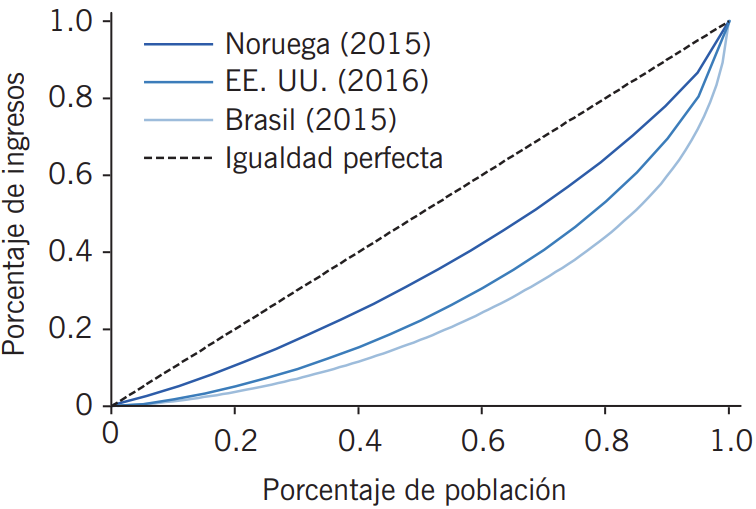
\includegraphics[scale=.35]{codigoFuente/tareas/decisiones/image/gini.png}
	\end{center}
	\vspace{.7cm}
    Si una de las curvas de Lorenz se encuentra debajo de otra, la distribución  es más desigual que la otra. Por lo tanto está claro que en la figura Noruega el más igualitario y Brasil el más desigual de los tres.\\
    El índice de Gini es el área entre la curva de Lorenz y la línea de igualdad perfecta, sobre el área total debajo de dicha linea. Ya que es un índice o coeficiente sus valores se encuentra entre 0 igualdad perfecta y 1 (Sólo una persona obtendría los ingresos de los demás), en consecuencia cuanto menor es el valor de Gini, más igualitaria es una sociedad. 
    Según (https://data.oecd.org/inequality/income-inequality.htm) Noruega tiene un índice de 0,27, donde podemos considerar de baja desigualdad, contrariamente a Brasil(2013) con un 0.5. Cabe mencionar que las economías con valores de Gini superiores a 0,5 se consideran muy desiguales este podría ser el caso de Bolivia,  Colombia o Zambia. \\
    Cabe mencionarse que EEUU(2013-2019) se mantuvo con un indice constante y noruega tuvo una alza de desigualdad desde 2014 para adelante.\\\\ 

    % ---------- 2.
    \item  Para el caso de Noruega el sistema tributario se tiene un taza fija aplicable, y una parte progresiva en función a los ingresos. El tipo fijo del impuesto de la renta es del $22\%$. Además, para aquellos cuya base imponible supere las 184.800 coronas (18.480€) anuales, también se aplicará un tipo progresivo.\\\\
    Con respecto a programas de mantenimiento de los ingresos, las mujeres tienen derecho a una baja por maternidad de 46 semanas (cobrando el $100\%$ del salario) y los hombres disponen de 10 semanas de permiso cobrando el $100\%$ de su salario. Por otro lado Las personas desempleadas tienen derecho a cobrar la prestación por desempleo siempre que hayan cobrado menos de $17.000$ dolares aproximadamente en el año anterior o bien menos de unos 34.000 dolares en los tres últimos años. La cantidad a cobrar como prestación es de cerca del $85\%$ de su salario y su duración es de $500$ días.\\\\

    Y con respecto a subsidios a los servicios públicos, el sistema educativo en todos sus niveles es prácticamente gratuito y obligatorio. El sistema de salud es sólo gratuita para menores de 16 años y para mujeres embarazadas y en periodo de lactancia, luego todos deben pagar una cuota anual de 222 dolares que te da derecho a asistencia gratuita durante el resto del año. Los hospitales públicos son gestionados por cuatro Autoridades Sanitarias Regionales, que son supervisadas por el Ministerio de Sanidad y Servicios Asistenciales.




\end{enumerate}







    %--------------------Análisis de coyuntura económica (economistas)---------------------
    %\chapter{Análisis de coyuntura económica y crecimiento (Economistas)}




    %--------------------Análisis de coyuntura económica (no-economistas)------------------
    %\part{Análisis de coyuntura económica (No economistas)}






    %--------------------Métodos cuantitativos (Estadística)-------------------------------
    %\part{Métodos cuantitativos (Estadística)}

\chapter{Introducción}
\begin{itemize}
    \item La estadística comienza con un objetivo, luego por un estudio estadístico para luego crear conocimiento.
    \item Debemos elegir una población para poder sacar conclusiones.
    \item Se debe tener datos primarios, es decir datos que no existen y datos secundarios que se publican en instituciones publicas o privadas.
\end{itemize}




    %--------------------Métodos cuantitativos (Matemáticas)-------------------------------
    %\input{codigoFuente/matemáticas.tex}


    %%%%%%%%%%%%%%%%%%%%%%%%%%%%%%%%%%%%%%%%%%%%%%%%%%%%%%%%%%%%%%%%%%%%%%%%%%%%%%%%%%%%%%%
    %%%%%%%%%%%%%%%%%%%%%%%%%%%%%%%% TÉCNICA ECONOMETRÍA %%%%%%%%%%%%%%%%%%%%%%%%%%%%%%%%%%
    %%%%%%%%%%%%%%%%%%%%%%%%%%%%%%%%%%%%%%%%%%%%%%%%%%%%%%%%%%%%%%%%%%%%%%%%%%%%%%%%%%%%%%%

    %-------------------- Trabajo 1
    \begin{center}
    \textbf{\Large Análisis del impacto de la tecnología en la tasa de desempleo:\\Colombia 2000-2020}
\end{center}
%linea horizontal
\begin{center}
	\rule{1\textwidth}{0.5pt}
\end{center}
\vspace{1.5cm}


\textbf{\large 1. Introducción}\\

El desempleo, a pesar de su disminución a través de los años, es un fenómeno que ha afectado a la sociedad Colombiana desde el año 2015 (Vallejo - 2020). En este trabajo se analizará el impacto de la tecnología en la tasa de desempleo en Colombia, para lo cual se utilizará la metodología de la regresión de mínimos cuadrados ordinarios (MCO), la cual permite estimar la relación entre las variables independientes y la variable dependiente, en este caso la tasa de desempleo.\\

EL Banco Mundial define el desempleo como $"$la proporción de la población activa que no tiene trabajo, pero que está dispuesta a trabajar y que está buscando trabajo.$"$ A su vez, las TIC's mediante la innovación y la globalización, están cambiando las forma de trabajo. Por lo que, nos planteamos la siguiente pregunta:

\begin{center}
    ¿Cual fue el impacto de la tecnología dentro de la tasa de desempleo en Colombia?
\end{center}

Existen varios debates con respecto al influjo de las TIC's en el desempleo. Pero nos centraremos en dos: Minian y Monroy (2018) mencionan que el cambio tecnológico realza la productividad y la competencia y desplazan al esfuerzo humano en actividades que las máquinas son más eficientes. Sumado al trabajo de la Organización mundial del trabajo (OIT), donde menciona que a las TIC's como principal causante del aumento de desempleo en el mundo.\\\\


\textbf{\large 2. Revisión de la literatura}\\

Según la Cimoli y Porcile (2013) el desarrollo tecnológico genera efectos positivos en el sector económico, pero existen la disyuntiva entre el efecto que genera este proceso tecnológico dentro del índice desempleo. En este sentido, Minian y Martinez (2018) en su investigación resaltan que, el cambio tecnológico aumenta la productividad y la competitividad, redefine los modelos de producción y desplaza al trabajo humano en actividades que las máquinas pueden hacer de manera más eficiente. Por su lado Alderete (2019), descubre que cuanto más tecnológica es la ciudad mayor es la tasa de desempleo, por lo que existe una correlación negativa entre la tasa de desempleo y la tecnología. \\

Pero se diferencia de la investigación presentada por Orji (2016) donde sustenta que los resultados muestran una relación positiva pero insignificante entre las TIC y la tasa de desempleo.  En esta investigación, el coeficiente de las TIC implica que a medida que el uso de las TIC aumenta en el $1\%$ la tasa de desempleo también aumenta en un $0,09\%$.\\

 Por otra parte, distintos autores consideran que el desempleo obedece a otros criterios económicos mas que al nivel tecnológico, determinando que el desempleo y el empleo con relación a la tecnología dependen del horizonte temporal, así mismo, para este estudio los cambios en el nivel de desempleo no dependen de las inversiones que se hagan en I+D ni mucho menos en la participación creciente del cambio tecnológico. (García, 2013). 

con los expuestos por Aguilera y Ramos (2016) los cuales muestran que los países con altos niveles de PIB per cápita en la región aun se encuentran en una etapa de desarrollo en la que las inversiones en Gasto Interno en ciencia y Tecnología afectan positivamente al empleo, logrando ganancias de productividad, así mismo dado los resultados, se puede afirmar que promover el desarrollo de las innovaciones podría generar impactos significativos en la creación de empleo, lo cual reduce la tasa de desempleo.

¿Afectan las innovaciones tecnológicas al desempleo?, es una de los cuestionamientos que se
realizan muchos autores y que, Matuzeviciute y Buktus (2017) a través de las estimaciones,
excepto una, no sugieren que las innovaciones tecnológicas (aproximadas por familias de patentes triádicas (tfp) tiene un efecto sobre el desempleo. La tercera estimación muestra una correlación negativa, es decir, una mayor actividad de innovación se asocia con una menor tasa
de desempleo. Casi todas las variables de control incluidas en el modelo son estadísticamente
significativas: IED entrante negativamente y IED saliente asociada positivamente con la tasa
de desempleo, el crecimiento económico y un índice de precios más alto, como consecuencia
del crecimiento económico, se correlacionan negativamente con la tasa de desempleo, un gasto
público más generoso sobre el desempleo parece tener un resultado negativo: aumenta el desempleo debido a la reducción de los costos alternativos del trabajo.

Patiño (2014) y Saez (2012) llegan a la conclusión de que existe una relación negativa entre el
progreso tecnológico y el desempleo solo se podría explicar por el dominio del efecto de capitalización, donde menores tasas de crecimiento de la PTF habrían desmotivado la creación de
puestos de trabajo y generado un aumento en el desempleo. Sin embargo, se encontró que, aun
en el caso extremo en que todo el progreso tecnológico hubiera operado bajo este efecto, la desaceleración de la PTF observada durante el periodo 1996-2000 no logra explicar los incrementos en el desempleo, lo que indica que son otros factores, diferentes al progreso tecnológico, los
que explican este fenómeno.

Finalmente, Saka y Othan (2019) en base a los
resultados se obtiene un coeficiente positivo del gasto en I+D que oscila entre 0.012 y 0.034, lo
que significa que la tecnología aumenta el desempleo general. Estos hallazgos también conducen a la importante inferencia de que, en las economías desarrolladas, el progreso tecnológico
hace que la creación de empleo se vea superada por la destrucción de empleo y el mecanismo de
compensación no es eficaz. En general se puede deducir de estudio que, a medida que aumentan
los gastos en I + D, aumenta el empleo de los trabajadores altamente calificados, mientras que
lo contrario es cierto para los trabajadores poco calificados en las economías avanzadas.
\\\\

\textbf{\large 3. Aplicación empírica}\\

\textbf{3.1. Datos}\\

Los datos que se usaran fueron extraídos del Banco Mundial en los periodos anuales 2000 al 2020.

\begin{itemize}
    \item Variable dependiente:
	\begin{center}
	    \begin{tabular}{rcl}
		Y&=& desempleo total ($\%$ de la población activa total).\\ 
	    \end{tabular}
	\end{center}

    \item Variables independientes:
	\begin{center}
	    \begin{tabular}{ccl}
		TIC &=& Importaciones de bienes de tecnologías de la información y\\
			      &&la comunicación (TIC) ($\%$ del total de importaciones de bienes).\\\\
		I &=& Inversión extranjera directa, entrada neta de capital ($\%$ del PIB).\\\\
		IN &=& Logaritmo de la industria, valor agregado ($ \$ $ a precios actuales).\\\\
		FBC &=& Logaritmo de la formación bruta de capital ($ \$ $ a precios actuales).
	    \end{tabular}
	\end{center}
\end{itemize}
\vspace{.5cm}


\textbf{3.2. Metodología}\\

Realizaremos un análisis univariante de la variable dependiente, desempleo total, para definir un modeo ARIMA adecuado mediante su respectivo correlograma y la expresión final del modelo seleccionado.\\

Luego, se modelizará de manera multivariante por MCO la relación entre las variables independientes y la variable dependiente, para determinar la relación entre ellas.\\

Por último, veremos si existe una relación de cointegración entre las variables y en caso de ser así, llevaremos acabo la estimación del modelo de largo plazo.


\begin{table}[!htbp] \centering 
  \caption{Estadísticos descriptivos básicos} 
  \label{} 
\begin{tabular}{@{\extracolsep{5pt}}lcccccc} 
\\[-1.8ex]\hline 
\hline \\[-1.8ex] 
Statistic & \multicolumn{1}{c}{N} & \multicolumn{1}{c}{Mean} & \multicolumn{1}{c}{St. Dev.} & \multicolumn{1}{c}{Min} & \multicolumn{1}{c}{Median} & \multicolumn{1}{c}{Max} \\ 
\hline \\[-1.8ex] 
Y & 21 & 11.371 & 2.961 & 8.300 & 10.490 & 20.520 \\ 
TIC & 21 & 10.006 & 1.071 & 8.500 & 9.902 & 13.037 \\ 
I & 21 & 3.709 & 1.196 & 1.818 & 4.055 & 7.029 \\ 
lnIN & 21 & 24.874 & 0.531 & 24.009 & 25.078 & 25.553 \\ 
lnFBC & 21 & 24.539 & 0.610 & 23.423 & 24.774 & 25.239 \\ 
\hline \\[-1.8ex] 
\end{tabular} 
\end{table}

Notemos que en todas las variables a estudiar, la media y la mediana tienen datos próximos entre si, por lo que los datos no son atípicos.

\begin{table}[!htbp] \centering 
  \caption{Gráficos temporales} 
  \label{} 
\begin{multicols}{2}
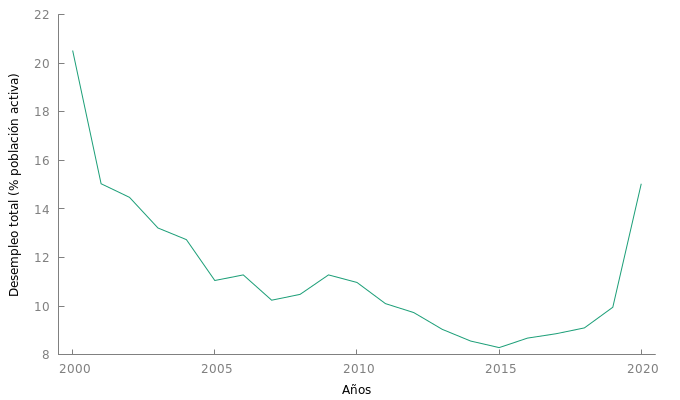
\includegraphics[scale=.33]{r/econometria2/image/desempleo.png}\\
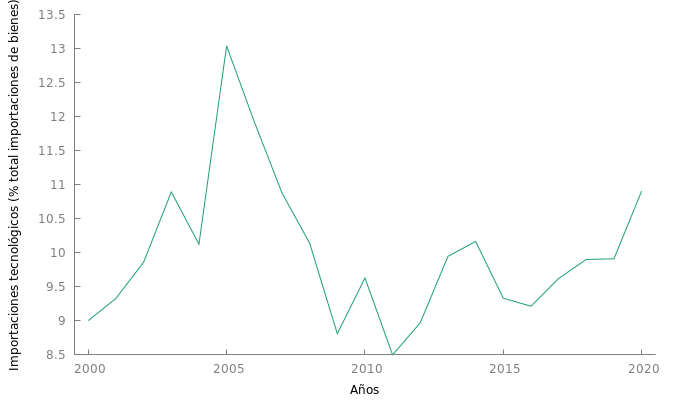
\includegraphics[scale=.33]{r/econometria2/image/TIC.png}\\
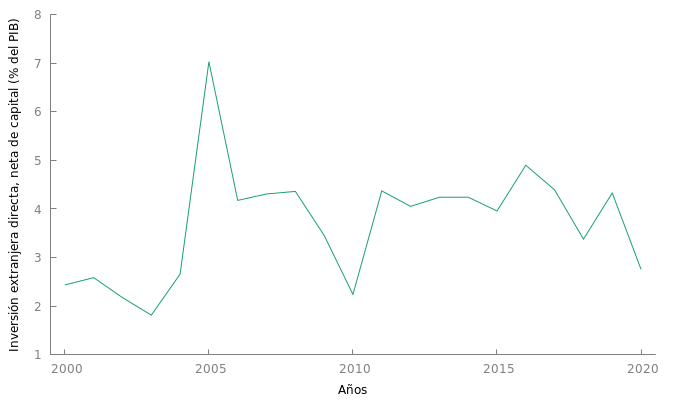
\includegraphics[scale=.33]{r/econometria2/image/I.png}\\
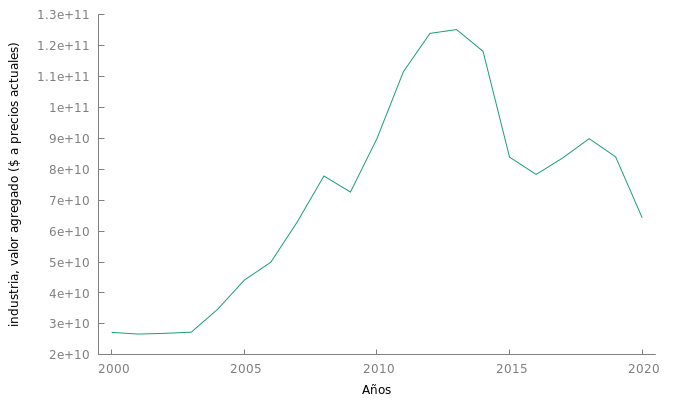
\includegraphics[scale=.33]{r/econometria2/image/IN.png}\\
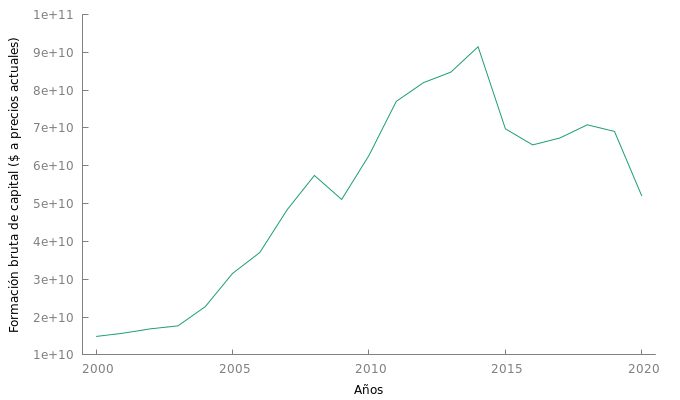
\includegraphics[scale=.33]{r/econometria2/image/fbc.png}\\
\end{multicols}
\end{table}


\textbf{3.2.1. Univariante}\\

Realizamos primero el test de Dickey Fuller donde aceptamos la hipótesis nula de que la serie es no estacionaria, por lo que se procede a realizar la transformación a logaritmos, de donde ya podemos rechazar la hipótesis nula a un $5\%$. Luego elegimos un modelo ARIMA(1,2,1), donde 

\textbf{3.2.2. Multivariante}\\

Modelización MCO de la relación entre las variables. 

\textbf{4. Conclusiones}\\

\textbf{5. Bibliografía}\\
\begin{itemize}
    \item Álvarez, N., y Aldarete, M. V. (2019). Ciudades innovadoras: el efecto sobre el desempleo en la región de Latinoamérica. Trilogía Ciencia Tecnología Sociedad, 193-222.
    \item Banco Mundial. (2013, Septiembre 10). Conectarse para trabajar: Cómo las TIC amplían las oportunidades de empleo en todo el mundo.
    \item Cueva, J. Vivanco, F. Yunga, C. Tapia. Impact of Technology on the unemployment rate: Analysis for Latin American countries in the period 2000 – 2018. \url{http://dx.doi.org/10.54753/suracademia.v9i18.1399}
    \item L. E. Vallejo Zamudio. Repercusiones del desempleo en la estructura productiva colombiana \url{https://doi.org/10.19053/01203053.v39.n70.2020.12035}
    \item M. Cimili y G. Porcile. Tecnología, heterogeneidad y crecimiento: una caja de herramientas estructuralistas. \url{http://hdl.handle.net/11362/4592}
    \item Minian, I., y Martinez, A. (2018). El impacto de las nuevas tecnologías en el empleo de México. Revista Problemas del desarrollo, 1-20.  \url{http://dx.doi.org/10.22201/iiec.20078951e.2018.195.64001}
    \item Techcetera. (2012, Noviembre 27). La tecnología como causante del desempleo: un enorme reto para la humanidad. Retrieved from Techcetera: \url{https://techcetera.co/la-tecnologia-como-causante-de-desempleo-un-enorme-reto-para-la-humanidad/}
\end{itemize}


\textbf{6. Anexos}\\

\begin{center}
Modelo: ARIMA, usando las observaciones 2002--2020 ($T$ = 19)\\
Variable dependiente: $(1-L)^2$Y\\
Desviaciones típicas basadas en el Hessiano

\vspace{1em}

\begin{tabular}{lr@{.}lr@{.}lr@{.}lr@{.}l}
  &
 \multicolumn{2}{c}{Coeficiente} &
  \multicolumn{2}{c}{Desv.\ Típica} &
   \multicolumn{2}{c}{$z$} &
    \multicolumn{2}{c}{valor p} \\[1ex]
const &
  0&487815 &
    0&295962 &
      1&648 &
        0&0993 \\
$\phi_{1}$ &
  $-$0&947063 &
    0&111223 &
      $-$8&515 &
        0&0000 \\
$\theta_{1}$ &
  0&711938 &
    0&338656 &
      2&102 &
        0&0355 \\
\end{tabular}

\vspace{1ex}
\begin{tabular}{lrlr}
Media de la vble. dep. &  0.555789 & D.T. de la vble. dep. &  1.646937 \\
Media de innovaciones &  0.037723 & D.T. innovaciones &  1.437607 \\
$R^2$ &  0.443565 & $R^2$ corregido &  0.410834 \\
Log-verosimilitud & $-$34.22447 & Criterio de Akaike &  76.44895 \\
Criterio de Schwarz &  80.22670 & Hannan--Quinn &  77.08829 \\
\end{tabular}


\vspace{1em}

\begin{tabular}{llrrrrr}
& & & Real & Imaginaria & Módulo & Frecuencia \\ \hline
AR \\ 
& Raíz & 1 & $-1.0559$ & $0.0000$ & $1.0559$ & $0.5000$ \\ 
MA \\ 
& Raíz & 1 & $-1.4046$ & $0.0000$ & $1.4046$ & $0.5000$ \\ \hline
\end{tabular}

\end{center}


    
    %--------------------Técnicas econometricas--------------------------------------------
    %\input{codigoFuente/econometría.tex}

    %%%%%%%%%%%%%%%%%%%%%%%%%%%%%%%%%%%%%%%%%%%%%%%%%%%%%%%%%%%%%%%%%%%%%%%%%%%%%%%%%%%%%%%
    %-------------------- Técnicas de Investigación----------------------------------------
    %%%%%%%%%%%%%%%%%%%%%%%%%%%%%%%%%%%%%%%%%%%%%%%%%%%%%%%%%%%%%%%%%%%%%%%%%%%%%%%%%%%%%%%

	%----------tareas
	%\chapter*{El reto de construir un contrato social progresista y sostenible}

\begin{multicols}{2}

\subsection*{Introducción}

Una de las implicaciones de la primera guerra mundial es la desigualdad. Charles Dickens en su novela $"$historia de dos ciudades$"$, hace mención a la preocupación por la desigualdad en si, no sólo par medirlo si no para estudiar los efectos y consecuencias que lo acarrean.
\begin{center} $"$Era el mejor de los mundos, era el peor de los mundos$"$ \end{center}
Yo me pregunto, realmente acabará en algún momento la desigualdad o por lo menos tendrá una reducción significativa?. A continuación veamos un instrumento que puede ser de utilizar para tal efecto.

\subsection*{Problema}

\begin{center}¿Que es lo que una democracia pluralísta con una economía de mercado sea sostenible, que funcione armoniosamente y prevenga la barbarie política de los años 30?, ¿cuales son las causas del actual y del populísmo?\end{center}

Si se tuviese una respuesta para esta pregunta, seriamos muy útiles de sugerir normas inherentes al progreso social, económico y politico. \\
Una democracia liberal y democrático, puede conciliar progreso social y democracia siempre que haya un contrato social, no un pacto, que retóricamente tiene que ser un compromiso entre aquellos a los que le va bien con el sistema de democracia liberal y aquellos que tiene el riesgo con el disfrute de quedarse atrás en la falta de ingresos y oportunidades. Este compromiso debe ser apoyado por instituciones, de donde la igualdad de oportunidades no se puede garantizar sin una buena educación. \\\\
Parte del contrato social de la izquierda de la época en los años $50's$, se basó en acuerdos de legitimización de mercados capitalistas, y por lo tanto estos años fueron gratificantes. \\
Menciona John Rwals, que los científicos y filósofos morales y politicos se preocupan por conocer y aplicar contratos sociales, todo lo contrario a los economistas; esto, tal vez, por hecho de que se cree que los mercados libres funciona armoniosamente, que por desgracia tuvo un gran éxito.\\
De todas formas y gracias a algunos indicadores se menciona que la productividad esta decreciendo por causas del contrato social. De lo que se puede inferir que el crecimiento vendrá siempre y cuando se tenga un detallado e inteligente contrato social. En la percepción de Antón, será un crecimiento dual.\\\\
Algo curioso que pasa estos últimos años es que la pandemia reciente esta trayendo una rehabilitación del mencionado contrato social. Y no así la crisis del $2008$ donde el contrato social se destruye con recortes y política fiscal contractiva contrario a lo que se ve ahora con políticas expansivas y dirigida a la educación.\\\\
Así y no menor es el hecho de que no debemos fijarlos en la prosperidad perdida, si no al miedo de perdidas futuras en temas de prosperidad siempre tratando de evitar el malestar socio-económico que desencadenaría en la segunda derivada de manifestaciones culturales.\\\\
A continuación se toca algunos puntos importantes referentes al problema.

\subsubsection*{La sostenibilidad social y democracia}
Keynes menciona que son las ideas y no los intereses son lo que al final marcan el rumbo de la sociedad,  por lo tanto debemos estar consientes de que algunas ideas de Adam Smith son fundamentales en la modelización óptima en la sociedad, más concretamente, la idea de sostenibilidad en el siglo $21$ moldeará la economía durante décadas. Por ejemplo la sostenibilidad medioambiental ya es parte del ser humano en si, pero aún no somos responsables de aquello y de lo que implica y el impacto positivo de tenerun contrato social democrático.\\
Si no somos capaces de garantizar el pleno empleo, es decir la sostenibilidad social, entonces se arriesga los temas inherentes al medio ambiente y  democracia. Debemos tomar en cuenta que todos los efectos que estimamos funcionará a través de la capacidad que tengan las democracias. La democracia es como un árbol que hecha raíces donde la raíces son la estabilidad social.

\subsubsection*{Laberintos de la prosperidad}
Cuando una sociedad percibe que no tiene oportunidades, entonces se debe reducir la desigualdad. Pero como reducir la desigualdad? Cuales son las fuentes de la desigualdad?.\\
Esto podría ser por el mal funcionamiento de la redistribución que tiene lugar desde los años $30$ y/o de la poca capacidad de las personas que están en el mercado laboral.\\\\
Una tesis relacionada está en la mesa, las fuentes mas importantes de la desigualdad son el desempleo y los salarios.  Como buscamos la prosperidad.? (Se indica un cuadro con un laberinto que nos podría llevar a esa
prosperidad deseada) Se propone una taxonomía para poder tener políticas económicas más útiles.

\subsubsection*{Una nueva epifanía económica}
Mencionemos un dilema, la ley de Ockham, que entre la busque de la eficiencia y la equidad el autor se
preocupado por la desigualdad. Pero con el único detalle de que al querer relacionarlo obtiene una función negativa, que es contrario a lo que se sabe hoy en día. A ésto se tiene una mejora razonable de la justicia social que no perjudica al estado; es más sana y sostenible en el tiempo, como una epifanía. Por lo tanto se necesita apóstoles para traer una economía más sostenible.

\subsection*{Conclusiones}
En toda medida política y económica se tienen ganadores y perdedores que se debe identificar, de todas maneras es casi un hecho que debemos investigar este tiempo en ese sentido, donde combinemos objetivos deseables para la sociedad y propongamos soluciones que la sociedad compre, en otras palabras los economistas tenemos que dirigirnos no solo a los políticos si no también a la sociedad en si. \\
Creemos en una democracia pluralista, donde  aprendamos a vivir en sociedad.

\end{multicols}


	%---------- Akerlof-1970
	%\begin{center}
    \large
    \textbf{EL MERCADO DE LIMONES :\\
    LA INCERTIDUMBRE DE LA CALIDAD Y EL \\
    MECANISMO DEL MERCADO}\\
    \vspace{.5cm}
    \normalsize
    \textbf{George A. Akerlof}
\end{center}

\vspace{2cm}

\begin{enumerate}[\bfseries 1.]

    %1.
    \item \textbf{Qué te ha llamado más la atención del contenido de este post?.}\\\\

	Me llamaron la atención dos puntos. El primero: Como una teoría macroeconómica. Es decir, la teoría del crecimiento y su aplicación a la educación, podrían llevar a Akerlof a escribir sobre un tema microeconómico, para luego ganar el premio Nobel. Trato de decir que podemos iniciar una investigación económica de varias perspectivas. \\
	 Akerlof estaba claro de cada argumento que escribió. Por lo que el segundo punto que me llamo la atención, es la constancia y perseverancia que tuvo para que alguna revista pueda publicar su hallazgo. \\\\

    %2.
    \item \textbf{Lee el artículo “The Market for Lemons” (QJE, 1970) y resume, con tus propias palabras las siguientes partes: la tesis (pregunta), métodos (el cómo testar la pregunta empírica o resolverla) y los resultados más relevantes.}

\end{enumerate}



    %--------------------Globalización económica y desarrollo social------------------------

	%----------tarea 1
	%


\section{Informe de situación 2015}

    \subsection{Indicadores generales}
    En 2015 la economía Boliviana alcanzó un producto interior bruto de 33.000 millones de dólares y una población de 10.725 millones. Bolivia representaba el 0,04 \% del PIB mundial y el 0,15 \%  de la población. De donde se tiene que el peso relativo de Bolivia en términos de PIB es de 0,27 veces el valor relativo de la población.\\
    El PIB per cápita fue de \$ 3.077,03, valor inferior al promedio mundial (0.3 veces menor), aunque 53.58 \% por encima del valor promedio de los países de ingreso medio bajos. En términos dólares por persona / día, un Boliviano disfruta de una cantidad diaria de bienes y servicios equivalente a 8.43 dólares al día, significativamente inferior a los 27,87 dólares correspondientes a la media mundial.\\
    En el caso de la economía Boliviana, prestamos especial atención a la tasa de paro y a la tasa de inflación. Por lo que en 2015 se registró una tasa de desempleo solo del 3.07 \%, inferior al promedio mundial (5.45\%). En cuanto a la inflación, los precios en Bolivia disminuyeron en 4.62 \%, La trayectoria descendente de la inflación estuvo determinada principalmente por el buen desempeño del sector agropecuario, bajas presiones inflacionarias externas y la estabilidad cambiaria, así como por el comportamiento estable de las tarifas de servicios y las expectativa inflacionarias moderadas \footnote{https://www.reuters.com/article/economia-bolivia-inflacion-idLTAKBN0UL12D20160107}, siendo una de las más bajas de América del Sur. \\

    \subsection{Oferta: Crecimiento}
    La economía Boliviana hacia 2015 creció un 4.86 \%, superando en casi dos veces a los países de referencia, que crecieron de media a un ritmo del 2.86 \%. A pesar de un significante crecimiento el PIB per capita se mantuvo igual en relación al año anterior.\\
    Suponiendo que el factor trabajo es homogéneo, y que se emplea la misma tecnología y una dotación fija de los restantes factores productivos Bolivia tuvo una productividad aparente total superior a los países de ingreso medios bajos, pero extremadamente inferior al promedio mundial, es decir, cada persona empleada tendría que haber recibido 4735 dolares al año muy por debajo de los 17318 dolares de la media mundial.\\
    Las diferencias de renta per cápita y de productividad se reducen cuando expresamos las unidades en paridad de poder adquisitivo. En Bolivia un consumidor puede adquirir una cesta de bienes y servicios más abundante. Con respecto a la Latino América, tenemos una productividad media inferior de 14877 dólares per cápita frente a 32444 dólares.


    \subsection{Oferta: Especialización productiva y eficiencia}
    En términos de producción y empleo sectorial, la economía Boliviana mantiene las características de un país en vías de desarrollo, ya que se tiene un bajo peso de la agricultura en términos de producción y empleo (más del 5 por ciento), peso decreciente de la industria pero cerca del 25 por ciento de referencia y mayor importancia absoluta en relación con el sector servicios (menos del 70 por ciento). Por lo que Bolivia encaja de manera casi ideal a este perfil.\\
    No está por demás señalar que la agricultura generó 337905 millones de dólares que equivale al 0.12 \% del promedio mundial. La industria genero 831685 millones de dolares y los servicios generaron 1517230 millones de dolares el cual equivale al 0.04\% y 0.03 \% respectivamente al promedio mundial.\\
    Lo dicho anteriormente va acompañada de una baja productividad en todos los sectores. Ya la comparación de los valores de Bolivia con respecto al mundo ya es muy ilustrativa, como veremos a continuación: Frente a una productividad agrícola en Bolivia de 1741 dólares, la media mundial es de 2.278 dólares. Frente a una productividad  de la industria de 5297 dolares, la media mundial es de 19700 dolares y frente a una productividad de servicios de 4387, la media mundial es de 22371 dolares. Está claro que nuestras metas de crecimiento deben basarse en el crecimiento de la productividad en todos los sectores en especial en de la industria y servicios.\\


    \subsection{Oferta: Especialización comercial y competitividad}
    El sector exterior es el mejor barómetro para medir la competitividad de un país. En el mercado interno, el gobierno goza de cierta autonomía para establecer reglas que protejan a sus empresas de empresas extranjeras. Esta opción no encaja en los mercados extranjeros.\\
    En 2015, la economía española mostró una tasa de apertura del 63,6 por ciento. Este peso del sector exterior sobre el PIB español es un valor muy cercano a las medias mundiales, las rentas altas y la Unión Europea. Podemos decir que el grado de integración de España en comercio exterior es alto. Ese año, como lo muestra la tasa de cobertura, se registró un superávit comercial, por lo que los ingresos por exportaciones cubrieron más que suficientemente los pagos requeridos por las importaciones. Los ingresos de exportación superaron a las importaciones en un 7,4 por ciento. Este superávit representó el 2,2 por ciento del PIB.\\
    El volumen de las exportaciones españolas de bienes (sin incluir los ingresos por servicios) supuso el 1,60 por ciento de las exportaciones mundiales, lo que está en consonancia con el peso de la economía española en el PIB mundial, como vimos antes, del 1,70 por ciento. Gran parte de estas exportaciones de mercancías son manufacturas (71,98 por ciento), cifra muy cercana a los grupos de referencia. Destaca el elevado peso de las exportaciones de alimentos (16,25 por ciento), más de siete puntos porcentuales por encima de los grupos de referencia. La importancia económica de la agricultura española se pone de manifiesto de nuevo.\\
    Dentro de las exportaciones de manufacturas, los productos de alta tecnología representaron el 7,15 por ciento de las exportaciones de mercancías. También encontramos aquí una cifra sensiblemente inferior a los grupos de referencia: más de diez puntos porcentuales respecto a los países de renta alta y la Unión Europea7. Dada la especial relevancia de este tipo de productos sobre las posibilidades de crecimiento futuro, podemos señalarlo como otro ámbito en el que los sectores económicos españoles necesitan mejorar.\\

    \subsection{Demanda: Sostenibilidad}
    Desde el punto de vista de la demanda agregada podemos analizar si la estructura de gasto de un país es sostenible en el tiempo. El principal objetivo de la actividad económica es satisfacer las necesidades actuales de las personas, por lo que es evidente que gran parte de la la producción es demanda para el consumo, ya sea privado o público. Vemos que los porcentajes de consumo privado y consumo español son muy similares a los grupos de referencia. Casi el sesenta por ciento del PIB se destina al consumo privado y el veinte por ciento al consumo público.\\
    El consumo futuro dependerá del esfuerzo que se haga en términos de inversión y de cómo se financie esta inversión. Para ello es importante conocer la capacidad de ahorro del país. Un país se puede salvar con recursos internos y también con recursos externos. Aquí es fundamental conocer la relación entre tasa de inversión, tasa de ahorro y balanza comercial.\\
    En 2015, España tenía una tasa de inversión del 20,4 por ciento, cifra inferior a la tasa de ahorro, que fue del 22,7 por ciento. Esto significa que parte del ahorro interno ha sido más que suficiente para financiar necesidades de financiamiento y lograr cierta capacidad de financiamiento de otras economías. Este ahorro externo se da gracias a que las entradas de divisas generadas por las exportaciones superaron los pagos que hubo que afrontar para realizar las importaciones. El superávit comercial representó el 2,3 por ciento.\\
    Respecto a estos indicadores, no existen puntos de referencia que permitan evaluar de forma inmediata si un país se encuentra en una situación de equilibrio económico y financiero. En teoría, los países con superávit comercial están en mejores condiciones para afrontar el futuro, porque están generando ahorro, condición básica para poder invertir y crecer económicamente. Pero también es una condición necesaria para el crecimiento económico que un país adquiera deuda externa para cubrir las carencias del bajo ahorro interno. Es la forma de poder renovar el aparato productivo para ser más eficientes y competitivos en el futuro. Sin embargo, el país debe incrementar sus ahorros con el tiempo, incrementar sus exportaciones y así convertirse en acreedor neto. Este diagnóstico sólo lo podemos hacer a través del análisis de la evolución del país en un período más largo y acompañado de otros indicadores que nos muestren dónde se están utilizando los ahorros o los préstamos.\\
    Ciertos indicadores son especialmente útiles para esta evaluación, como el número de investigadores a tiempo completo, el gasto en I+D, las emisiones de CO2 y el consumo per cápita per cápita. Estos cuatro indicadores recogen decisiones tomadas en el presente que tendrán un especial impacto en el futuro. Dedicar recursos a la investigación oa reducir el impacto de la actividad económica sobre el medio ambiente no tiene hoy repercusiones inmediatas, pero sus efectos acumulativos en el tiempo pueden tener un impacto significativo en el crecimiento futuro del país. Es probable que cuantos más investigadores contratemos, más gastemos en investigación y desarrollo, menos contaminemos y menos energía usemos hoy, más probable es que siga creciendo de forma sostenible en el futuro.\\
    Para el año 2015, los indicadores de investigación mostraban un déficit en España respecto a los grupos de referencia. Tanto el número de investigadores como el gasto en I+D están por debajo de la media: 2655 investigadores por millón de habitantes frente a una media de 4014 países de ingresos altos9. El gasto español en I+D alcanzó un valor del 1,22 por ciento del PIB cuando la media es del 2,5 por ciento en los países de renta alta y del 2,05 por ciento en la Unión Europea. La brecha es grande ya que los valores más altos rondan el 3 por ciento.\\
    Para las emisiones de CO2 y el consumo de energía no tenemos los valores para el año 2015, pero podemos usar los valores más recientes para el período 2010-2015. Ahí podemos ver que España ha mantenido un perfil positivo, con valores por debajo de la media en ambos casos. Sobre todo, destaca que los valores no están por debajo de los promedios de los países de altos ingresos. Frente a valores de 10,98 Tm per cápita y 2.571 Kg equivalentes de petróleo en este grupo de países, los españoles emitieron 5,03 Tm per cápita de CO2 y consumieron 2.571 Tm equivalentes de petróleo por persona.

    \subsection{Demanda e ingreso: Capital}
    La acción del sector público y la distribución del ingreso permiten abordar la cuestión de cómo la actividad económica afecta otras variables sociales, especialmente la equidad entre las personas. El sector público tiene la capacidad a través del gasto público de cambiar la distribución del ingreso que se produce en el mercado. El gasto público en educación y el gasto público en salud juegan aquí un papel relevante. Si hay elementos se utilizan para este fin, el resultado se observará en los indicadores de distribución del ingreso.\\
    A medida que desagregamos los componentes del PIB, será más difícil encontrar información actualizada para todos los países. El número de países que presentan todos los datos ya es menor, falta homogeneidad temporal en muchos indicadores, por lo que los promedios por grupo ya no son representativos. En este caso, conviene tomar como referencia ciertos países que sirven como casos modelo. Así, Suecia tiende a ser un país de disparidades reducidas en la distribución del ingreso; Estados Unidos es un país de altos ingresos con grandes disparidades de ingresos; y Francia está en una situación intermedia.\\
    En primer lugar, destacamos que España ha realizado un menor esfuerzo relativo en cuanto a recursos destinados a educación y sanidad respecto a su PIB: un 6,5 por ciento en sanidad y un 4,3 por ciento en educación. Tanto Estados Unidos11 como Francia mantienen valores más altos, con Suecia con un 9,2  \% en salud y un 7,7 \% en educación.\\
    En segundo lugar, España en términos de índice de Gini muestra un valor de 36,20, más cercano a la situación de Estados Unidos (41,00) y muy por encima de Suecia (29,20). El veinte por ciento de la población española con mayor renta per cápita (quintil superior) concentra el 42,1 por ciento de la renta, mientras que el quintil inferior recibe sólo el 5,8 por ciento. Frente a un ingreso promedio de $ 54.227 de los más ricos, los más pobres recibieron $ 7.479. En términos relativos, la tasa de desigualdad en España fue de 7,26 ese año. Esta ratio de desigualdad es menor en Suecia (4,59) y Francia (5,18). Vemos que en Estados Unidos la renta media del grupo más rico era 9,10 veces superior a la renta media del grupo de población más pobre. España se encuentra en una situación intermedia respecto a estas referencias.
    
    \subsection{Resumen}
    Con los datos del año 2015 podemos deducir que España muestra características de País Desarrollado. Su ingreso per cápita está claramente dentro del grupo de países de altos ingresos. Mantiene una estructura productiva y comercial desarrollada de países, así como una equidad económica más cercana a este grupo de países. También notamos que tiene ciertas debilidades o aspectos a mejorar, como la baja utilización de mano de obra y la necesidad de dirigir la inversión a actividades con mayor potencial de crecimiento futuro. Determinar en qué medida estas características apuntan a un crecimiento equilibrado y sostenible requiere una evaluación de un período más amplio. Este es el objetivo de la segunda parte del informe.

\section{Informe de evolución 1990-2015}
A partir de los gráficos del documento Indicadores.xlsx evaluaremos la economía española en el periodo 1990-2015. Como hemos dicho, se trata de determinar si la economía española crecerá económicamente durante ese período de forma equilibrada y sostenible.

    \subsection{Crecimiento}
    En el gráfico 1.1 podemos ver cómo ha evolucionado la dimensión relativa de España desde el punto de vista económico. En términos de población, España está perdiendo peso sobre el conjunto mundial. A principios de los 90 la población española suponía cerca del 0,73 por ciento de la población mundial, y hoy ya es el 0,63 por ciento. La tendencia de pérdida de peso, aunque lenta, es claramente negativa.\\
    La tendencia demográfica estuvo acompañada de una tendencia cíclica desde el punto de vista del peso del PIB. El período 1992-2000 experimentó una pérdida de peso relativa. Ha pasado del 2,37 por ciento del PIB mundial al 1,60 por ciento. La cifra inicial se recuperó durante los años 2000-2008, pero volvió a perder peso económico de 2008 a 2016. Más estable fue la evolución de las exportaciones, que se movieron entre un valor mínimo de 1,79 por ciento en 1993 a un valor máximo de 2,29 en 2003. Recientemente, es 1.80 por ciento.\\
    Es interesante notar cierta correlación entre el PIB y las exportaciones. Cuando el peso relativo de las exportaciones es superior al peso relativo del PIB (período 1992-2003), en los años siguientes aumenta el peso relativo del PIB (período 2000-2008). Y viceversa: un peso relativo de las exportaciones inferior al peso relativo del PIB (período 2008-13) provoca una posterior pérdida de capacidad económica relativa de la economía española (2012-16). De mantenerse esta asociación, esperamos un aumento del peso relativo de España en los próximos años. Este resultado no debe sorprendernos: el aumento de las exportaciones implica que estemos en ingresos externos para incentivar una mayor producción interna.\\
    La caída relativa del PIB no significó la ausencia de crecimiento del PIB per cápita. El Gráfico 1.2 muestra que el PIB per cápita de los españoles creció durante este periodo. Si estaba por debajo de los \$ 25.000 constantes a principios de la década de 1990, estaba aumentando constantemente hasta un máximo de \$ 32.303 por persona en 2008. Prácticamente, el ingreso per cápita se multiplicó por 1,4 entre 1990 y 2008. El gráfico muestra que una brecha constante de ocho mil dólares se mantiene con respecto a los países de ingresos altos, la diferencia relativa se ha reducido en 3,78 puntos (en números índice). Esta tendencia estalló en 2008 como resultado de la recesión económica mundial que comenzó ese año. En el caso de España, afecta con más intensidad y provoca un descenso del PIB per cápita. En 2013 se tiene un PIB per cápita de \$ 30.532, muy similar a los de doce años antes.\\
    Una explicación de esta trayectoria de la economía española se resume en el Gráfico 1.3. Este gráfico muestra cómo ha crecido el PIB per cápita en comparación con la evolución de la productividad y el empleo per cápita, las dos variables que ayudan a identificar qué estrategia de crecimiento sigue un país. Durante este periodo hemos observado que, salvo algunos años, la estrategia de crecimiento de España siempre ha estado claramente basada en aumentar la producción aumentando el empleo. Entre 1995 y 2008, la productividad apenas aumentó 12. El crecimiento del PIB per cápita observado más recientemente sigue basándose en esta estrategia. Por tanto, en términos de crecimiento podemos afirmar que no estamos siguiendo la estrategia más adecuada.\\

    \subsection{Especialización sectorial y productividad}
    La evolución española de la estructura sectorial de la producción muestra una clara tendencia a acercarse al perfil de los países desarrollados. El peso del sector servicios sigue aumentando, tanto en la producción como en el empleo, en ambos casos ya por encima del 70 por ciento del total del sector. El sector industrial empieza a situarse en torno al 20 por ciento, perdiendo peso relativo principalmente en términos de empleo. En el caso de la agricultura, el valor agregado parece mantenerse en torno al valor de 2,5 por ciento, pero el empleo mantiene una tendencia a la baja.\\
    Los cambios anteriores están íntimamente relacionados con la evolución de la productividad. Si bien la agricultura reduce su fuerza de trabajo, el gran aumento de la productividad (duplicada en el período 1994-2016) le permite mantener su contribución a la producción total. En el caso de los servicios, la productividad no experimentó crecimiento durante el período de análisis. Como sabemos, este es un sector que, por su propia naturaleza, muestra dificultades para mejorar su productividad. En la mayoría de las ramas del sector servicios, aumentar la producción requiere aumentar el número de empleados (hostelería, restauración, educación, sanidad, etc.).\\
    Respecto a la industria, la evolución de la productividad muestra un claro cambio de tendencia. Entre 1994 y 2008, la productividad industrial disminuyó levemente. Como decíamos antes, sucedió que fue un periodo en el que España recurrió al aumento del empleo para aumentar la producción, sin que se produjeran en promedio aumentos de productividad. A partir del año 2008 observamos un incremento muy significativo en la productividad. Sin embargo, debemos ser escépticos sobre los fundamentos reales de tal fenómeno. Existen otros factores que pueden estar provocando un aumento ficticio de la productividad, como son: el despido de los trabajadores menos productivos, la reducción de los costes laborales y los efectos de la evolución del tipo de cambio euro-dólar. Durante este período se produce una devaluación del euro que provoca un aumento de la producción calculada en dólares. Se necesita un análisis más profundo de estos factores para concluir con mayor precisión la evolución de la productividad.\\

    \subsection{Comercio exterior y productividad}
    Durante el período 1990-2016 el coeficiente de apertura español mostró una tendencia mayoritariamente creciente. A principios de la década de 1990, el volumen de exportaciones e importaciones representaba menos del 40 por ciento del PIB y, al final del período, la cifra superaba el 60 por ciento. En 2009 se produjo una fuerte caída, de casi diez puntos porcentuales. Aún así, el coeficiente fue del 46,5 por ciento, por encima de los valores iniciales del período.\\
    La evolución de la tasa de cobertura es muy diferente, ya la vez muy ilustrativa de las peculiaridades del sector exterior español. Los ciclos fuertemente deficitarios (tasa de cobertura en torno al 80 por ciento) se combinan con ciclos de balance moderados. Se destacan los más destacados en los últimos años 2012-2016, logrando superávits de 10 puntos porcentuales. Parece que el crecimiento económico español depende en gran medida de las exportaciones, pero una vez que la tasa de variación del PIB es alta, la propensión a importar crece en mayor proporción.\\
    Gran parte de este efecto cíclico está relacionado con la fabricación, ya que suele representar entre el setenta y el ochenta por ciento de los ingresos. Observamos que durante los primeros diez años del período las exportaciones de manufacturas aumentaron su peso relativo, acercándose al ochenta por ciento del total. Sin embargo, desde 2001 se ha iniciado la pérdida relativa de peso, cayendo al 67,79 por ciento en 2012.\\
    ara el crecimiento económico, las exportaciones de bienes de alta tecnología juegan un papel relevante. He aquí un aspecto que debería mejorar la economía española. Su volumen de exportaciones de esta clase está entre el 0,72 por ciento y el 1,26 por ciento de las exportaciones totales de alta tecnología del grupo de países de ingresos altos. Este valor es inferior al peso de la economía española en el PIB total (entre el 2,5 y el 3,5 por ciento) y en las exportaciones totales (entre el 2 y el 3 por ciento) tomando como referencia los países de renta alta.\\

    \subsection{Sustentabilidad}
    La evolución del ahorro y la inversión permite valorar si el modelo de crecimiento de la economía española estuvo acompañado durante este periodo de criterios de sostenibilidad. Podemos observar en el Gráfico 4.1 que durante el periodo de análisis la economía española 12 atravesó etapas de capacidad de financiación externa y etapas de necesidades de financiación, aunque predominaron estas últimas, es decir, los años en los que la tasa de ahorro fue menor que la de inversión. . Básicamente, podemos ver que el crecimiento económico del PIB experimentado en los años 1995-2007 fue financiado en términos netos por financiamiento externo. Con una tasa de financiación equilibrada en 1996-1997, la tasa de inversión creció más rápido que la tasa de ahorro, lo que resultó en una tasa de financiación negativa de casi seis puntos porcentuales en 2006.\\
    Una tasa de financiación negativa no es necesariamente indicativa de una mala estrategia de crecimiento. Es obvio que si un país quiere crecer necesita financiamiento e inversión extranjera que le permita innovar su proceso productivo para ser más competitivo en los mercados externos. La condición para la sostenibilidad financiera es que en los próximos años aumente el PIB, aumenten los ingresos y la economía comience a reducir sus déficits comerciales y pagar los préstamos. En el caso de la economía española podemos decir que durante ese periodo el PIB y la renta aumentaron. Sin embargo, no había indicaciones claras de que se cumplieran otras condiciones. Ya sabemos que hasta 2007 el déficit comercial iba en aumento. Observamos que durante este período el esfuerzo en innovación, promediado por el gasto en I+D sobre el PIB (Gráfico 4.2), fue aumentando del 0,78 por ciento en 1996 al 1,35 por ciento en 2010. Sin embargo, aún existe una brecha importante con respecto al promedio de los países de altos ingresos, que en ese período aumentó de 2,14 por ciento a 2,37 por ciento. Obviamente, gran parte del gasto en I+D no se hará efectivo hasta más adelante, pero la disminución del esfuerzo de investigación entre 2010 y 2014 sugiere que la brecha se ampliará.\\
    Los indicadores seleccionados en el Gráfico 4.3 de sostenibilidad ambiental también muestran que el modelo de crecimiento español fue más contaminante y más consumidor de energía en comparación con los países de renta alta. Durante los años 1990-2007 hubo una clara tendencia a emitir relativamente más toneladas de CO2 al medio ambiente y un mayor consumo de energía per cápita. En ambos se experimentó una variación de casi 20 puntos porcentuales. Pensamos que contaminar y consumir más energía con otros países acaba dificultando competir a largo plazo en tecnologías o patrones de consumo más respetuosos con el medio ambiente.\\

    \subsection{Equidad}
    Podemos afirmar que, en general, durante el período 1990-2016, el consumo público aumentó a un ritmo mayor que el PIB (Gráfico 5.1), representando el primer indicador casi cinco puntos porcentuales más que el segundo. A pesar de la tendencia a la baja de los últimos años, el porcentaje de consumo público se ha mantenido por encima del inicio del período. Este mayor consumo público estuvo acompañado de un aumento tanto del gasto público en educación como en salud. Entre las dos partidas de gasto hay un incremento de un punto porcentual sobre el PIB para el período 2004-2014. Sin embargo, este aumento no tiene efectos similares en la distribución del ingreso (Gráfico 5.2). Todo lo contrario. En el período 2004-2016 hubo aumentos en el índice de Gini, de 31,8 a 36,2, provocando una mayor disparidad de casi cuatro puntos entre el decil superior y el decil inferior.\\
    La falta de información para todo el período nos obliga a estar muy atentos a la evolución del patrimonio. Para una visión más completa sería necesario realizar un análisis paralelo con datos del INE o con datos de Eurostat. Podemos comentar aquí que estas fuentes confirman que la tendencia en los últimos años ha sido hacia una mayor concentración del ingreso, a pesar de la reducción de las desigualdades operada en el período 1995-2004. Es posible que la intervención del Estado no esté contrarrestando esta mayor desigualdad porque todavía existe una brecha de alrededor de cinco puntos porcentuales entre la Unión Europea y España en términos de gasto público sobre PIB.

    \section{Conclusiones}	
    La economía española mantuvo una favorable senda de crecimiento entre el período 1990-2007, especialmente a partir de 1995, pero entró en crisis a partir de 2008. Este crecimiento ha contribuido a que España consolide ciertas características de los países desarrollados, pero también aclare sus debilidades. Este informe muestra que hay una serie de indicadores que parecen más apropiados para evaluar si el proceso de crecimiento del PIB o PIB per cápita ha sido equilibrado y, sobre todo, sostenible en el largo plazo. Estos indicadores incluyen lo siguiente:

    \begin{itemize}
	\item Productividad 
	\item Empleo per cápita 
	\item VEB Agrícola  
	\item Empleo agrícola 
	\item Productividad sectorial 
	\item Exportaciones de bienes y servicios  
	\item Exportaciones de alimentos 
	\item Exportaciones de Manufacturas de Alta Tecnología. 
	\item Tasa de ahorro  
	\item Tasa de inversión  
	\item Inversión en I+D  
	\item Gasto público sobre PIB. 
	\item Índice de Gini o Indicador de Desigualdad
    \end{itemize}

    En algunos de estos indicadores, la economía española ha convergido considerablemente a la media de los países desarrollados desarrollados de referencia. En otros indicadores persisten divergencias que ayudan a comprender las dificultades del modelo de crecimiento económico español para competir eficientemente en el contexto de la globalización sin perder de vista los objetivos sociales. Por ambas razones, la experiencia española puede servir de referencia para otros países más alejados de los niveles de desarrollo económico y social de la mayoría de los países de renta alta que consideramos economías desarrolladas.





	

	%----------tarea 2
	%
\section{Indicadores económicos}

    \subsection{Situación económica reciente}
    Mozambique es un país de 28 millones de habitantes con una renta per cápita de 528,31 dólares en 2015. Está dentro del grupo de países de renta baja, y por debajo de la media. Cabe señalar que en el período 1990-2015 el PIB creció a una tasa de 7,6 por ciento y la población a 3,04 por ciento. Como resultado, el PIB per cápita aumentó a una tasa promedio acumulada de 4,43 por ciento. Ha ganado así un peso relativo a nivel mundial y especialmente dentro del grupo de países de bajos ingresos.\\
    El desglose del PIB per cápita en productividad y empleo per cápita revela que es un país con baja productividad en comparación con los países del grupo de ingresos (80,27 por ciento). Hay una alta utilización del empleo, 59,01 por ciento de la población total, aunque es baja en comparación con su grupo de referencia (68,28 por ciento).\\
    Este es un país con un alto peso del sector primario. Esto representa el 22,94 por ciento de la producción y el 73,56 por ciento del empleo. Llama la atención la desproporción en el sector industrial entre el peso del valor agregado (19,65 por ciento) y el empleo (4,28 por ciento). Parte de esta actividad industrial está relacionada con la explotación de minerales (carbón, sal, bauxita, oro, grafito, piedras preciosas, gas natural y mármol). Gran parte de las exportaciones de productos básicos son minerales (38,46 por ciento) y energía (30,38 por ciento). Dado que es un país costero, el turismo proporciona una gran cantidad de ingresos para los turistas que visitan sus playas de clima tropical en el Océano Índico.\\
    Sectorialmente, destaca también la productividad en el sector industrial. Es 50 puntos más alto con el grupo de bajos ingresos. En cambio, en el sector agropecuario la productividad es 35 puntos superior y en el sector servicios es el promedio de los países de bajos ingresos.\\

    \subsection{Evolución económica}
    Durante el período 1990-95 Mozambique aumentó su peso en términos de población mundial: pasó del 0,25 por ciento al 0,38 por ciento. Aunque el peso es menor en términos de PIB y participación de las exportaciones (menos del 0,03 por ciento), también experimentó una ligera tendencia al alza.\\
    Según datos del Banco Mundial, el aumento del PIB se debió principalmente a un aumento de la productividad. También se ha basado en el crecimiento del empleo per cápita, pero esto se considera una cifra negativa, ya que la mano de obra se utiliza de forma intensiva.\\
    La evolución muestra cómo el sector agrícola ha perdido peso relativo. A principios de la década de 1990, la agricultura representaba más del 30 por ciento del PIB total, cuando hoy roza el veinte por ciento. No hay una tendencia clara entre los otros dos sectores. La pérdida de peso de la agricultura es ostensible en lo que a empleo se refiere. A principios de la década de 1990 se situó en el 85,4 por ciento, casi doce puntos por encima del valor más reciente. Ese empleo se concentra en el sector servicios, que duplicó su peso del 11,7 por ciento en 1990 al 22,2 por ciento en 2015.\\
    En concordancia con lo anterior, en los tres sectores hubo un aumento de la productividad. No hay aumento del empleo en la industria porque es el sector con mayor tasa de crecimiento de la productividad. Aumentó de alrededor de \$ 2,000 a \$ 6,000. También se destacó el aumento de la productividad en el sector servicios, de \$ 2.000 a \$ 3.800. La agricultura ha duplicado su productividad, pero sigue siendo baja (en el período pasó de \$ 200 a \$ 400).

    \subsection{Sustentabilidad}
    Durante el período de estudio, Mozambique estaba abriendo su economía al exterior. En la década de 1990, el coeficiente de apertura estaba entre 40 y 60 puntos. En los últimos diez años los valores han crecido hasta los 120 puntos, por lo que el comercio exterior supera al tamaño de la propia economía. Es una economía más exportadora que importadora. La tasa de cobertura siempre ha estado en valores por debajo de los 60 puntos, y más recientemente en los 40 puntos. Este superávit se debe principalmente a las exportaciones de minerales (entre 40 y 60 por ciento) y energía (entre 15 y 30 por ciento). Las cifras de exportación muestran fuertes fluctuaciones, posiblemente debido a las fluctuaciones de los precios. Hubo una fuerte caída en las exportaciones de alimentos, que en la primera parte del período llegó a más del 70 por ciento. Las exportaciones de productos de alta tecnología son insignificantes.\\
    l crecimiento económico anterior ha estado acompañado de una tasa de inversión siempre por encima del 20 por ciento, y en los últimos años muy alta, casi cercana al 60 por ciento. Sin embargo, sorprende que en este país la tasa de ahorro sea prácticamente nula. Se volvió incluso negativo en -64 por ciento en 1990.\\
    Apenas hay gasto en I+D y las cifras de emisiones de CO2 y consumo energético son bastante bajas. Sin embargo, ha habido un fuerte aumento en el consumo de energía en los últimos años.\\
    El consumo público representó entre el 13 y el 25 por ciento del PIB. En el período se destaca la pérdida de peso relativo del gasto militar y el aumento del gasto en educación. La errática evolución del gasto público puede estar explicando que no haya cambios en la distribución del ingreso. El índice de Gini ronda el valor de 50, de modo que el grupo de población más rico concentra más del 40 por ciento de los ingresos, frente al grupo más pobre que se encuentra por debajo del 2 por ciento.\\
    En resumen, a pesar de seguir siendo una economía de bajos ingresos, Mozambique ha crecido económicamente.

\section{Objetivos del milenio}
En cuanto al objetivo 1, erradicación de la pobreza y el hambre, se observan mejoras. El porcentaje de la población que vive con menos de \$ 1,90 al día se ha reducido del 50 por ciento en 1996 al 30 por ciento en 2014 (Meta 1.1). También hay una reducción significativa en la línea de pobreza nacional (Objetivo 1.2). Es difícil interpretar el Objetivo 1.3 con la participación indicada del ingreso del grupo más pobre en el ingreso total. Tampoco hay una tendencia clara. El porcentaje fluctuó sin una tendencia clara entre el 4 y el 5,4 por ciento. Lo más probable es que hubo una mejora, dado que en cuanto a la Meta 1.8, la existencia de bajo peso al nacer en los niños, la proporción bajó del 26 por ciento al 15 por ciento.\\
En cuanto a la educación, hay una mayor tasa de matrícula en la educación primaria (Objetivo 2.1). De valores iniciales del 40 por ciento, en años más recientes ya se ha acercado a valores del 90 por ciento. La tasa de alumnos que terminan la escuela primaria sigue siendo baja (alrededor del 50\%) (Objetivo 2.2), aunque observa un aumento de la tasa de alfabetización los jueves entre los 15 y los 24 años (Objetivo 2.3).\\
En cuanto a la igualdad de género, la proporción de mujeres en la escuela primaria ha aumentado pero sigue siendo baja (7,3 de cada 10 hombres) (Objetivo 3.1), al igual que la proporción de mujeres en el parlamento (1 de cada 10 hombres) (Objetivo 3.3) ,. No hay información sobre el indicador de mujeres que trabajan fuera del sector agrícola (Objetivo 3.2).\\
El progreso más claro se está logrando en el Objetivo 4 de reducir la mortalidad. Tanto la mortalidad infantil como la de menores de 5 años se han reducido notablemente. La primera de 250 a 75 muertes por cada mil nacimientos (Meta 4.1); y el segundo de 160 a 60 por mil nacimientos (Objetivo 4.2). El aumento de la inmunización contra el sarampión está contribuyendo a esta reducción de la mortalidad (Objetivo 4.3).\\
Hay muy poca información sobre el objetivo 5, mejorar la salud materna. Se destaca la tendencia a la baja de la tasa de mortalidad materna (Objetivo 5.1) y de la tasa de fecundidad adolescente (Objetivo 5.4). La primera tasa se ha reducido de 1.300 muertes por cada 100.000 nacimientos a 500. La segunda, con valores iniciales de más de 180 nacimientos por cada 1.000 mujeres de 15 a 19 años, ha bajado a 140 por mil. Sin embargo, sigue siendo alto. Un gran número de partos (más del 60 por ciento) continúan realizándose sin la atención de un médico por médico especialista (Objetivo 5.2).\\
El objetivo relacionado con la enfermedad (Objetivo 6) muestra una evolución muy dispar, que se combina con la falta de información. En el lado positivo, hay más personas VIH positivas tratadas con medicamentos antirretrovirales (casi el 40 por ciento), con un crecimiento casi exponencial (Meta 6.5). En el lado negativo, no hay estabilidad en la disminución de las tasas de mortalidad por tuberculosis (Objetivo 6.9) o en el número de personas afectadas por la malaria (Objetivo 6.6).\\
Con respecto al medio ambiente (Objetivo 7), los indicadores muestran tendencias positivas y negativas. En el lado positivo, las emisiones de CO2 por unidad de PIB se redujeron de 0,40 a 0,20 kg por dólar de PIB en paridad de poder adquisitivo (Objetivo 7.2) y la población con acceso a saneamiento aumentó de 35 por ciento a 51 por ciento (Objetivo 7.8). Sin embargo, la proporción de la población que vive en barrios marginales ha aumentado del 77 al 80 por ciento.\\
Finalmente, con respecto a la meta, 8 Mozambique es un país que recibe casi \$ 100 per cápita en Ayuda Oficial al Desarrollo (Objetivo 8.5). El servicio de la deuda externa cayó del 35 \% en 1995 al 10 \% en 2015, alcanzando el 5 \% durante varios años (Objetivo 8.12). En cuanto a las comunicaciones, se ha incrementado significativamente el número de teléfonos móviles (el 60 \% de la población tiene teléfono móvil) (Meta 8.15), aunque la población con acceso a internet se ha reducido al 15\% (Meta 8.16). Apenas ha habido mejoras en la disponibilidad de telefonía fija, que no llega al uno por ciento de toda la población.\\

\section{Objetivos de desarrollo sostenible}

\section{Resumen}
El crecimiento económico observado por Mozambique durante el período que se examina estuvo acompañado de cambios positivos en algunos indicadores del milenio, pero no en todos. En resumen, pareció tener más efectos sobre la mayoría de las variables relacionadas con la salud. También se observan mejoras en las variables educativas. Sin embargo, no se observan efectos positivos sobre la distribución del ingreso. En los demás grupos de indicadores no hay una tendencia clara.








    %--------------------Análisis de economía regional--------------------------------------

	%---------- apuntes
	%
\section{Interacción económica}

\begin{itemize}
    \item Estructura de la interacción entre diferentes centros económicos.
    \begin{itemize}
	\item Comercio.
	\item Flujos de capital y mano de obra.
	\item Medios de comunicación modernos (intercambio de ideas, exposición a otras influencias culturales)
    \end{itemize}
\end{itemize}

\begin{itemize}
    \item Las exportaciones de bienes y servicios de un país a otro implican tiempo y esfuerzo y, por lo tanto, costos.
    \begin{itemize}
	\item Los bienes deben cargarse, descargarse, transportarse por vía, tren, barco, avión y empaquetarse, asegurarse y rastrearse antes de su destino
	\item Desempacarse, verificarse, ensamblarse y exhibidos en el destino (antes de las ventas)
	\item Red de distribución y mantenimiento.
	\item El exportador debe estar familiarizado con las reglas y procedimientos (legales) 
	\item Otros idiomas, cultura diferente. 
    \end{itemize}
    \item Estos costos aumentan con la distancia
    \begin{itemize}
	\item Distancia física.
	\item Distancia política, cultural o social      
    \end{itemize}
    \item Ecuación de la gravedad: 149 socios comerciales alemanes
\end{itemize}

\begin{itemize}
    \item Primera confirmación de la relación negativa entre distancia y flujos comerciales
    \item La distancia no es el único determinante de los flujos comerciales
    \item La demanda potencial de productos alemanes es, en igualdad de condiciones, mayor en Italia que en los Países Bajos.
    \item Corrección de los flujos de exportación alemanes por este efecto de la demanda, dividiendo las exportaciones por el PIB de un país
    \item La relación es claramente más estrecha
    \item Varios países de ejemplo (cercanos o con un gran PIB) identificados en la primera figura (que tienden a estar por encima de la línea de regresión) están todos cerca de la línea de regresión en la segunda figura
    \item Una regresión simple que incluye tanto el impacto del ingreso como de la distancia en los flujos de exportación da:
    \item $ln(exportaciones) = 0.98*ln(PIB) - 1.02*ln(distancia); R2=0.915$
\end{itemize}

\section{Cambio rápido en la distribución de la producción y la población.}
\begin{itemize}
    \item Ejemplos de la distribución desigual en el espacio de la población y la actividad económica
    \item Regularidad en esta distribución.
    \item Interacción entre centros económicos.
    \item Característica común: ejemplos recientes ¿Siempre estuvo la actividad económica distribuida de manera desigual?
    \item La respuesta es sí basada en:
	\begin{itemize}
	    \item Las ciudades, ya comenzaban a surgir después de la revolución neolítica (aumento del excedente agrícola) 
	    \item Las ciudades como densa concentración de personas siempre han representado centros de poder económico, político, cultural, sociológico, militar y científico 
	    \item El fenómeno de la ciudad como representación de la desigual distribución de la actividad, ya nos acompaña desde hace mucho tiempo.
	\end{itemize}
\end{itemize}

\begin{itemize}
    \item La respuesta es no basado en:
    \begin{itemize}
	\item La asimetría o desigualdad de la distribución de la actividad económica ha cambiado con el tiempo
	\item Cambio en el grado de urbanización en Europa cuando se pone en perspectiva histórica
	\item Los aumentos en la participación de la producción mundial en los milagros asiáticos muestran un aumento mucho más rápido a nivel de país
    \end{itemize}
    \item Desafíos para un modelador económico geográfico (nivel de ciudad, nivel global, cambios rápidos)
\end{itemize}

\section{}
\begin{itemize}
	\item Proceso de acumulación económica,  producción de alimentos,  domesticación de plantas y animales  
	\begin{itemize}
	    \item Acumulación de bienes no muebles 
	    \item Mayores densidades de población 
	    \item Desarrollo de ciudades con especialistas no productores de alimentos \\
	\end{itemize}
\end{itemize}

\subsection{Ventajas del continente euroasiático}
		
\begin{enumerate}
    \item Domesticación temprana de plantas y animales.
	\begin{enumerate}
	    \item Plantas: de 56 especies de pastos silvestres candidatas potencialmente adecuadas para la domesticación.
		\begin{itemize}
		    \item Treinta y tres se pueden encontrar en el oeste de Asia, Europa y el norte de África (continente de Eurasia) 
		    \item Cuatro en el África subsahariana, cuatro en América del Norte, cinco en Mesoamérica y dos en América del Sur.
		\end{itemize}
	    \item Animales: grandes animales mamíferos
		\begin{itemize}
		    \item Continente euroasiático capaz de domesticar trece especies
		    \item  Américas solo una
		\end{itemize}
	\end{enumerate}
    \item Orientación de oeste a este (áreas con la misma latitud)
	\begin{itemize}
	    \item Compartir la misma duración del día, variación estacional, enfermedades, temperaturas.
	    \item Mayor capacidad para domesticar plantas y animales 
	    \item Facilitó la difusión del conocimiento sobre la producción de alimentos de oeste a este o viceversa 
	    \item El continente euroasiático pudo disfrutar de los beneficios de la domesticación plantas y animales por asimilación más que por invención miles de años antes de su invención en las Américas
	\end{itemize}

    \item Acumulación de los beneficios de la interacción económica y la difusión del conocimiento a lo largo de la historia
	\begin{itemize}
	    \item Posición dominante alrededor de 1500 
	    \item Expansión posterior de los pueblos de ese continente al resto del mundo
	\end{itemize}
\end{enumerate}

\section{Conclusiones}

\begin{itemize}
    \item Gran variación en la densidad de población y actividad económica en:
	\begin{itemize}
	    \item Nivel global 
	    \item Nivel continental 
	    \item Nivel nacional
	\end{itemize}
    \item Dimensión fractal
	\begin{itemize}
	    \item La distribución altamente desigual de la actividad económica se repite en diferentes niveles de agregación 
	    \item Mecanismos de agrupamiento en acción
	\end{itemize}
    \item Regularidad de la distribución de la actividad económica
	\begin{itemize}
	    \item Patrón bien ordenado subyacente a la distribución de la actividad económica 
	    \item Distribución del tamaño de la ciudad, potencial de mercado, ecuación de gravedad.
	\end{itemize}
    \item Cambios rápidos
    \item Geografía Física
\end{itemize}

\chapter{Aglomeración y teoría económica}

\section{Introducción}

\begin{enumerate}
    \item Mensaje central de la primera conferencia
	\begin{itemize}
	    \item La geografía es importante
	    \item La actividad económica no está distribuida uniformemente en el espacio (gran variedad de aglomeraciones económicas)
	    \begin{itemize}
		\item Nivel global: dualismo Norte-Sur 
		\item Grandes áreas económicas: UE, Este-Asia 
		\item Nivel nacional: India, España
	    \end{itemize}
	\end{itemize}
    \item ¿Por qué es importante la ubicación para las actividades económicas?
	\begin{itemize}
	    \item Necesidad de un marco analítico en el que la geografía desempeñe un papel de una forma u otra 
	    \item Las decisiones de los agentes económicos están parcialmente determinadas por la geografía 
	    \item La geografía de la economía misma puede derivarse del comportamiento de los agentes económicos
	\end{itemize}
    \item Mecanismos que dan lugar a la aglomeración (teorías de la aglomeración)
	\begin{itemize}
	    \item Rendimientos crecientes a escala en un proceso de producción
	    \item Externalidades
	    \item Mercados imperfectamente competitivos
	    \item Competencia espacial
	    \item Espacio no homogéneo/espacio no neutral
		\begin{itemize}
		    \item Racionalizar la aglomeración sin ninguna forma de rendimientos crecientes a escala
		\end{itemize}
	\end{itemize}
    \item No existe un modelo único para todos 
    \item Nuestro enfoque: economía geográfica/nueva geografía económica
	\begin{itemize}
	    \item Elimina la competencia espacial que da lugar a que el comportamiento estratégico no se tiene en cuenta y las empresas toman como dado el comportamiento de las demás (fijación de precios) Elimina el espacio no neutral.
	\end{itemize}
	    
\end{enumerate}

\section{El espacio y el paradigma competitivo}

\subsection{Teoría económica neoclásica}

\begin{itemize}
    \item Suposiciones 
	\begin{enumerate}
	    \item Tecnologías sujetas a rendimientos constantes a escala (CRS) 
	    \item Mercados perfectamente competitivos (los agentes económicos son tomadores de precios)
	\end{enumerate}
    \item El marco estándar de equilibrio general (retornos constantes-paradigma de competencia perfecta) no funcionará si queremos que la geografía o el espacio importen.
    \item El teorema de la imposibilidad espacial (Starret, 1978)
\end{itemize}

\subsubsection{El teorema de la imposibilidad espacial}
\begin{itemize}
    \item Resultado: Introducir un espacio homogéneo en el modelo de Arrow-Debreu 
	\begin{itemize}
	    \item Los costos totales de transporte en la economía deben ser cero en cualquier equilibrio competitivo espacial 
	\end{itemize}
    \item La especialización regional, las ciudades y el comercio no pueden ser resultados de equilibrio 
    \item El modelo competitivo per se no puede usarse como la base para el estudio de una economía espacial
    \item El modelo competitivo no puede generar aglomeraciones económicas 
    \item Recuerde: estamos interesados en identificar mecanismos puramente económicos que lleven a los agentes a aglomerarse incluso en un espacio sin rasgos distintivos
    \item Intuición: 
	\begin{enumerate}
	    \item Espacio homogéneo (distribución uniforme de los recursos naturales)
	    \begin{itemize}
		\item Los agentes económicos utilizan la tierra,  implica que no pueden estar todos juntos en el mismo lugar 
		\item Equilibrio compatible con el entorno competitivo y un espacio homogéneo, implica  la colección de autarquías locales 
	    \end{itemize}
	    \item  Tecnologías convexas 
		\begin{itemize}
		    \item La producción no muestra rendimientos crecientes a escala, cualquiera que sea su escala. 
		    \item Permitir que cada actividad productiva se lleve a cabo a un nivel arbitrario sin pérdida de eficiencia. 
		    \item Fragmentar las operaciones de una empresa en unidades más pequeñas en diferentes ubicaciones no reduce la producción total disponible de la misma dados los insumos mientras que los costos de transporte disminuyen
		\end{itemize}
	\end{enumerate}
    \item Si 1 y 2 se cumplen: 
	\begin{itemize}
	    \item Todos los insumos y productos necesarios para satisfacer las demandas de los consumidores se pueden ubicar en un área pequeña cerca de donde viven los consumidores 
	    \item La economía es tal que cada persona produce para su propio consumo ("Autarquía" o "Patio trasero"). capitalismo”) 
	    \item Se puede evitar el transporte de personas y mercancías 
	\end{itemize}
    \item Los rendimientos crecientes a escala son fundamentales para explicar la distribución geográfica de las actividades productivas (teorema popular de la economía espacial)
\end{itemize}

\subsubsection{Quitarse y problemas}

\begin{enumerate}
    \item El análisis de equilibrio general estándar se abstiene de la consideración de indivisibilidades o rendimientos crecientes a escala 
	\begin{itemize}
	    \item Cada lugar preferirá la autarquía para ahorrar en costos de transporte 
	    \item No captura el impacto esencial del transporte y la tierra cuando se trata de estudiar la distribución espacial de las actividades económicas 
	    \item Perfectamente El mecanismo de precios competitivos por sí solo no puede explicar la formación endógena de aglomeraciones económicas (Starret, 1978)
	\end{itemize}

		Koopmans (1957) Sin reconocer las indivisibilidades – en la persona humana, en las residencias, plantas, equipos y en el transporte – los patrones de ubicación, hasta los de la aldea más pequeña, no se pueden entender Duranton, (2008) Si uno toma los costos de transporte como un hecho inevitable de la vida, debe asumir alguna falta de homogeneidad en el espacio o alguna falta de convexidad en la producción conjuntos.\\
    \item La ubicación de las actividades económicas se vuelve importante solo si hay indivisibilidades o costos adicionales involucrados
    \item La modelización de la economía espacial implica que la teoría debe partir del análisis competitivo general
	\begin{itemize}
	    \item No convexidad de los conjuntos de producción (Economía Urbana y Regional)
	    \item No homogeneidad del espacio (Teoría del Comercio Internacional -neoclásica) 
	    \item No convexidad de los conjuntos de producción + costos de transporte (Economía Geográfica) 
		\begin{itemize}
		    \item Con rendimientos crecientes pero sin costos de transporte implica que las empresas producen en una sola planta, pero no les importa la ubicación de esta planta 
		    \item En ausencia de rendimientos crecientes (o espacio no homogéneo) pero con costos de transporte implica la situación de capitalismo de traspatio-
		\end{itemize}
	\end{itemize}
    \item Dificultad para combinar costos de transporte, rendimientos crecientes a escala y competencia imperfecta en un marco de equilibrio general

\end{enumerate}

\section{Por qué observamos conglomeraciones}
\begin{enumerate}
    \item La evidencia empírica sugiere que el costo de vida en las grandes áreas metropolitanas suele ser más alto que en las áreas urbanas más pequeñas 
    \item Una mejor infraestructura y el rápido desarrollo de las TIC podrían sugerir la muerte de la distancia  implica que la diferencia de ubicación se desvanecería gradualmente (las economías de aglomeración desaparecerían) 
    \item Las cosas no son tan simples!! 
	\begin{itemize}
	    \item La relación entre la disminución de los costos de transporte y el grado de aglomeración de las actividades económicas no es la esperada por muchos analistas 
	    \item Por debajo de ciertos valores críticos, nuevas disminuciones pueden generar dispersión (diferencias de precios de los factores) 
	    \item El progreso tecnológico genera nuevas actividades de innovación que más se benefician ser aglomerado 
	\end{itemize}
    \item La configuración espacial de las actividades económicas es el resultado: 
	\begin{itemize}
	    \item Fuerzas de aglomeración (o centrípetas) 
	    \item Fuerzas de dispersión (o centrífugas)
	\end{itemize}
\end{enumerate}

\subsection{Aglomeración y retornos crecientes}
\begin{itemize}
    \item Los RI en las actividades de producción son necesarios para explicar las aglomeraciones económicas (dejando de lado la geografía física) 
	\begin{itemize}
	    \item Disminución de los costos promedio a medida que se produce más producción dentro de un área geográfica específica 
	\end{itemize}
    \item Preguntas: 
	\begin{itemize}
	    \item ¿Cómo se produce la disminución de los costos promedio de una empresa? (el tipo de RI importa) 
	    \item ¿Cuáles son las fuentes de los RI? (desbordamiento de conocimientos, habilidades especializadas, vínculos ByF) 
	    \item ¿Cómo modelamos las fuentes de los RI? (aprender cómo y cuándo cambian los RI y explorar su impacto en el comportamiento de la economía)
\end{itemize}
\end{itemize}

\subsection{Significado de IRs/Economías de Escala}
\begin{itemize}
    \item Economías de escala / rendimientos crecientes a escala
	\begin{itemize}
	    \item Aumento en el nivel de producto producido implica disminución en los costos promedio por unidad de producto para la empresa 
	    \item Curva de costo promedio con pendiente negativa
	\end{itemize}
\end{itemize}



    %--------------------Matemática --------------------------------------------------------
	%----------- Ejercicio 1
	%\section*{\center Entrega 1}
\vspace*{1cm}

\begin{enumerate}

    \item[\bfseries Problema 1.] \textbf{\boldmath Calcule los autovalores y los autovectores de la matriz $A$ y halle $A^n$, con $n\in \mathbb{N}:$}\\

    $$A=\begin{pmatrix}
	0 & -1 & -1 \\
	-1 & -2 & -1 \\
	1 & 3 & 2 
    \end{pmatrix}$$\\\\

    \textbf{Respuesta.-}\;  Por definición, y la regla de Sarrus el polinomio característica de $A$ es:
    
    $$ \begin{array}{rcl} 
	\det \left[
    \begin{pmatrix}
	0 & -1 & -1 \\
	-1 & -2 & -1 \\
	1 & 3 & 2 
    \end{pmatrix} - \alpha 
    \begin{pmatrix}
	1 & 0 & 0 \\
	0 & 1 & 0 \\
	0 & 0 & 1 
\end{pmatrix} \right] & = & 
    \begin{vmatrix}
	-\alpha & -1 & -1 \\
	-1 & -2-\alpha & -1 \\
	1 & 3 & 2-\alpha 
	\end{vmatrix} \\\\ 
	&=&  
	\begin{vmatrix}
	    -\alpha & -1 & -1 \\
	    -1 & -2-\alpha & -1 \\
	    1 & 3 & 2-\alpha 
	\end{vmatrix} \hspace{.4cm} 
	\begin{matrix}
	     -\alpha & -1 \\
	     -1 & -2-\alpha \\
	     1 & 3 \\ 
	\end{matrix}\\\\
	&=&\left[-\alpha (-2-\alpha)(2-\alpha)\right] + \left[(-1)(-1)1\right] + \left[(-1)(-1)3\right]\\\\
	&-&\left[1(-2-\alpha)(-1)\right]-\left[3(-1)(-\alpha)\right]-\left[(2-\alpha)(-1)(-1)\right]\\\\
	&=&4\alpha-\alpha^3 + 1 + 3 - 2 - \alpha - 3\alpha - 2+\alpha\\\\
	&=& -\alpha(\alpha^2-1)\\
    \end{array}$$\\

    Luego igualamos el último resultado a $0$, de donde obtenemos,\\
    $$-\alpha(\alpha^2-1)=0$$ 
    así los autovalores estarán dados por,
    $$\alpha=0 \;\; \lor\;\; \alpha=1 \;\;\lor\;\; \alpha=-1$$\\

    Ahora calculemos los autovectores.

    \begin{itemize}

	\item Para $\alpha=0$
	    $$
	    \begin{pmatrix}
		0 & -1 & -1 \\
		-1 & -2-0 & -1 \\
		1 & 3 & 2-0
	    \end{pmatrix}  
	    \begin{pmatrix}
		v_1 \\
		v_2 \\
		v_3
	    \end{pmatrix} = 
	    \begin{pmatrix}
		0 & -1 & -1 \\
		-1 & -2 & -1 \\
		1 & 3 & 2
	    \end{pmatrix}  
	    \begin{pmatrix}
		v_1 \\
		v_2 \\
		v_3
	    \end{pmatrix} = 
	    \begin{pmatrix}
		0 \\
		0 \\
		0	
	    \end{pmatrix} 
	    $$

	    $$\left.\begin{array}{rcl}
		    0\cdot v_1 -1v_2 -1v_3&=&0\\
			    -1v_1-2v_2-1v_3&=&0\\
			    1v_1+3v_2+2v_3&=&0
		\end{array}\right\} \Longleftrightarrow v_2=-v_3 \; \land \; v_1=v_3 \;\land \; v_3=v_3  \Longleftrightarrow  
		\begin{pmatrix}
		    x_3 \\
		    -x_3 \\
		    x_3
		\end{pmatrix}=v_3
		\begin{pmatrix}
		    1 \\
		    -1 \\
		    1 
		\end{pmatrix}
		$$

		Sea $v_3=1$ entonces el autovector para $\alpha=0$ es
		$\begin{pmatrix}
		    1 \\
		    -1 \\
		    1 
		\end{pmatrix}$\\\\

	\item Para $\alpha=1$
	    $$
	    \begin{pmatrix}
		-1 & -1 & -1 \\
		-1 & -2-1 & -1 \\
		1 & 3 & 2-1
	    \end{pmatrix}  
	    \begin{pmatrix}
		v_1 \\
		v_2 \\
		v_3
	    \end{pmatrix} = 
	    \begin{pmatrix}
		-1 & -1 & -1 \\
		-1 & -3 & -1 \\
		1 & 3 & 1 
	    \end{pmatrix}  
	    \begin{pmatrix}
		v_1 \\
		v_2 \\
		v_3
	    \end{pmatrix} = 
	    \begin{pmatrix}
		0 \\
		0 \\
		0	
	    \end{pmatrix} 
	    $$

	    $$\left.\begin{array}{rcl}
		    -1 v_1 -1v_2 -1v_3&=&0\\
			    -1v_1-3v_2-1v_3&=&0\\
			    1v_1+3v_2+1v_3&=&0
		\end{array}\right\} \Longleftrightarrow v_2=0 \; \land \; v_1=-v_3 \;\land \; v_3=v_3  \Longleftrightarrow  
		\begin{pmatrix}
		    -x_3 \\
		    0 \\
		    x_3
		\end{pmatrix}=v_3
		\begin{pmatrix}
		    -1 \\
		    0 \\
		    1 
		\end{pmatrix}
		$$

		Sea $v_3=1$ entonces el autovector para $\alpha=1$ es
		$\begin{pmatrix}
		    -1 \\
		    0 \\
		    1 
		\end{pmatrix}$\\\\

	\item Para $\alpha=-1$
	    $$
	    \begin{pmatrix}
		1 & -1 & -1 \\
		-1 & -2+1 & -1 \\
		1 & 3 & 2+1
	    \end{pmatrix}  
	    \begin{pmatrix}
		v_1 \\
		v_2 \\
		v_3
	    \end{pmatrix} = 
	    \begin{pmatrix}
		1 & -1 & -1 \\
		-1 & -1 & -1 \\
		1 & 3 & 3 
	    \end{pmatrix}  
	    \begin{pmatrix}
		v_1 \\
		v_2 \\
		v_3
	    \end{pmatrix} = 
	    \begin{pmatrix}
		0 \\
		0 \\
		0	
	    \end{pmatrix} 
	    $$

	    $$\left.\begin{array}{rcl}
		     v_1 -v_2 -v_3&=&0\\
			    -v_1-v_2-v_3&=&0\\
			    v_1+3v_2+3v_3&=&0
		\end{array}\right\} \Longleftrightarrow v_2=-v_3 \; \land \; v_1=0 \;\land \; v_3=v_3  \Longleftrightarrow  
		\begin{pmatrix}
		    0 \\
		    -x_3 \\
		    x_3
		\end{pmatrix}=v_3
		\begin{pmatrix}
		    0 \\
		    -1 \\
		    1 
		\end{pmatrix}
		$$

		Sea $v_3=1$ entonces el autovector para $\alpha=-1$ es
		$\begin{pmatrix}
		    0 \\
		    -1 \\
		    1 
		\end{pmatrix}$\\\\
	
    \end{itemize}

    Por último hallemos $A^n$\\

    Sea $D=\mbox{diag}(0,1,-1)=
    \begin{pmatrix}
	0 & 0 & 0 \\
	0 & 1 & 0 \\
	0 & 0 & -1 
    \end{pmatrix}, \qquad 
    V = \begin{pmatrix}
	1 & -1 & 0 \\
	-1 & 0 & -1 \\
	1 & 1 & 1
    \end{pmatrix}
    $

    Necesitaremos también encontrar la inversa de $V$ por lo que se podrá calcular aplicando,

    $$V^{-1}=\dfrac{\left(\mbox{adj}(A)\right)^T}{\det(V)}\cdot $$

    Por lo que el resultado será:

    $$V^{-1} = \begin{pmatrix}
	1 & 1 & 1 \\
	0 & 1 & 1 \\
	-1 & -2 & -1 
	\end{pmatrix} $$

    Dado que $A^n = VD^n V^{-1}$, y aplicando la multiplicación de matrices obtendremos, 

    $$A^n = \begin{pmatrix}
	1 & -1 & 0 \\
	-1 & 0 & -1 \\
	1 & 1 & 1
    \end{pmatrix} \times \begin{pmatrix}
	0 & 0 & 0 \\
	0 & 1 & 0 \\
	0 & 0 & -1)^n 
    \end{pmatrix} \times \begin{pmatrix}
	1 & 1 & 1 \\
	0 & 1 & 1 \\
	-1 & -2 & -1 
	\end{pmatrix} = \begin{pmatrix}
	0 & -1 & -1 \\
	(-1)^n & 2(-1)^n & (-1)^n\\
	-(-1)^n & 1-2(-1)^n & -1(-1)^n
    \end{pmatrix}$$\\\\






    \item [\bfseries Problema 2.] \textbf{Resuelva los siguientes problemas de optimización:}\\\\
	Sea $f(x,y,z)=(x-z-1)^2+(y-x)^2 + z^2.$\\\\

	\begin{enumerate}[\bfseries a)]

	    %-------------------- a) --------------------
	    \item $\min f(x,y,z)$.\\\\
		\textbf{Respuesta.-}\; Vemos que el dominio de definición es $\mathbb{R}^3$, es abierto y $f$ es de clase $1$  en $\mathbb{R}^3$.\\\\

		Ahora calculamos las derivadas parciales de cada variable.\\

		$$\begin{array}{rcl}
		    \dfrac{\partial f}{\partial x} \left[(x-z-1)^2+(y-x)^2 + z^2 \right]&=&\dfrac{\partial f}{\partial x}\left(2x^2-2xz-2xy-2x+2z^2+2z+y^2+1\right)\\\\
											&=&4x-2z-2y-2=0\\\\
											&&\\
		    \dfrac{\partial f}{\partial y}\left(2x^2-2xz-2xy-2x+2z^2+2z+y^2+1\right)&=&2y-2x=0\\\\
											&&\\
		    \dfrac{\partial f}{\partial y}\left(2x^2-2xz-2xy-2x+2z^2+2z+y^2+1\right)&=&4z+2-2x=0\\\\
											    &&\\
		\end{array}$$

		de donde $$y=x,\qquad z=\dfrac{x-1}{2}$$
		Así
		$$x=1,\qquad y=1,\qquad z=0$$\\
		Por lo tanto los valores que mínimizan a la función son:
		$$(x,y,z)=(1,1,0)$$\\

		$f$ es de clase $2$ en $\mathbb{R}^3$ dado que sus derivadas parciales en segundo orden existen y son continuas en $\mathbb{R}^3$ (abierto y convexo).\\

		$$Hf(x,y,z) = \begin{pmatrix}
		    4&-2&-2\\
		     -2&2&0\\
		       -2&0&4
		\end{pmatrix}$$\\

		Sabemos que la función será convaca si y sólo si la hessiana de $f$ definida negativa y será convexa si será positiva.\\

		Calculando los autovalores de $Hf(x,y,z):$


		$$\det\begin{pmatrix}
		    4-\alpha&-2&-2\\
		     -2&2-\alpha&0\\
		       -2&0&4-\alpha
		\end{pmatrix} = -\alpha^3 + 10\alpha^2 - 24\alpha + 8=0$$\\

	    %-------------------- b) -------------------
	    \item $\min\lbrace f(x,y,z) \, : \, -x+y+z+4=0,\; x+y-z-4=0\rbrace$\\\\
		\textbf{Respuesta.-}\; $(x,y,z)=(2,0,-2)$

	    %-------------------- c) -------------------
	    \item $\min \lbrace f(x,y,z) \, : \, -x+y+z+4\leq 0,\; x+y-z-4\leq 0 \rbrace$\\\\
		\textbf{Respuesta.-}\; $(x,y,z) = (-1,-3,-2)$


	\end{enumerate}

\end{enumerate}






	%----------- Ejercicio 2
	%\section*{\center Entregas}
\vspace{1cm}

\begin{enumerate}[\bfseries 1.]

    \item Calcula las soluciones generales de las siguientes ecuaciones diferenciales, así como las soluciones que verifican los datos iniciales dados:\\\\
	$6t^3x^{'}-2t^2x=4t-6,\; x(1)=1$.\\\\	
	\textbf{Respuesta.-}\; 

    \item Resuelve las siguientes ecuaciones diferenciales.\\\\
	$x^{''}+7x^{'}+10x=130 \cos t, \; x(0)=0,\; x^{'}(0)=25$.\\\\
	\textbf{Respuesta.-}\; 

    \item Resuelve el sistema con las condiciones iniciales que se indican,\\\\
	$\left.\begin{array}{l}x^{'}=y \\ y^{'}=-10x-7y+130\cos t \end{array}\right\},$ con $\begin{array}{l} x(0)=0 \\ y(0)=25 \end{array}$\\\\

	\textbf{Respuesta.-}\; 

    \item Dibuja el diagrama de fase y esboza la solución de las ecuaciones diferenciales:\\\\
	$x^{'}=(x-1)(x-3)(x+2)$.\\\\
	\textbf{Respuesta.-}\; 

\end{enumerate}


	%----------- Entrega 1 2022
	%\section*{\center \large Primera entrega}
\vspace*{1cm}

\begin{enumerate}

    \item[\bfseries Problema 1.] \textbf{\boldmath Calcule los autovalores y autovectores de la matriz $A$. Cuando sea posible, diagonalice y obtenga una expresión en función de la diagonal para $A^n$.}

    $$A=\left(\begin{array}{*{3}{r}}
	1 & 0 & 0 \\
	2 & -1 & 2 \\
	0 & 0 & 1 
    \end{array}\right)$$\\

    \textbf{Respuesta.-}\;  Por definición, y la regla de Sarrus el polinomio característica de $A$ es:
    
    $$ \begin{array}{rcl} 
	\det \left[
    \left(\begin{array}{*{3}{r}}
	1 & 0 & 0 \\
	2 & -1 & 2 \\
	0 & 0 & 1 
    \end{array}\right) - \alpha 
    \left(\begin{array}{*{3}{r}}
	1 & 0 & 0 \\
	0 & 1 & 0 \\
	0 & 0 & 1
\end{array}\right)\right] & = & 
    \left|\begin{array}{*{3}{c}}
	1-\alpha & 0 & 0 \\
	2 & -1-\alpha & 2 \\
	0 & 0 & 1-\alpha
	\end{array}\right| \\\\ 
	&=&  
	\left|\begin{array}{*{3}{c}}
	1-\alpha & 0 & 0 \\
	2 & -1-\alpha & 2 \\
	0 & 0 & 1-\alpha
	\end{array}\right|
	\left.\begin{array}{*{3}{c}}
	1-\alpha & 0  \\
	2 & -1-\alpha  \\
	0 & 0
	\end{array}\right|\\\\
	&=&(1-\alpha)(-1-\alpha)(1-\alpha)+0\cdot 2 \cdot 0 + 0\cdot 2 \cdot 0\\\\
	&=&-(1+\alpha)\left(1-\alpha\right)^2.
    \end{array}$$

    Luego igualamos el último resultado a $0$, de donde obtenemos,\\
    $$-(1+\alpha)\left(1-\alpha\right)^2=0\quad \Rightarrow \quad (1+\alpha)\left(1-\alpha\right)^2=0.$$\\
    Así, los autovalores estarán dados por:
    \begin{tcolorbox}
	$$\alpha=1\; (\mbox{doble})  \;\;\lor\;\; \alpha=-1$$
    \end{tcolorbox}
    \vspace*{.2cm}

    Ahora calculemos los autovectores.

    \begin{itemize}

	\item Para $\alpha=1$
	    $$
	    \left(\begin{array}{*{3}{c}}
		1-1 & 0 & 0\\
		2 & -1-1 & 2 \\
		0 & 0 & 1-1
	    \end{array}\right) 
	    \left(\begin{array}{*{3}{c}}
		v_1 \\
		v_2 \\
		v_3
	    \end{array}\right) = 
	    \left(\begin{array}{*{3}{c}}
		0 & 0 & 0 \\
		2 & -2 & 2 \\
		0 & 0 & 0
	    \end{array}\right)
	    \left(\begin{array}{*{3}{c}}
		v_1 \\
		v_2 \\
		v_3
	    \end{array}\right) = 
	    \left(\begin{array}{*{3}{c}}
		0 \\
		0 \\
		0	
	    \end{array}\right) 
	    $$

	    Entonces, por el método de eliminación Gauss-Jordan

	    $$\left\{\begin{array}{rcl}
		v_1-v_2+v_3 &=& 0\\
		0v_1+0v_2+0v_3 &=& 0\\
		0v_1+0v_2+0v_3 &=& 0
	    \end{array}\right.
	    \quad \Rightarrow \quad
	    \left\{\begin{array}{rcl}
		v_1 &=& v_2-v_3\\
		v_2 &=& v_2\\
		v_3 &=& v_3
	    \end{array}\right.$$

	    De donde, el autovector asociado a $\alpha=1$ será:\\
	    \begin{tcolorbox}
	    $$v=(v_2-v_3,s,t) \quad s,t\in \textbf{F}.$$
	    \end{tcolorbox}

	    Por ejemplo, sea $s=1$ y $t=0$, entonces
	    \begin{tcolorbox}
		\begin{equation}
		    v=(1,0,0)
		\end{equation}
	    \end{tcolorbox}

	    Como existe la dualidad podemos tomar $s=0$ y $t=1$. Por lo tanto,
	    \begin{tcolorbox}
		\begin{equation}
		    v=(-1,0,1)
		\end{equation}
	    \end{tcolorbox}
	    \vspace{.6cm}

	\item Para $\alpha=-1$
	    $$
	    \left(\begin{array}{*{3}{c}}
		1+1 & 0 & 0\\
		2 & -1+1 & 2 \\
		0 & 0 & 1+1
	    \end{array}\right)  
	    \left(\begin{array}{c}
		v_1 \\
		v_2 \\
		v_3
	    \end{array}\right) = 
	    \left(\begin{array}{*{3}{c}}
		2 & 0 & 0 \\
		2 & 0 & 2 \\
		0 & 0 & 2
	    \end{array}\right)
	    \left(\begin{array}{c}
		v_1 \\
		v_2 \\
		v_3
	    \end{array}\right) = 
	    \left(\begin{array}{c}
		0 \\
		0 \\
		0	
	    \end{array}\right)
	    $$

	    Entonces, por el método de eliminación Gauss-Jordan

	    $$\begin{array}{ccccc}
		\left(\begin{array}{*{3}{r}}
		    2 & 0 & 0 \\
		    2 & 0 & 2 \\
		    0 & 0 & 2
		\end{array}\right)
		&
		\dfrac{1}{2}R_1\to R_1
		&
		\left(\begin{array}{*{3}{r}}
		    1 & 0 & 0 \\
		    2 & 0 & 2 \\
		    0 & 0 & 2
		\end{array}\right)
		&
		-2R_1+R_2\to R_2
		&
		\left(\begin{array}{*{3}{r}}
		    1 & 0 & 0 \\
		    0 & 0 & 2 \\
		    0 & 0 & 2
		\end{array}\right)\\\\
		&
		-R_2+R_3\to R_3
		&
		\left(\begin{array}{*{3}{r}}
		    1 & 0 & 0 \\
		    0 & 0 & 2 \\
		    0 & 0 & 0
		\end{array}\right)
		&
		\dfrac{1}{2}R_2\to R_2
		&
		\left(\begin{array}{*{3}{r}}
		    1 & 0 & 0 \\
		    0 & 0 & 1 \\
		    0 & 0 & 0
		\end{array}\right)
	    \end{array}$$

	    Así, el autovector asociado a $\alpha=-1$ será:\\

	    \begin{tcolorbox}
		$$v=(0,t,0) \quad t\in \textbf{F}.$$
	    \end{tcolorbox}

	Sea $t=1$, entonces
	\begin{tcolorbox}
	    \begin{equation}
		v=(0,1,0)
	    \end{equation}
	\end{tcolorbox}

    \end{itemize}
    \vspace{.6cm}

    Ahora, hallemos $A^n$. Sabemos que existe $V$ inversible cuyas columnas son autovectores de $A$. Por tanto, $A$ es diagonalizable y $A=VDV^{-1}$, con
	\begin{tcolorbox}
    $$D=\mbox{diag}(1,1,-1)=
    \left(\begin{array}{*{3}{r}}
	1 & 0 & 0 \\
	0 & 1 & 0 \\
	0 & 0 & -1
    \end{array}\right)$$ 
    	\end{tcolorbox}

    De (1), (2) y (3) se sigue que

    \begin{tcolorbox}
    $$V = \left(\begin{array}{*{3}{r}}
	1 & -1 & 0 \\
	0 & 0 & 1 \\
	0 & 1 & 0 
    \end{array}\right)$$
    \end{tcolorbox}

    Luego, saquemos $V^{-1}$ de la siguiente manera:

    $$\begin{array}{ccc}
	V^{-1}=\left(\begin{array}{*{6}{rrr|rrr}}
	    1 & -1 & 0 & 1 & 0 & 0 \\
	    0 & 0 & 1 & 0 & 1 & 0 \\
	    0 & 1 & 0 & 0 & 0 & 1 
	\end{array}\right)
	&
	R_3\leftrightarrow R_2
	&
	\left(\begin{array}{*{6}{rrr|rrr}}
	    1 & -1 & 0 & 1 & 0 & 0 \\
	    0 & 1 & 0 & 0 & 0 & 1  \\
	    0 & 0 & 1 & 0 & 1 & 0
	\end{array}\right)\\\\
	&
	R_1+R_2 \to R_1
	&
	\left(\begin{array}{*{6}{rrr|rrr}}
	    1 & 0 & 0 & 1 & 0 & 1 \\
	    0 & 1 & 0 & 0 & 0 & 1  \\
	    0 & 0 & 1 & 0 & 1 & 0
	\end{array}\right)\\\\
    \end{array}$$
    Por lo tanto,
    \begin{tcolorbox}
    $$V^{-1}=\left(\begin{array}{*{3}{c}}
	     1 & 0 & 1 \\
	     0 & 0 & 1  \\
	     0 & 1 & 0
    \end{array}\right)$$
    \end{tcolorbox}


    Dado que $A^n = VD^n V^{-1}$, se sigue

    $$\begin{array}{rcl}
	 A^n &=& \left[\left(\begin{array}{*{3}{r}}
	    1 & -1 & 0 \\
	    0 & 0 & 1 \\
	    0 & 1 & 0 
	\end{array}\right) 
	\times 
	\left(\begin{array}{*{3}{llc}}
	    1^n & 0 & 0 \\
	    0 & 1^n & 0 \\
	    0 & 0 & (-1)^n
	\end{array}\right)\right] 
	\times 
	\left(\begin{array}{*{3}{r}}
	    1 & 0 & 1 \\
	    0 & 0 & 1  \\
	    0 & 1 & 0
	\end{array}\right)\\\\
	&=&
	\left(\begin{array}{rcl}
	    \gamma_1 &=& 1\cdot(1,0,0)+(-1)\cdot(0,1,0)+0\cdot\left[0,0,(-1)^n\right]\\
		     &=&(1,-1,-1)\\\\
	    \gamma_2 &=& 0\cdot(1,0,0)+0\cdot(0,1,0)+1\cdot\left[0,0,(-1)^n\right]\\
		     &=&\left[0,0,(-1)^n\right]\\\\
	    \gamma_3 &=& 0\cdot(1,0,0)+1\cdot(0,1,0)+0\cdot\left[0,0,(-1)^n\right]\\
		     &=&(0,1,0)
	\end{array}\right)
	\times 
	\left(\begin{array}{*{3}{r}}
	    1 & 0 & 1 \\
	    0 & 0 & 1  \\
	    0 & 1 & 0
	\end{array}\right)\\\\
	&=&
	\left(\begin{array}{*{3}{r}}
	    1 & -1 & 0 \\
	    0 & 0 & (-1)^n \\
	    0 & 1 & 0
	\end{array}\right)
	\times 
	\left(\begin{array}{*{3}{r}}
	    1 & 0 & 1 \\
	    0 & 0 & 1  \\
	    0 & 1 & 0
	\end{array}\right)\\\\
	&=&
	\left(\begin{array}{rcl}
	    \gamma_1 &=& 1\cdot(1,0,1)+(-1)\cdot(0,0,1)+0\cdot(0,1,0)\\
		     &=&(1,0,0)\\\\
	    \gamma_2 &=& 0\cdot(1,0,1)+0\cdot(0,0,1)+(-1)^n\cdot(0,1,0)\\
		     &=&\left[0,(-1)^n,0\right]\\\\
	    \gamma_3 &=& 0\cdot(1,0,1)+1\cdot(0,0,1)+0\cdot(0,1,0)\\
		     &=&(0,0,1)
	\end{array}\right)\\\\
    \end{array}$$
    
    \begin{tcolorbox}
	$$A^n = \left(\begin{array}{*{3}{r}}
	    1 & 0 & 0 \\
	    0 & (-1)^n & 0 \\
	    0 & 0 & 1
	\end{array}\right)$$
    \end{tcolorbox}
    \vspace{1cm}




    \item [\bfseries Problema 2.] \textbf{Resuelva analítica y gráficamente el problema de optimización que le corresponda por número.}\\

	$$\min(\max):x^2+y^2\mbox{ sujeto a: } x+y\leq 2; (x-1)^2+y^2\leq 1.$$\\

	\begin{comment}

	\begin{enumerate}[\bfseries a)]

	    %-------------------- a) --------------------
	    \item $\min f(x,y,z)$.\\\\
		\textbf{Respuesta.-}\; Vemos que el dominio de definición es $\mathbb{R}^3$, es abierto y $f$ es de clase $1$  en $\mathbb{R}^3$.\\\\

		Ahora calculamos las derivadas parciales de cada variable.\\

		$$\begin{array}{rcl}
		    \dfrac{\partial f}{\partial x} \left[(x-z-1)^2+(y-x)^2 + z^2 \right]&=&\dfrac{\partial f}{\partial x}\left(2x^2-2xz-2xy-2x+2z^2+2z+y^2+1\right)\\\\
											&=&4x-2z-2y-2=0\\\\
											&&\\
		    \dfrac{\partial f}{\partial y}\left(2x^2-2xz-2xy-2x+2z^2+2z+y^2+1\right)&=&2y-2x=0\\\\
											&&\\
		    \dfrac{\partial f}{\partial y}\left(2x^2-2xz-2xy-2x+2z^2+2z+y^2+1\right)&=&4z+2-2x=0\\\\
											    &&\\
		\end{array}$$

		de donde $$y=x,\qquad z=\dfrac{x-1}{2}$$
		Así
		$$x=1,\qquad y=1,\qquad z=0$$\\
		Por lo tanto los valores que mínimizan a la función son:
		$$(x,y,z)=(1,1,0)$$\\

		$f$ es de clase $2$ en $\mathbb{R}^3$ dado que sus derivadas parciales en segundo orden existen y son continuas en $\mathbb{R}^3$ (abierto y convexo).\\

		$$Hf(x,y,z) = \begin{pmatrix}
		    4&-2&-2\\
		     -2&2&0\\
		       -2&0&4
		\end{pmatrix}$$\\

		Sabemos que la función será convaca si y sólo si la hessiana de $f$ definida negativa y será convexa si será positiva.\\

		Calculando los autovalores de $Hf(x,y,z):$


		$$\det\begin{pmatrix}
		    4-\alpha&-2&-2\\
		     -2&2-\alpha&0\\
		       -2&0&4-\alpha
		\end{pmatrix} = -\alpha^3 + 10\alpha^2 - 24\alpha + 8=0$$\\

		por lo que las soluciones estarán dadas por:

		$$\begin{array}{rcl}
		    \alpha&=&\dfrac{2\left[-\sqrt{7}\cos\left(\dfrac{\mbox{arccos}\left(\frac{\sqrt{7}}{14}\right)}{3}\right)-\sqrt{21}\sen\left(\dfrac{\mbox{arcos}\left(\frac{\sqrt{7}}{14}\right)}{3}\right)+5\right]}{3} = 0.3912\\\\
		    \alpha&=&\dfrac{2\left[2\sqrt{7}\cos\left(\dfrac{\arccos\left(\frac{\sqrt{7}}{3}\right)}{3}\right)+5\right]}{3}=6.49396\\\\
		    \alpha&=&\dfrac{2\left[\sqrt{21}\sen\left(\dfrac{\mbox{arccos}\left(\frac{\sqrt{7}}{14}\right)}{3}\right)-\sqrt{7}\cos\left(\dfrac{\mbox{arcos}\left(\frac{\sqrt{7}}{14}\right)}{3}\right)+5\right]}{3} = 3.10992\\\\
		\end{array}$$

		Viendo que las 3 raíces son positivas entonces la $Hf(x,y,z)$ es definida positiva para todo $(x,y,z)\in \mathbb{R}^3$ por lo que llegamos a la conclusión que es estrictamente convexa en $\mathbb{R}^3$. Así aplicando la condición suficiente de extremo global, $f$ alcanza en $(x,y,z)=(1,1,0)$ un mínimo global estricto. Y el $\min f(x,y,z) = f(1,1,0)=0.$\\\\

	    %-------------------- b) -------------------
	    \item $\min\lbrace f(x,y,z) \, : \, x-y-z-2=0,\; x+y-2z-1=0\rbrace$\\\\
		\textbf{Respuesta.-}\; Sean $g(x,y,z)=x-y-z-4=0$ y $h(x,y,z)=x+y-2z-1=0$. El conjunto de soluciones factibles es:
		$$S=\lbrace(x,y,z)\in \mathbb{R}^3: (x-z-1)^2+(y-x)^2 + z^2\rbrace$$

		El rango de la jacobiana de las funciones estará dada por,
		$$rango\; J(g,h)(x,y,z)=rango\;\begin{pmatrix}
		    1&-1&-1\\
		    1&1&-2\\
		\end{pmatrix}$$

		Si escogemos 

		$$\det \begin{pmatrix}
		    1&-1\\
		     1&1\\
		 \end{pmatrix} = 2 \neq 0\; \Longrightarrow rango\; J(g,h)(x,y,z)=2\; \forall(x,y,z)\in \mathbb{R}^3 \Longrightarrow \forall(x,y,z)\in S.$$
		  Lo que implica que todo punto factible es regular.\\\\

		Sabemos que el dominio de definición de $f,g,h$ es $\mathbb{R}^3$, el cual es abierto.Estas funciones son del clase 1 en $\mathbb{R}^3$. Entonces la función lagrangiana es:\\
		$$L(x,y,z,\lambda,\mu) = (x-z-1)^2+(y-x)^2 + z^2 + \lambda(x+y+z+4)+\mu(x+y-z-4)$$\\
		
		Ahora calculamos los puntos críticos derivando la función lagrangiana.\\

		$$\begin{array}{rcl}
		    \dfrac{\partial L}{\partial x}&=&2x-2z+\lambda + \mu -2 = 0\\\\
		    \dfrac{\partial L}{\partial y}&=&2y-2z+\lambda + \mu = 0\\\\
		    \dfrac{\partial L}{\partial z}&=&2-\mu + \lambda +6z-2y-2x=0\\\\
		    \dfrac{\partial L}{\partial x}&=&x-y-z-4=0\\\\
		    \dfrac{\partial L}{\partial x}&=&x+y-2z-1=0\\\\
		\end{array}$$

		Resolviendo el sistema se tiene:

		$$x=-2,\qquad y=-3,\qquad z=-3,\qquad \lambda=3,\qquad \mu = -3$$\\

		Por lo tanto, el único punto crítico es $\left(-2,-3,-3\right)$ con multiplicadores asociados $\lambda=3$ y $\mu=-3$.\\\\

		Aplicando el teorema del caso convexo, que sería la condición de extremo global. $f,g$ y $h$ son de clase 1 en $\mathbb{R}^3$ abierto y convexo. Luego $g$ y $h$ son lineales y $f$ es de clase 2 en $\mathbb{R}^3$. Así la hessiana de $f$ es:
		$$Hf(x,y,z)=\begin{pmatrix}
		    2&0&-2\\
		    0&2&-2\\
		    -2&-2&6\\
		\end{pmatrix}$$

		Ahora la clasificamos mediante los menores principales:

		$$\triangle_1 = 2>0,\qquad \triangle_2 = \det \begin{pmatrix}2&0\\0&2\end{pmatrix} = 4>0,\qquad \triangle_3=\det(Hf(x,y,z))=8>0, \quad \forall (x,y,z)\in \mathbb{R}^3$$

		Por lo que es definida positiva $\forall(x,y,z)\in \mathbb{R}^3$ por lo que es estrictamente convexa en $\mathbb{R}^3$. En consecuencia, $f$ alcanza en $\left(-2,-3,-3\right)$ un mínimo global estricto sobre $S$ y $\min(S)=f\left(-2,-3,-3\right)=10$\\\\


	    %-------------------- c) -------------------
	    \item $\min \lbrace f(x,y,z) \, : \, x-y-z-2\leq 0,\; x+y-2z-1\leq 0 \rbrace$\\\\	
		\textbf{Respuesta.-}\; $f,g$ y $h$ son funciones de clase 1 en $\mathbb{R}^3$. Luego dado que las restricciones son lineales, se verifica la cualificación de Karlin, por lo tanto, todo punto factible es regular.\\

		La lagrangiana será la misma que en el inciso (b).
		$$L(x,y,z,\lambda,\mu) = (x-z-1)^2+(y-x)^2 + z^2 + \lambda(x-y-z-2)+\mu(x+y-2z-1)$$\\

		Las condiciones de Kuhn-Tucker son:

		$$\begin{array}{rcl}
		    \dfrac{\partial L}{\partial x}&=&2x-2z+\lambda + \mu -2 = 0\\\\
		    \dfrac{\partial L}{\partial y}&=&2y-2z+\lambda + \mu = 0\\\\
		    \dfrac{\partial L}{\partial z}&=&2-\mu + \lambda +6z-2y-2x=0\\\\
						  &&x-y-z-2\leq0,\quad \lambda\geq 0,\quad \lambda(x-y-z-2)=0\\\\
						  &&x+y-2z-1\leq 0, \quad \mu\geq 0,\quad \mu(x+y-2z-1)=0\\\\
		\end{array}$$

		Ahora resolvemos el sistema por casos.\\

		\begin{enumerate}[1.]

		    \item $\lambda = \mu = 0$\\
			$$\begin{array}{rcl}
			    \dfrac{\partial L}{\partial x}&=&2x-2z+\lambda + \mu -2 = 0\\\\
			    \dfrac{\partial L}{\partial y}&=&2y-2z+\lambda + \mu = 0\\\\
			    \dfrac{\partial L}{\partial z}&=&2-\mu + \lambda +6z-2y-2x=0\\\\
							  &&\lambda= 0\\\\
							  &&\mu = 0\\\\
			\end{array}$$


			de donde la solución del sistema estará dado por:

			$$x=1,\quad y=0,\quad z=0,\quad \lambda=0,\quad \mu=0$$
		    
			Ahora veamos las demás restricciones reemplazando en las funciones $g$ y $h$. 

			$$g(1,0,0)=1-0-0-4\leq 0, \qquad h(1,0,0)=1+0-2\cdot 0 - 1 \leq 0$$
			
			Por lo tanto $(1,0,0)$ es un punto critico (para mínimo) ya que  verifica las condiciones de KKT. \\\\


		    \item $\lambda = 0,\; \mu = x+y-2z-1=0$\\

			$$\begin{array}{rcl}
			    \dfrac{\partial L}{\partial x}&=&2x-2z+\lambda + \mu -2 = 0\\\\
			    \dfrac{\partial L}{\partial y}&=&2y-2z+\lambda + \mu = 0\\\\
			    \dfrac{\partial L}{\partial z}&=&2-\mu + \lambda +6z-2y-2x=0\\\\
							  &&\lambda= 0\\\\
							  &&x+y-2z-1 = 0\\\\
			\end{array}$$

			Resolviendo el sistema, se obtiene:

			$$x=1,\quad y=0,\quad z=0,\quad \lambda=0,\quad \mu=0$$

			De la misma forma que el caso 1 se verifica que $(1,0,0)$ es un punto critico (para mínimo) ya que verifica las condiciones de KKT. \\\\


		    \item $\lambda = x-y-z=0,\; \mu = 0$\\

			$$\begin{array}{rcl}
			    \dfrac{\partial L}{\partial x}&=&2x-2z+\lambda + \mu -2 = 0\\\\
			    \dfrac{\partial L}{\partial y}&=&2y-2z+\lambda + \mu = 0\\\\
			    \dfrac{\partial L}{\partial z}&=&2-\mu + \lambda +6z-2y-2x=0\\\\
							  &&x-y-z-2= 0\\\\
							  &&\mu= 0\\\\
			\end{array}$$

			De donde la solución del sistema estará dado por:
			$$x=-\dfrac{1}{3},\qquad y=-\dfrac{4}{3},\qquad z=-1,\qquad \lambda = \dfrac{2}{3},\qquad \mu=0$$

			Ahora verificamos que se cumpla las condiciones de Kuhn-Tucker en las funciones $g$ y $h$.

			$$g\left(-\dfrac{1}{3},-\dfrac{4}{3},-1\right)=0,\qquad h\left(-\dfrac{1}{3},-\dfrac{4}{3},-1\right)=-0.666$$

			Por lo tanto $(-\dfrac{1}{3},-\dfrac{4}{3},-1)$ es un punto critico (para mínimo) ya que verifica las condiciones de KKT.\\\\


		    \item $\lambda = x-y-z=0,\; \mu = x+y-2z-1=0$\\

			$$\begin{array}{rcl}
			    \dfrac{\partial L}{\partial x}&=&2x-2z+\lambda + \mu -2 = 0\\\\
			    \dfrac{\partial L}{\partial y}&=&2y-2z+\lambda + \mu = 0\\\\
			    \dfrac{\partial L}{\partial z}&=&2-\mu + \lambda +6z-2y-2x=0\\\\
							  &&x-y-z-2= 0\\\\
							  &&x+y-2z-1 = 0\\\\
			\end{array}$$

			La solución del sistema es:
			$$x=0,\qquad y=-1,\qquad z=-1,\qquad \lambda=1,\qquad \mu=-1$$

			Luego, ya que $\mu$ no cumple con la condicion de Kuhn-Tucker, entonces no es candidato para mínimo ni máximo.



		\end{enumerate}

	\end{enumerate}
	\end{comment}

\end{enumerate}






	%----------- Entrega 2 2022
	%\section*{\center \large Segunda entrega}
\begin{center}
    \textbf{Christian Limbert Paredes Aguilera}.
\end{center}
\vspace{1cm}

\begin{enumerate}[\textbf{Ejercicio} \bfseries 1.]

    %-------------------- 1.
    \item \textbf{\boldmath Calcula las soluciones generales de las siguientes ecuaciones diferenciales, así como las soluciones que verifican los datos iniciales dados:
	$$e^{2t}x'-x^2-2x-1=0,\quad (0,0).$$}
	\setlength{\columnseprule}{.1pt}
	\begin{multicols}{2}
	\textbf{Respuesta.-}\; Resolveremos, utilizando el método de primer orden de variables separadas. Primero reescribimos la ecuación, de la siguiente forma:
	$$
	\begin{array}{rcl}
	    e^{2t}x'-x^2-2x-1&=&0 \\\\
	    e^{2t}x'&=&x^2+2x+1\\\\
	    \dfrac{e^{2t}}{2^{2t}}&=&\dfrac{x^2+2x+1}{e^{2t}}\\\\
	    x'&=&\dfrac{x^2+2x+1}{e^{2t}}\\\\
	    \dfrac{x'}{x^2+2x+1}&=&\dfrac{\dfrac{x^2+2x+1}{e^{2t}}}{x^2+2x+1}\\\\
	    \dfrac{1}{x^2+2x+1}x'&=&\dfrac{1}{e^{2t}}.
	\end{array}
	$$
	Luego, integrando la última ecuación, tenemos\\
	$$
	\begin{array}{rcl}
	    \displaystyle\int \dfrac{1}{x^2+2x+1}\; dx &=&\displaystyle\int \dfrac{1}{e^{2t}}\; dt\\\\
	\end{array}
	$$
	Resolvamos la integral de la izquierda de la ecuación. Sea, 
	$$u=x+1 \quad \Rightarrow \quad  \dfrac{du}{dx}=1 \quad \Rightarrow \quad dx=du.$$ 
	Entonces,
	$$
	\begin{array}{rcl}
	    \displaystyle\int \dfrac{1}{x^2+2x+1}\; dx &=& \displaystyle\int \dfrac{1}{(x+1)^2}\; dx\\\\
						       &=& \displaystyle\int \dfrac{1}{u^2}\; du\\\\
						       &=& \displaystyle\int u^{-2}dx\\\\
						       &=& -u^{-1}+c\\\\
						       &=& -\dfrac{1}{x+1}+c_1\\\\
	\end{array}
	$$
	Por otro lado, resolvamos la integral de la derecha de la ecuación. Sea,
	$$u=-2t\quad \Rightarrow \quad \dfrac{du}{dt}=-2 \quad \Rightarrow \quad dt=-\dfrac{du}{2}$$
	De donde,
	$$
	\begin{array}{rcl}
	    \displaystyle\int \dfrac{1}{e^{2t}}\; dt &=& \displaystyle\int e^{-2t}\; dt\\\\
						     &=& -\dfrac{1}{2}\displaystyle\int e^{u}\; du\\\\
						     &=& -\dfrac{1}{2}e^{u}+c_2\\\\
						     &=& -\dfrac{1}{2}e^{-2t}+c_2.
	\end{array}
	$$
	Por lo tanto, 
	\begin{tcolorbox}
	    $$-\dfrac{1}{x+1}+c_1=-\dfrac{1}{2}e^{-2t}+c_1.$$
	\end{tcolorbox}

	Sea $c=c_2-c_1$, entonces despejando $x$ en función de $t$ se tiene:

	$$
	\begin{array}{rcl}
	    -\dfrac{1}{x+1}&=&-\dfrac{1}{2}e^{-2t}+c\\\\
	    \dfrac{1}{x+1}&=&\dfrac{1}{2}e^{-2t}-c\\\\
	    \dfrac{1}{x+1}&=&\dfrac{e^{-2t}-2c}{2}\\\\
	    x+1 &=& \dfrac{2}{e^{-2t}-2c}\\\\
	    x &=& \dfrac{2}{e^{-2t}-2c}-1.
	\end{array}
	$$
	Así, la solución general de la ecuación diferencial será:
	\begin{tcolorbox}
	    $$x(t) = \dfrac{2}{e^{-2t}-2c}-1$$
	\end{tcolorbox}

	Por último, reemplazamos $(0,0)$ en la ecuación general,
	$$
	\begin{array}{rcl}
	    0&=&\dfrac{2}{e^{-2(0)}-2c}-1\\\\
	    0&=&\dfrac{2-(1-2c)}{1-2c}\\\\
	    c&=&\dfrac{1}{2}.
    \end{array}
	$$
	Así, la solución inicial de la ecuación diferencial estará dada por:
	\begin{tcolorbox}
	    $$x(t) = \dfrac{2}{e^{-2t}-1}-1$$
	\end{tcolorbox}
	$\hfill\blacksquare$
	\end{multicols}
	\vspace{.5cm}

    %-------------------- 2.
    \item \textbf{\boldmath Resuelve las siguiente ecuaciones diferenciales:
	$$x''+2x'+x=t^2,\quad x(0)=0,\quad x'(0)=1.$$}\\
    \begin{multicols}{2}
    	\textbf{Respuesta.-}\; La solución general se puede escribir de la siguiente manera:
	$$x_g=x_h+x_p.$$
	Donde $x_h$ es la solución para la ecuación diferencial homogénea 
	$$a(x)x''+b(x)x'+c(x)x=0.$$
	En particular resolvamos para 
	$$x''(t)-2x'+x=0.$$
	Sea $x=e^{\lambda t}$, entonces
	$$\left(e^{\lambda t}\right)''+2\left(e^{\lambda t}\right)'+e^{\lambda t}=0.$$
	en el que,
	$$
	\begin{array}{rcl}
	    \left(e^{\lambda y}\right)' &=& \lambda e^{\lambda t}\\\\
	    \left(e^{\lambda t}\right)'' &=& \lambda^2e^{\lambda t}\\\\
	\end{array}
	$$
	en consecuencia,
	$$
	\begin{array}{rcl}
	    \lambda^2e^{\lambda t}+2e^{\lambda t}y+e^{\lambda t}&=&0\\\\
	    e^{\lambda t}\left(\lambda^2+2\lambda +1\right)&=&0\\\\
	\end{array}
	$$
	Por el hecho de que $e^{\lambda t}\neq 0$, entonces 
	$$\lambda^2+2\lambda +1=0$$.
	De donde, 
	\begin{tcolorbox}
	    $$\lambda=-1 \; (\mbox{mult. doble}).$$
	\end{tcolorbox}
	Dado, que las raíces son dobles, entonces
	\begin{tcolorbox}
	    $$x_g(t)=c_1e^{-t}+c_2te^{-t}.$$
	\end{tcolorbox}

	Después, resolvamos la ecuación diferencial particular de la siguiente manera: Sea la solución de la forma 

	$$x_p(t)=At^2+Bt+C.$$
	
	Calculamos la primera y segunda derivada,

	$$
	\begin{array}{rcl}
	    x_p'(t)&=&2At+B\\\\
	    x_p''(t)&=&2A.
	\end{array}
	$$

	Luego, reemplazamos en la ecuación diferencial:

	$$\left(2A\right)+2(2At+B)+\left(At^2+Bt+C\right)=t^2.$$

	Resolviendo, tenemos

	$$At^2+(4A+B)t+(2A+2B+C)=t^2.$$

	Igualando coeficiente de igual potencia en $t$, se tiene el sistema:
	$$
	\begin{array}{rcl}
	    A&=&1\\\\
	    4A+B&=&0\\\\
	    2A+2B+C&=&0.
	\end{array}
	$$
	Resolviendo el sistema, tenemos:
	\begin{tcolorbox}
	    $$A=1,\quad B=-4,\quad C=6.$$
	\end{tcolorbox}

	Ahora, sustituimos estos parámetros en $x_p(t)$
	\begin{tcolorbox}
	    $$x_p(t)=t^2-4t+6.$$
	\end{tcolorbox}

	Por lo tanto, la solución general será:

	\begin{tcolorbox}
	    $$x_g(t)=c_1e^{-t}+c_2te^{-t}+ t^2-4t+6$$\\
	\end{tcolorbox}

	Por último, resolvamos para: 
	\begin{itemize}
	    \item $x(0)=0$.
		$$
		\begin{array}{rcr}
		    c_1e^{0}+c_2e^{0}+6&=&0\\\\
		    c_1+c_2+6&=&0\\\\
		    c_1+c_2&=&-6.
		\end{array}
		$$

	    \item $x'(0)=1$.
		Derivando $x_g(t)$, tenemos:
		$$x_g'(t)=-c_1e^{-t}+c_2\left(e^{-t}-te^{-t}\right)+2t-4$$

		Luego, 
		$$
		\begin{array}{rcl}
		    -c_1e^{0}+c_2\left(e^{0}-0e^{0}\right)+2(0)-4&=&1\\\\
		    -c_1+c_2-4&=&1\\\\
		    c_2-c_1&=&5.
		\end{array}
		$$

		Resolviendo las dos ecuaciones:
		$$
		\left\{
		    \begin{array}{rcr}
			c_1+c_2&=&-6\\\\
			c_2-c_1&=&5
		    \end{array}
		\right. 
		$$
		
		Por lo tanto,

		\begin{tcolorbox}
		    $$c_1=-\dfrac{11}{2},\quad c_2=-\dfrac{1}{2}.$$
		\end{tcolorbox}
		Así, 

		\begin{tcolorbox}
		    $$x_g(t)=-\dfrac{11}{2}e^{-t}-\dfrac{1}{2}te^{-t}+ t^2-4t+6.$$
		\end{tcolorbox}

	\end{itemize}
	$\hfill\blacksquare$
	\vspace{.5cm}
    \end{multicols}


    %-------------------- 3.
    \item \textbf{\boldmath Resuelve el sistema con las condiciones iniciales que se indican:
    $$
    \left.
	\begin{array}{rcl}
	    x'&=&a(x+y)\\
	    y'&=&b(x+y)
	\end{array}
    \right\} \quad\textbf{con}\quad
    \begin{array}{rcl}
	x(0)&=&a\\
	y(0)&=&b.
    \end{array}
$$}
    \vspace{0.4cm}\\
	\textbf{Respuesta.-}\; Sea la matriz,
	$$
	\left[
	    \begin{array}{rr}
		a&a\\
		b&b
	    \end{array}
	\right]
	$$
    \begin{multicols}{2}
	de donde, los autovalores serán:
	$$
	\begin{array}{rcl}
	    \det(A-\lambda I) &=&
	    \left|
		\begin{array}{cc}
		    a-\lambda & a\\
		    b & b-\lambda
		\end{array}
	    \right|\\\\
			      &=& (a-\lambda)(b-\lambda)-ab\\\\
			      &=& \lambda^2-(a+b)\lambda\\\\
			      &=& \lambda(\lambda-a-b)\\\\
			      &=&0.
	\end{array}
	$$
	Resolviendo, tenemos que la matriz es diagonizable con autovalores:
	\begin{tcolorbox}
	    $$\lambda_1=0,\qquad \lambda_2=a+b.$$
	\end{tcolorbox}
	Con autovectores,
	\begin{itemize}
	    \item $\lambda_1=0.$
		$$
		\left[
		    \begin{array}{cc}
			a& a\\
			b& b 
		    \end{array}
		\right]
		\left[
		    \begin{array}{c}
			V_1\\
			V_2
		    \end{array}
		\right]
		=
		\left[
		    \begin{array}{c}
			0\\
			0
		    \end{array}
		\right]
		$$
		de donde,
		$$
		\begin{array}{rcl}
		    aV_1+aV_2&=&0\\
		    bV_1+bV_2&=&0.
		\end{array}
		$$
		Resolviendo, tenemos:
		$$
		\left\{
		    \begin{array}{rcr}
			V_1&=&-V_2\\
			V_2&=&V_2
		    \end{array}
		\right.
		$$
		Y por lo tanto, el autovector asociado, con $V_2=1$ es:
		\begin{tcolorbox}
		    $$
		    V=
		    \left[
			\begin{array}{r}
			    -1\\
			    1
			\end{array}
		    \right]
		    $$
		\end{tcolorbox}

	    \item $\lambda=a+b$

		$$
		\left[
		    \begin{array}{cc}
			-b& a\\
			b& a 
		    \end{array}
		\right]
		\left[
		    \begin{array}{c}
			V_1\\
			V_2
		    \end{array}
		\right]
		=
		\left[
		    \begin{array}{c}
			0\\
			0
		    \end{array}
		\right]
		$$
		de donde,
		$$
		\begin{array}{rcl}
		    -bV_1+aV_2&=&0\\
		    bV_1-aV_2&=&0.
		\end{array}
		$$
		Resolviendo, tenemos:
		$$
		\left\{
		    \begin{array}{rcr}
			V_1&=&\dfrac{a}{b}V_2\\\\
			V_2&=&V_2
		    \end{array}
		\right.
		$$
		Y por lo tanto, el autovector asociado, con $V_2=1$ es:
		\begin{tcolorbox}
		    $$
		    V=
		    \left[
			\begin{array}{r}
			    \dfrac{a}{b}\\\\
			    1
			\end{array}
		    \right]
		    $$
		\end{tcolorbox}
	\end{itemize}

	Luego, sustituyendo en la fórmula general, tenemos que:
	\begin{tcolorbox}
	$$x_g(t)=\left\{\begin{array}{rcl}
		x&=&\dfrac{c_2ae^{(a+b)t}}{b}-c_1\\\\
		y&=&c_2e^{(a+b)t}+c_1.
		\end{array}\right.$$
	\end{tcolorbox}
	$\hfill\blacksquare$


    \end{multicols}

    %-------------------- 4.
    \item \textbf{\boldmath Dibuja el diagrama de fase y esboza la solución de las ecuaciones diferenciales:
    $$x'=x(x-3)(x+2).$$\\
	Respuesta.-}\; Las funciones de equilibro estarán dada por:
	\begin{tcolorbox}
	    $$x_1=0,\quad x_2=3,\quad x_3=-2.$$
	\end{tcolorbox}
	$$
	\begin{array}{rcr}
	    \mbox{Si} &x>3,&\mbox{entonces la función es positiva.}\\
	    \mbox{Si} &0<x<3,&\mbox{entonces la función es negativa.}\\
	    \mbox{Si} &-2<x<0,&\mbox{entonces la función es positiva.}\\
	    \mbox{Si} &x<-2,&\mbox{entonces la función es negativa.}\\
	\end{array}
	$$

    Ahora, esbozamos la solución de las ecuaciones diferenciales con el diagrama de fase:

	\begin{center}
	    \begin{tikzpicture}[scale=0.7]
	    \end{tikzpicture}
    \end{center}


	\begin{center}
	    \begin{tikzpicture}
		\draw[-] (-1,0) -- (-1,9);
		% plot only arrow tip
		\draw[->] (-1,4) -- (-1,8);
		\draw[<-] (-1,5.5) -- (-1,7);
		\draw[->] (-1,0) -- (-1,3);
		\draw[<-] (-1,1) -- (-1,2.4);

		\draw[fill=black] (-1,2)node[left]{\footnotesize$x_1=-2$} circle (2pt);
		\draw[fill=black] (-1,4)node[left]{\footnotesize$x_2=0$} circle (2pt);
		\draw[fill=black] (-1,7)node[left]{\footnotesize$x_3=3$} circle (2pt);

		\begin{axis}[scale=1.6,draw opacity =.5,samples=100,smooth, 
		  axis x line=center, 
		  axis y line=center,
		  ylabel = {$x$},
		  xlabel = {$t$},
		  xlabel style={below right},
		  ylabel style={above left},
		  label style={font=\tiny},
		  tick label style={font=\tiny},
		  enlargelimits=upper] 
		  \addplot[name path=f,domain=-2:2,blue] {3};
		  \addplot[name path=f,domain=-2:2,blue] {-2};
		  \addplot[name path=f,domain=-2:2,blue] {0};
		  \addplot[name path=f,domain=-2:2,black] {exp(x)+3.1};
		  \addplot[name path=f,domain=-2:2,black] {-exp(x)-2.1};
		  \addplot[name path=f,domain=-2:2,black] {1/(1+exp(-2*x))*3};
		  \addplot[name path=f,domain=-2:2,black] {-1/(1+exp(-2*x))*2};
	      \end{axis}
	    \end{tikzpicture}
	\end{center}

\end{enumerate}


	
    %------------------------Economía de la desigualdad--------------------------------------

	%---------- apuntes
	%\chapter{Instrumentos para medir la distribución y desigualdad de la renta}

\section{Introducción}
El bienestar económico y social están directamente relacionados con la cantidad de bienes y servicios generados por un país y que hacen mejorar su calidad de vida. Por tanto, la información que ofrecen distintas variables macroeconómicas, como el PIB o la RN, es necesario complementarla con diversos criterios de interrelación con otras variables.\\
Un primer indicador es el usual ratio de RN/población, es decir, el concepto de media o renta por habitante. En general, la renta per cápita está positivamente correlacionada con la calidad de vida de los habitantes de un país. No obstante, en la práctica esta variable presenta serias deficiencias, pues lleva implícita una distribución equitativa o media de la RN (u otras macromagnitudes) entre los habitantes de una región o país. Por tanto, no ofrece información sobre el modo en que dicha Renta Nacional (o PIB) se reparte entre los diferentes grupos de población, fundamentalmente en el caso de la distribución personal; es decir, no es un buen indicador de bienestar social. - Por ello, es necesario utilizar diversos criterios de distribución de la renta. La distribución de la renta recoge el reparto de ingresos entre distintos tramos de población, ya sean estos grupos clasificados por sus niveles de ingresos, regiones, sectores económicos o factores de producción.\\
En función de estos grupos, se diferencias los siguientes criterios:

\begin{itemize}
    \item Distribución personal (grupos de ingresos).
    \item Distribución espacial (regiones).
    \item Distribución sectorial (ranas del PIB).
    \item Distribución funciones (factores productivos).
\end{itemize}
Estos criterios recogen aspectos tan fundamentales como: el grado de concentración de la renta en diferentes grupos sociales, en ámbitos espaciales o regionales, la sectorización del origen del producto nacional y su distribución entre los principales factores que intervienen en la producción (trabajo y capital).\\
Nos centraremos en los criterios de distribución personal (grupos de ingresos), distribución espacial y de distribución funcional (factores de producción) de la renta.\\
Cuando la distribución de renta presenta un relativo alto grado de concentración en pocos grupos se habla de desigualdad o inequidad económica. La desigualdad económica mide, por tanto, las diferencias de renta entre los habitantes de un país, es decir, las disparidades de ingresos entre los distintos grupos de población o factores productivos. Para valorar el grado de concentración/distribución de la renta a nivel personal, resulta necesaria la utilización de los denominados índices de concentración y de desigualdad. De los cuales, los más utilizados son: 
\begin{itemize}
    \item Indice de Gini. 
    \item Representación gráfica de Lorenz. 
    \item Ratio S80/S20.
\end{itemize}
Por último, existen otros factores que influyen en la calidad de vida de una sociedad y, por tanto, en su bienestar: nivel de empleo, índice de pobreza y crecimiento económico sostenible desde un punto de vista medioambiental.

\section{Indice de Gini}
El índice de concentración de Gini (IG) recoge el grado de concentración o de distribución de la renta entre los distintos grupos de ingresos en los que se clasifica una sociedad (por decilas – percentiles o ventilas – quintiles - de ingresos). El IG viene determinado por la siguiente expresión:
\begin{equation}
    IG = \bigg\|\dfrac{\sum\limits_{i=1}^{n-1}\left(P_i-Q_i\right)}{\sum\limits_{i=1}^{n-1}P_i}\bigg\| 
\end{equation}

siendo $n$ el número de tramos o número de grupos de ingresos, $Q_i$ los porcentajes acumulados de renta, ordenados de menor a mayor nivel de renta, y $P_i$ los porcentajes acumulados de población para cada uno de los grupos o tramos de $Q_i$ definidos. En general, el valor del IG oscila entre el valor mínimo de 0 y el máximo de 1. Nunca alcanzará estos dos valores extremos, pero en la medida en que se aproxime a la unidad nos indicará una situación de elevada concentración de la renta en poca población, mientras que, si los resultados se acercan al valor nulo, ello será reflejo de una superior equidistribución de la misma. En el caso de los PD, en los cuales suelen existir políticas de distribución de la renta (políticas fiscales y políticas sociales) en mayor o menor grado, se suele considerar un valor de referencia de $0.3$. Valores superiores indican concentración de la renta en pocos grupos de ingresos, mientras que valores iguales o inferiores a $0.3$ indican una renta más distribuida por grupos de ingresos.




\end{document}
